\documentclass[preprint, 3p, authoryear]{elsarticle} %review=doublespace preprint=single 5p=2 column
%%% Begin My package additions %%%%%%%%%%%%%%%%%%%

\usepackage[hyphens]{url}

  \journal{Journal of Memory and Language} % Sets Journal name

\usepackage{graphicx}
%%%%%%%%%%%%%%%% end my additions to header

\usepackage[T1]{fontenc}
\usepackage{lmodern}
\usepackage{amssymb,amsmath}
% TODO: Currently lineno needs to be loaded after amsmath because of conflict
% https://github.com/latex-lineno/lineno/issues/5
\usepackage{lineno} % add
  \linenumbers % turns line numbering on
\usepackage{ifxetex,ifluatex}
\usepackage{fixltx2e} % provides \textsubscript
% use upquote if available, for straight quotes in verbatim environments
\IfFileExists{upquote.sty}{\usepackage{upquote}}{}
\ifnum 0\ifxetex 1\fi\ifluatex 1\fi=0 % if pdftex
  \usepackage[utf8]{inputenc}
\else % if luatex or xelatex
  \usepackage{fontspec}
  \ifxetex
    \usepackage{xltxtra,xunicode}
  \fi
  \defaultfontfeatures{Mapping=tex-text,Scale=MatchLowercase}
  \newcommand{\euro}{€}
\fi
% use microtype if available
\IfFileExists{microtype.sty}{\usepackage{microtype}}{}
\usepackage[]{natbib}
\bibliographystyle{plainnat}

\ifxetex
  \usepackage[setpagesize=false, % page size defined by xetex
              unicode=false, % unicode breaks when used with xetex
              xetex]{hyperref}
\else
  \usepackage[unicode=true]{hyperref}
\fi
\hypersetup{breaklinks=true,
            bookmarks=true,
            pdfauthor={},
            pdftitle={The effects of variability and similarity on talker-independent adaptation to Spanish-accented English},
            colorlinks=false,
            urlcolor=blue,
            linkcolor=magenta,
            pdfborder={0 0 0}}

\setcounter{secnumdepth}{5}
% Pandoc toggle for numbering sections (defaults to be off)


% tightlist command for lists without linebreak
\providecommand{\tightlist}{%
  \setlength{\itemsep}{0pt}\setlength{\parskip}{0pt}}

% From pandoc table feature
\usepackage{longtable,booktabs,array}
\usepackage{calc} % for calculating minipage widths
% Correct order of tables after \paragraph or \subparagraph
\usepackage{etoolbox}
\makeatletter
\patchcmd\longtable{\par}{\if@noskipsec\mbox{}\fi\par}{}{}
\makeatother
% Allow footnotes in longtable head/foot
\IfFileExists{footnotehyper.sty}{\usepackage{footnotehyper}}{\usepackage{footnote}}
\makesavenoteenv{longtable}



\usepackage{tipa}
\usepackage{booktabs}
\usepackage{longtable}
\usepackage{array}
\usepackage{multirow}
\usepackage{wrapfig}
\usepackage{float}
\usepackage{colortbl}
\usepackage{pdflscape}
\usepackage{tabu}
\usepackage{threeparttable}
\usepackage{threeparttablex}
\usepackage[normalem]{ulem}
\usepackage{makecell}
\usepackage{xcolor}



\begin{document}


\begin{frontmatter}

  \title{The effects of variability and similarity on talker-independent adaptation to Spanish-accented English}
    \author[a,b]{Holly A. Zaharchuk%
  \corref{cor1}%
  }
   \ead{holly.zaharchuk@uconn.edu} 
    \author[a]{Janet G. van Hell%
  %
  }
  
      \affiliation[a]{
    organization={Department of Psychology, The Pennsylvania State University},}
    \affiliation[b]{
    organization={Department of Speech, Language, and Hearing Sciences, University of Connecticut},}
    \cortext[cor1]{Corresponding author}
  
  \begin{abstract}
  to-do
  \end{abstract}
    \begin{keyword}
    
    to-do
  \end{keyword}
  
 \end{frontmatter}

\hypertarget{introduction}{%
\section{Introduction}\label{introduction}}

The production of a single speech sound not only varies diachronically within an individual talker, but also varies synchronically across groups of talkers.
Listeners have to accommodate multiple sources of variation in the speech signal in order to achieve successful comprehension.
Perceptual adaptation is the process of detecting the \emph{patterns} of variation in the speech signal and applying them during comprehension.
This learning process allows listeners to map unfamiliar, variable, or secondary acoustic cues onto their stable phonetic categories.
Previous research has shown that perceptual adaptation to specific cue-category mappings can transfer from one talker to another \citep[e.g.,][]{kraljic2006, kraljic2007, reinisch2014}.
In addition, the benefits of exposure to an L2 accent can transfer to a new talker with the same accent.
However, there is disagreement in the literature about the conditions under which adaptation generalizes across talkers.
Two different factors have been argued to facilitate generalization: (1) \emph{variability} during exposure \citep{baese2013, bradlow2008} and (2) \emph{similarity} between the exposure and test talkers \citep{xie2017similarity, xie2021}.
The present study features three experiments that directly compare variability and similarity during exposure to Spanish-accented English.
The overarching goal is to understand how listeners use acoustic-phonetic information to accommodate linguistic variation.

\hypertarget{l2-accented-speech}{%
\subsection{L2-accented speech}\label{l2-accented-speech}}

During L2 acquisition, a speaker's L1 phonetic inventory shapes the production of L2 speech sounds \citetext{\citealp{flege2021}; \citealp[for a recent review, see][]{nagle2022}}.
This cross-language influence in bilingual speech production is a product of the relations between L1 and L2 phonetic categories \citep{flege2007, flege2003}.
These relations determine how an L2 phone is categorized within the L1 phonological system \citep{best2001, best2007}.
In the experiments reported here, we focused on two-category assimilation \citep{best1994, tyler2014}, where two contrasting L2 phonemes map onto two contrasting L1 phonemes.
Specifically, we focused on three contrasting phoneme pairs found in both English and Spanish: /p/-/b/ (\emph{park} vs.~\emph{bark}), /t/-/d/ (\emph{tune} vs.~\emph{dune}), and /k/-/g/ (\emph{coal} vs.~\emph{goal}).
These consonant pairs all have the same manner of articulation (stop) but different places of articulation (bilabial, alveolar, and velar, respectively).
Critically, within each pair, one member differs from the other in terms of voicing (voiceless-voiced, respectively).
Voicing refers to the status of the glottis, which comprises two folds of tissue located in the larynx at the top of the neck.
Constricting the vocal folds causes them to vibrate, resulting in voiced speech sounds.
By contrast, opening the vocal folds limits vibration, resulting in voiceless speech sounds.
The consonants /p/, /t/, and /k/ are voiceless, while the consonants /b/, /d/, and /g/ are voiced.
This small articulatory distinction plays an outsized role in the phonological systems of many languages, including English and Spanish.
However, it can be difficult for listeners to detect this contrast in continuous speech.
How, then, can a listener tell the difference between a talker's /p/ and /b/?

Throughout language acquisition, listeners (and speakers themselves) learn which acoustic-phonetic features are most strongly associated with this fine-grained phonological voicing contrast.
There are several interrelated cues that listeners use to distinguish voiced from voiceless stops in word-initial position, including onset fundamental frequency \citep{whalen1993}, formant transitions \citep{cooper1974, benki2001}, and vowel duration \citep{port1982, viswanathan2020}.
However, the primary cue to word-initial stop consonant voicing is voice onset time (VOT), which is the interval between the release of the closure of the articulators, called the burst, and the beginning of voicing \citep{lisker1964, cho1999, chodroff2019}.
Listeners are highly sensitive to the probabilistic distributions of VOT across voiced and voiceless English stops \citep{clayards2008}.

The associations between VOT and stop consonants vary cross-linguistically \citep{chodroff2019, lisker1970}.
There are three general types of VOT: lead, where voicing begins before the release, resulting in negative values; short lag, where voicing begins immediately or relatively quickly after the release; and long lag, where voicing begins relatively slowly after the release \citep{abramson2017}.
In Spanish, lead VOTs correspond to voiced stops and short lag VOTs correspond to voiceless stops \citep{vicente1986, williams1977}.
For example, the /b/ in Spanish \emph{barco} (boat) would be approximately -98 ms on average, while the /p/ in Spanish \emph{parque} (park) would be approximately 16 ms on average \citep[values calculated from][]{chodroff2019}.
By contrast, in English, short lag VOTs correspond to voiced stops and long lag VOTs correspond to voiceless stops \citep{chodroff2017}.
For example, the /b/ in English \emph{bark} would be approximately 9 ms on average, while the /p/ in English \emph{park} would be approximately 60 ms on average \citep[values calculated from][]{chodroff2019}.
In other words, the VOT for Spanish /p/ is a better fit for the contrasting English /b/ phoneme category than for the corresponding English /p/ phoneme category.
The overlap in VOT between Spanish /p/ and English /b/ is illustrated in Figure \ref{fig:intro-fig}, with probability densities constructed from the data presented in \citet{chodroff2019}.

\begin{figure}

{\centering 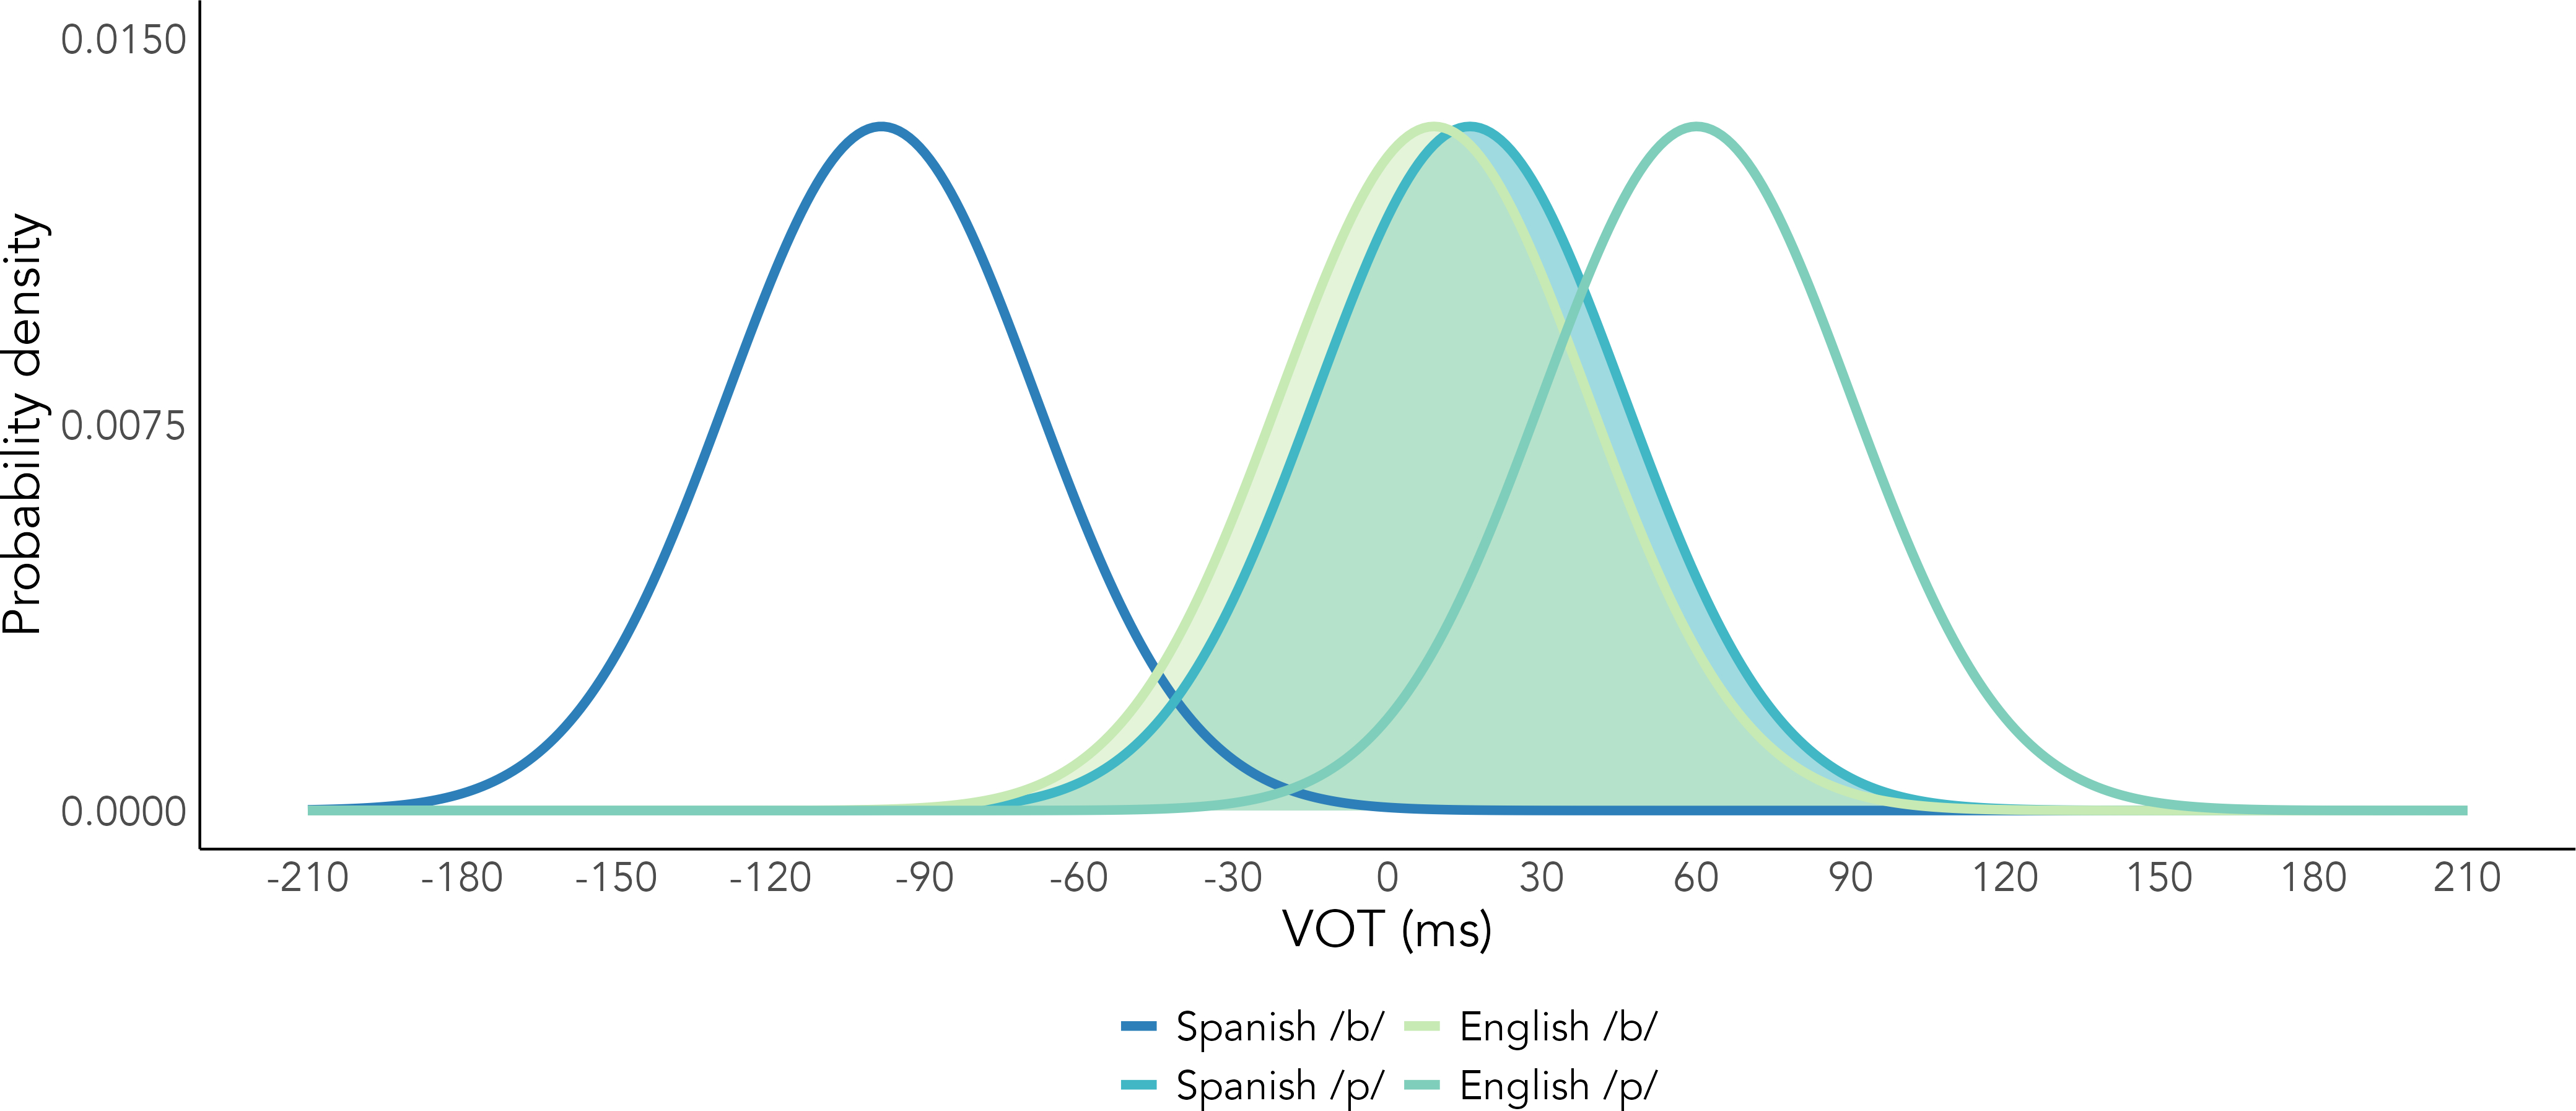
\includegraphics[width=\textwidth]{../14_final_diss/sections/code/outputs/l1_plot} 

}

\caption{Overlapping VOT distributions for Spanish voiceless stops and English voiced stops.}\label{fig:intro-fig}
\end{figure}

To return to the notion of two-category assimilation, consider an L1 Spanish speaker who is learning English as an L2.
She already has an established /p/-/b/ contrast in her L1 Spanish that is associated with VOT.
The /p/-/b/ contrast in her L2 English is associated with the same cue in the same direction, such that VOTs for /p/ are longer than those for /b/.
As a result, the English /p/-/b/ contrast will be relatively easy to integrate into her existing phonological system compared to, for example, certain vowel contrasts in English \citep{baigorri2019}.
The same will be true for both the /t/-/d/ and /k/-/g/ contrasts.
However, assimilating the L2 English /p/ to the L1 Spanish /p/ means that the English phoneme will be produced like the Spanish phoneme.
That is, L2 English /p/ will be produced with a short lag VOT (similar to Spanish /p/).
This will create a perceptual problem from a listener's perspective, since short lag VOTs are associated with English /b/, not /p/; without supporting contextual information, listeners may confuse Spanish-accented English /p/ with /b/ (e.g., \emph{park} perceived as \emph{bark}).
To summarize, cross-language transfer in Spanish-accented English can create ambiguity between voiced and voiceless stops \citep{flege1987}.
Thankfully, listeners are adept at resolving such ambiguities through perceptual adaptation.

\hypertarget{adaptation-to-l2-accented-speech}{%
\subsection{Adaptation to L2-accented speech}\label{adaptation-to-l2-accented-speech}}

A formal way of understanding perceptual adaptation is provided by the ideal adapter framework \citep{kleinschmidt2015, kleinschmidt2019}.
This model is built on three core assumptions: (1) the relations between acoustic cues and phonetic categories are probabilistic; (2) novel cue-category relations are incorporated into the perceptual system through statistical learning; and (3) cue distributions covary with socio-indexical categories.
If a listener is an ``ideal adapter,'' then she will be sensitive to the probability distributions of cue-category mappings (1).
Figure \ref{fig:intro-fig} provides examples of the probability distributions for the acoustic cue VOT over the phonetic categories /p/ and /b/.
An ideal adapter is able to form new representations of cue-category distributions or update her existing ones through statistical learning (2).
The specificity of these cue-category representations, called generative models, depends on two factors: how much information is gained about a cue distribution and how well a category predicts a cue by using a particular grouping \citep{kleinschmidt2019}.
An ideal adapter will structure her generative models according to the most ``informative'' and ``useful'' socio-indexical groupings (3).
We will return to the structure of a listener's generative models in relation to L2-accented talkers in Section \ref{intro-gen} after reviewing the relevant literature.

Previous research shows that listeners adapt quickly to L2-accented speech \citep{bent2021}.
A typical experimental design features an exposure phase, in which participants gain experience with a speech pattern, followed by a test phase.
Talker-specific adaptation is the result of hearing the same talker during exposure and test.
For example, participants who train on Talker A during exposure tend to perform better on Talker A during test than participants who train on Talker B \citetext{\citealp{bradlow2008}; \citealp{clarke2004}; \citealp{xie2021}; \citealp{xie2017structure}; \citealp{xie2018}; \citealp[cf.][]{bradlow2023}}.
Talker-independent adaptation, or generalization, is the result of exposure to a type of talker rather than exposure to a specific talker.
For example, participants who train on Talkers A, B, and C with Accent X tend to perform better on Talker D with Accent X than participants who trained on Talkers E, F, and G with Accent Y \citep{alexander2019, bradlow2008, sidaras2009, tzeng2016, xie2021, xie2018}.
Overall, experience with L2-accented talkers improves perception of novel L2-accented talkers \citep{witteman2013, tzeng2024, reinisch2014, bieber2022, baese2013}.

\hypertarget{talker-independent-adaptation-to-l2-accented-speech}{%
\subsubsection{Talker-independent adaptation to L2-accented speech}\label{talker-independent-adaptation-to-l2-accented-speech}}

The pattern of results for talker-independent adaptation becomes more complicated when considering different types of exposure to an accent.
Studies often compare single-talker exposure, in which one talker produces all of the stimuli for a condition, to multi-talker exposure, in which several different talkers produce the stimuli for a condition.
For example, participants in a single-talker exposure condition listen to Talker A with Accent X and participants in a multi-talker exposure condition listen to Talkers B, C, and D with Accent X.
During test, both groups listen to Talker E with Accent X.
Differences in task performance with Talker E index generalization from exposure \citep{baese2013, bradlow2008, xie2017similarity, xie2021}.

Experiment 2 of \citet{bradlow2008} illustrates how exposure generalizes across L2-accented talkers with the same L1.
In this experiment, participants completed a sentence transcription task during both exposure and test, and performance was measured in terms of sentence recognition accuracy.
There were four exposure conditions: talker-specific, multi-talker, single-talker, and control.
Participants in the talker-specific condition trained directly on the Mandarin-accented English test talker, while those in the multi-talker condition were exposed to five novel Mandarin-accented English talkers.
Participants in the single-talker condition were exposed to just one of the Mandarin-accented English talkers from the multi-talker condition.
Control training featured five L1-accented English talkers.
Training was followed by two post-tests: one featured a novel talker with a familiar L2 accent (Mandarin) and the other featured a novel talker with an unfamiliar L2 accent (Slovakian).
Performance on the Mandarin-accented English test talker was higher in the talker-specific and multi-talker conditions than in the single-talker and control conditions, which did not differ from one another.
By contrast, performance on the Slovakian-accented English test talker did not differ between conditions.
These results suggest that exposure to multiple talkers with the same L1 highlights the features that characterize a specific L2 accent.

\citet{baese2013} provided evidence that exposure to multiple L2-accented talkers with \emph{different} L1s also facilitates generalization.
They used the same stimulus materials and procedures as Experiment 2 in \citet{bradlow2008} in order to compare a multi-accent exposure group directly to the multi-talker exposure and control groups from the previous study.
During multi-accent training, participants were exposed to five L2-accented English talkers, each of whom had a different L1: Thai, Korean, Hindi, Romanian, and Mandarin.
Multi-accent and multi-talker exposure yielded higher performance on the Mandarin-accented test talker than control exposure.
Multi-accent exposure also generalized to the Slovakian-accented test talker, while multi-talker and control exposure did not.
Taken together with the results of \citet{bradlow2008}, these results suggest that exposure to multiple L2-accented talkers facilitates talker-independent adaptation to a greater extent than exposure to a single L2-accented talker.
A multi-talker versus single-talker advantage was found even when the L2-accented talkers in the multi-talker condition did not share an L1 with the test talker.
By contrast, \citet{xie2021} and \citet{xie2017similarity} both observed comparable talker-independent adaptation effects for multi- and single-talker conditions.

Specifically, \citet{xie2021} sought to replicate \citet{bradlow2008} with one key change: counterbalancing the test and exposure talkers.
In the original study, different (partially overlapping) sets of Mandarin-accented English talkers were used in the multi-talker and single-talker exposure conditions.
Thus, the lack of generalization from single-talker training may have been the result of the specific talkers, rather than the superiority of multi-talker exposure per se.
The specific combination of exposure and test talkers is likely to have affected performance under both exemplar-based \citep[e.g.,][]{goldinger1998, johnson2006}, and hybrid \citep[e.g.,][]{pierrehumbert2016, kleinschmidt2015} models of speech perception \citep[see Introduction to][]{xie2021}.
To address this potential confound, \citet{xie2021} used a single set of Mandarin-accented talkers for both multi-talker and single-talker exposure; in addition, these talkers were rotated through the exposure talker and test talker roles.
The results replicated \citet{bradlow2008}'s finding that multi-talker exposure facilitates generalization more than control exposure.
However, contrary to \citet{bradlow2008}, they found that single-talker exposure also facilitated generalization more than control exposure.
When comparing multi- and single-talker exposure, the difference in performance depended on the particular combination of exposure and test talkers.
Overall, these results suggest that generalization is strongly influenced by talker-specific features.

\citet{xie2017similarity} investigated the acoustic-phonetic features of the exposure talkers that facilitate generalization.
In this study, participants were exposed to Mandarin-accented English through an auditory lexical decision task.
Experimental exposure included multisyllabic real words that biased listeners toward perceiving ambiguous word-final stops as /d/ rather than as /t/ (e.g., \emph{overload}).
Control exposure did not include these critical items.
Both types of exposure featured five Mandarin-accented talkers; the only difference was in the presence of disambiguating lexical contexts for learning ambiguous word-final /d/.
During test, participants performed a primed cross-modal lexical decision task with a novel Mandarin-accented talker.
Previous exposure to Mandarin-accented word-final English /d/ in disambiguating lexical contexts generalized to the novel talker.
Specifically, lexical activation for the /d/-final member of minimal pairs like \emph{seed} versus \emph{seat} was increased in the experimental versus the control group.
The results suggest that listeners did not simply expand their phonetic category boundaries with exposure; instead, they used the lexical contexts from training to re-tune their categories for particular accented features.

Two follow-up experiments with single-talker exposure revealed the importance of exposure-test similarity.
Of the five talkers included in the multi-talker exposure, two were selected.
The first talker was the dissimilar talker, who differed from the test talker on the three key acoustic measures associated with the word-final /t/-/d/ contrast.
The second talker was the similar talker, who did not differ from the test talker in the means of these measures.
Exposure to the similar talker generalized to the test talker, with experimental exposure decreasing lexical competition between \emph{seed}-\emph{seat} minimal pairs compared to control exposure.
By contrast, exposure to the dissimilar talker did not increase performance relative to control exposure.
Moreover, generalization from the similar talker was as strong as generalization from multi-talker exposure (which included the similar talker).
Together, the results of \citet{xie2017similarity} show that the correspondence between exposure and test talkers at the acoustic-phonetic level is critical for understanding the observed patterns of generalization across studies.

\hypertarget{competing-hypotheses-for-generalization}{%
\subsubsection{Competing hypotheses for generalization}\label{competing-hypotheses-for-generalization}}

There are two competing explanations for why multi-talker exposure may or may not provide additional benefits for generalization over single-talker exposure: the exposure-to-variability hypothesis and the similarity-based hypothesis.

The exposure-to-variability hypothesis posits that L2-accented talkers exhibit similarities in production that differ from L1-accented norms \citep{baese2013}.
The exposure-to-variability hypothesis also posits that among L2-accented talkers with the \emph{same L1}, cross-language influence shifts the relations between acoustic cues and phonetic categories similarly across talkers.
Among L2-accented talkers with \emph{different L1s}, typological features that are unique to the L2 lead to similarly accented realizations regardless of the L1.
Multi-talker exposure thus allows listeners to abstract away from the peculiarities of any given talker and home in on these commonalities.
For example, a listener encountering one unfamiliar Spanish-accented talker may not know whether their short lag VOTs are specific to that talker or characteristic of the L2 accent.
By contrast, a listener encountering multiple unfamiliar Spanish-accented talkers at once would not only see that short lag VOTs are common across the talkers, but also that other accent features (e.g., vowel height) exhibit covariation with voicing \citep{clayards2017}.
In \citet{bradlow2008}, multi-talker exposure outperformed single-talker exposure, suggesting that training on multiple L2-accented talkers (with the same L1) allowed listeners to separate the characteristic features of an accent from the idiosyncratic features of a talker.
The results of \citet{bradlow2008} support the exposure-to-variability hypothesis, but do not align with the effects observed by \citet{xie2017similarity} and \citet{xie2021}.

By contrast, the similarity-based hypothesis posits that acoustic-phonetic overlap between the exposure and test talkers, rather than variability during exposure, facilitates generalization \citep{xie2021}.
In \citet{xie2017similarity}, listeners exhibited comparable talker-independent adaptation effects after both single- and multi-talker exposure to Mandarin-accented realizations of word-final /d/, which is perceptually confusable with /t/ (e.g., \emph{seed} vs.~\emph{seat}).
Critically, both exposure conditions contained a Mandarin-accented talker with similar word-final /d/ acoustics to the test talker.
\citet{xie2021} also demonstrated equivalent generalization effects from single- and multi-talker exposure to Mandarin-accented speech.
They argue that exposure to multiple talkers merely increases the likelihood that listeners will encounter a cue distribution that is relevant for adapting to the test talker.
For example, multi-talker training on Spanish-accented speech is more likely to include at least one talker with short lag VOTs than single-talker training.
\citet{bradlow2008}'s multi-talker exposure condition may have included talkers who were more similar to the test talker than their single-talker exposure condition, which would confound talker similarity and exposure to variability.
\citet{xie2021} addressed this confound by counterbalancing the combinations of exposure and test talkers across participants.
Thus, the similarity-based hypothesis may account for the differential effects of single- and multi-talker exposure in perceptual adaptation studies.
The present study was designed to distinguish between the roles of variability and similarity in talker-independent adaptation.
To summarize, the similarity-based hypothesis focuses on specific cue-category mappings, while the exposure-to-variability hypothesis focuses on the covariation between cues.

\hypertarget{intro-gen}{%
\subsection{Comparing variability and similarity}\label{intro-gen}}

As discussed above, the results of \citet{bradlow2008} support the exposure-to-variability hypothesis, while those of \citet{xie2017similarity} and \citet{xie2021} support the similarity-based hypothesis.
We argue that the socio-indexical structure of cue-category mappings in the ideal adapter framework provides a link between these two hypotheses and can account for these conflicting findings \citep{kleinschmidt2019}.
According to the ideal adapter framework, listeners represent each cue-category mapping according to informative and useful groupings.
For L2-accented speech, these groupings may be structured according to each talker (talker-specific) or to the L2 accent shared by the talkers (talker-independent).

The exposure-to-variability hypothesis argues that increasing variability during exposure increases systematic covariation among relevant cues, enabling listeners to separate the idiosyncratic features of a talker from the common features of an accent.
To restate this hypothesis in terms of the ideal adapter framework, covariation among individual exposure talkers promotes the development of a robust talker-independent model (or refinement of an existing one).
In turn, this talker-independent model guides adaptation to the novel test talker.
This exposure-to-variability perspective assumes that talker-independent models are better for generalization than talker-specific models.

By contrast, the similarity-based hypothesis argues that increasing the similarity between the cue-category mappings of the exposure and test talkers facilitates generalization.
Translating this hypothesis into the ideal adapter framework, listeners develop robust talker-specific models during exposure.
During test, listeners use the model that provides the most information about the test talker's cue distributions and most readily predicts their individual cue values to guide adaptation.
This similarity-based perspective assumes that talker-specific models are best for generalization because they provide precise information about cue-category mappings.

Overall, the specificity of a listener's set of generative models may explain the effects of variability and similarity on generalization.
The present study tests these two hypotheses in order to probe the mechanisms underlying adaptation to L2-accented speech.
The overarching goal is to understand how the L1 speech recognition system learns the patterns of cross-language influence in L2 speech production.

\hypertarget{present-study}{%
\subsection{Present study}\label{present-study}}

How do listeners generalize their experience with L2-accented speech?
On the one hand, the \emph{structure} of exposure may be the primary driver of talker-independent adaptation.
Variability has been the primary focus of structural inquiries \citep{baese2013}, with the number of talkers being the key manipulation \citep{bradlow2008, bieber2022, choi2019, xie2021}.
On the other hand, the \emph{content} of exposure may be the key to effective generalization.
At a high level, training on the relevant L2 accent tends to facilitate talker-independent adaptation \citep{bradlow2023, clarke2004, xie2018, alexander2019}.
At a detailed level, exposure to the relevant acoustic-phonetic features of an L2 accent explains generalization beyond shared L1 \citep{xie2017similarity, sidaras2009, reinisch2014}.
Together, a shared L1 and common acoustic-phonetic features create similarity between exposure and test talkers that facilitates adaptation.
The present study builds on this body of work investigating generalization of L2-accented speech.
The key difference between our study and earlier work is the operationalization of variability and similarity.
Specifically, we increased the precision with which variability was implemented \citep[c.f.][]{baese2013} and expanded the scope of similarity \citep[c.f.][]{xie2017similarity} in order to better delineate the exposure-to-variability and similarity-based hypotheses.
The goal was to clarify some of the inconsistent findings in the literature for talker-independent adaptation to L2-accented speech \citep{bent2021}.

Regarding variability, previous studies have almost exclusively investigated this factor as a comparison between single-talker exposure and multi-talker exposure \citep[c.f.][]{baese2013, bradlow2023}.
However, multi-talker exposure reduces the amount of experience with any given talker relative to single-talker exposure.
From the larger perceptual adaptation literature, we know that listeners are highly sensitive to acoustic-phonetic mappings and use them to adapt to new talkers \citep[e.g.,][]{kraljic2006}.
We also know that there is a high degree of within- and between-talker variability in both L1- and L2-accented speech production \citep{xie2020, wade2007}.
Depending on the idiosyncrasies of a given exposure talker, altering the amount of experience with this talker may benefit or impede generalization.
This asymmetry in talker-specific exposure may explain some of the inconsistent findings in the literature \citep{xie2017similarity, xie2021}.
Moreover, exposure to multiple talkers increases the sources of covariation to account for, which in turn increases the difficulty of accounting for them during exposure.
If we assume, as the exposure-to-variability hypothesis does, that experience with covariation is critical for generalization, this lack of clarity obscures how and why variability might facilitate generalization.
In the present study, we used a single group of talkers with the same L1 to control the type and amount of experience with each talker across levels of variability.

Regarding similarity, previous studies have either conceptualized this factor at the accent level or at the acoustic-phonetic level.
When it comes to operationalizing either definition of similarity, we run into the same problem as we did with multi-talker versus single-talker exposure.
That is, we end up comparing two (or more) groups of exposure talkers between conditions.
If we assume again that listeners are highly sensitive to talker-specific acoustic-phonetic features, then this design confounds talker- and accent-specific effects.
In other words, we cannot know whether listeners are ``learning a talker or learning an accent'' or learning both \citep{xie2017similarity}.
Here, we manipulated the stimuli listeners encounter during exposure rather than the talkers in order to maintain consistency across levels of similarity.
Moreover, we directly crossed the factors of similarity and variability in the same design, which, to our knowledge, has not yet been done.
Overall, this study allows us to address the ongoing debate between the exposure-to-variability and similarity-based hypotheses for generalization.

\hypertarget{norming-study}{%
\section{Norming study}\label{norming-study}}

\hypertarget{methods-pars-norm}{%
\subsection{Participants}\label{methods-pars-norm}}

Prior to conducting the main experiments, we recruited a separate group of participants (\emph{N} = 688) from the Penn State subject pool to norm the auditory stimuli.
Participants provided implied consent in line with Penn State IRB policies and were compensated 0.5 class credits after completing the experiment, which took 15-30 minutes.
Eligible participants were between the ages of 18 and 40 years, spoke English as their first and only fluent language, had normal hearing, had normal or corrected-to-normal vision, and did not have a history of language-related disorders.
We removed ineligible participants (\emph{N} = 34) and those with poor data quality (\emph{N} = 83; see Section \ref{methods-analysis-norm}) from further analysis.
This left 571 participants.

\hypertarget{methods-stims}{%
\subsection{Stimuli}\label{methods-stims}}

Stimuli were grouped by onset phoneme (e.g., \emph{park} has the onset phoneme /p/).
There were three \textbf{experimental onset} groups: critical, competitor, and control.
Critical onsets were voiceless stops (/p/, /t/, and /k/), competitor onsets were voiced stops (/b/, /d/, and /g/), and control onsets were voiceless fricatives (/f/, /s/, and /\textipa{S}/).
Across the experimental onset groups, phonemes were also grouped (roughly) according to their place of articulation: labial (/p/, /b/, and /f/), alveolar (/t/, /d/, and /s/), and postalveolar/velar (/k/, /g/, and /\textipa{S}/).
These will be referred to as the \textbf{cross-experimental onset} groups.
There was one \textbf{filler onset} group: /m/, /n/, /l/, /\textipa{\*r}/, /h/, and /w/.
Filler onsets were also grouped by their place of articulation: nasal (/m/ or /n/), alveolar (/l/ or /\textipa{\*r}/), and other back consonants (/h/ or /w/).
These will be referred to as the \textbf{within-filler onset} groups.
Finally, each cross-experimental onset group was paired with one of the within-filler onset groups according to frontness/backness: front (/p/, /b/, /f/, /m/, and /n/), mid (/t/, /d/, /s/, /l/, and /\textipa{\*r}/), and back (/k/, /g/, /\textipa{S}/, /h/, and /w/).
These will be referred to as the \textbf{cross-condition onset} groups.

Stimulus selection began by downloading real words with one to four syllables, three to eight letters, and one to two morphemes from the English Lexicon Project (ELP) restricted lexicon \citep{balota2007}.
Within this set of items, we limited our search to words with experimental or filler onsets followed directly by a vowel (e.g., \emph{peach} was considered but \emph{preach} was not).
We removed duplicate word stems with different suffixes (e.g., \emph{paints} and \emph{painting} were removed but \emph{paint} was kept).
We also removed any inappropriate, harmful, or distracting words and word stems.
The remaining set of items will be referred to as the ELP pool.

Multisyllabic stimulus selection began by drawing real words with two to four syllables, five to eight letters, and one to two morphemes from the ELP pool.
We removed words with minimal pairs between the critical and competitor groups (e.g., \emph{pocket} and \emph{docket} were removed but \emph{socket} and \emph{locket} were kept).
Once the set of options was established, real words were selected and pseudowords were created.
Pseudowords were created by changing the onsets of real words with filler onsets that had not been selected as potential real words for the study.
For experimental pseudowords, onsets were assigned according to the cross-condition onset groups (e.g., \emph{machine} became *\emph{pachine}, *\emph{bachine}, and *\emph{fachine}).
For filler pseudowords, one of the other five filler onsets was substituted for the existing filler onset (e.g., \emph{medicine} became *\emph{hedicine}).
In total, 544 multisyllabic real words and 555 multisyllabic pseudowords were normed.

Monosyllabic stimulus selection began by drawing real words with one syllable, three to six letters, and one morpheme from the ELP pool.
From this set of options, we pulled all words with critical onsets that had cross-experimental minimal pairs with competitor onsets (e.g., \emph{park}-\emph{bark}).
Both members of each critical-competitor minimal pair were normed.
We also selected words with filler onsets that had a minimal pair with a different filler onset (e.g., \emph{mall}-\emph{hall}).
In total, 319 monosyllabic real words were normed.

Norming took place in three waves of testing.
Overall, there were nine experimental lists of 180 to 540 items: three in the first wave, two in the second, and four in the third.
Lists always contained an equal number of real words and pseudowords, and items from each experimental onset groups were always presented in separate lists.

\hypertarget{methods-rec}{%
\subsection{Recording}\label{methods-rec}}

One female L1-accented English talker from the US (Talker 0; the first author) recorded all items.
Audio was captured with a head-worn condenser microphone (Shure SM35-XLR) connected to an audio interface (Sound Devices USBPre2) and recorded with Praat \citep{broersma2021} in mono at 44.1 kHz in a sound-attenuated booth.
After annotating the recordings and extracting the individual sound files, stimuli were normalized to 70 dB and had 50 ms of silence added to the beginning and end.

\hypertarget{task-and-procedure}{%
\subsection{Task and procedure}\label{task-and-procedure}}

The study was conducted online using Pavlovia.
At the beginning of the study, participants responded to a yes/no question for each eligibility criterion.
Ineligible participants were not able to complete the study.

The study featured an auditory lexical decision task.
Participants were randomly assigned to an experimental list.
On each trial, participants indicated whether an auditory stimulus was a real English word or not by pressing the \emph{d} or \emph{k} key on their keyboard.
One of the two response-key relations---real-\emph{d} or real-\emph{k}---was assigned randomly to each participant.
The total number of trials varied by list.

\hypertarget{methods-analysis-norm}{%
\subsection{Analysis}\label{methods-analysis-norm}}

Analyses were conducted with R version 4.2.2 using the \emph{stats} package \citep{rcore2022}.
Each wave of testing was analyzed separately.
The experimental lists within each wave were combined for analysis.
We first conducted one-sample t-tests comparing each participant's accuracy to chance (50\%) to check for data quality.
Data from participants whose performance was indistinguishable from chance were removed from further analysis (see Section \ref{methods-pars-norm}).
Next, we conducted one-sample t-tests comparing the accuracy on each item to chance (50\%).
Items that did not yield above-chance accuracy were removed from further consideration.
All three variants of each experimental pseudoword and both members of each cross-experimental minimal pair needed to have above-chance accuracy in order to be considered for final selection.
The set of items that passed the norming phase will be referred to as the selection pool.
For details on the stimuli that were selected for Experiment 1, see Section \ref{methods-lists-1a}.

\hypertarget{experiment-1-investigating-differences-in-generalization-from-exposure-to-spanish-accented-stops-versus-fricatives}{%
\section{Experiment 1: Investigating differences in generalization from exposure to Spanish-accented stops versus fricatives}\label{experiment-1-investigating-differences-in-generalization-from-exposure-to-spanish-accented-stops-versus-fricatives}}

XX It would be good to briefly describe the main research question and theory-guided predictions.

\hypertarget{methods}{%
\subsection{Methods}\label{methods}}

We used an exposure-test design to understand how different kinds of experience with Spanish-accented speech change listeners' VOT-stop mappings.
The exposure phase established the comparison between the similarity-based and exposure-to-variability hypotheses of talker-independent adaptation.
The test phase assessed the effects of each type of exposure on perception.

\hypertarget{methods-design-1a}{%
\subsubsection{Design}\label{methods-design-1a}}

Participants were exposed to multisyllabic real words and pseudowords before being tested on monosyllabic real words.
Participants heard these items produced by four Spanish-accented talkers: three during exposure and one during test.
During exposure, multisyllabic items without onset competitors provided disambiguating lexical contexts for categorizing Spanish-accented onsets.
For example, consider the real word \emph{pencil} and the pseudoword *\emph{pachine}.
In both cases, the onset may be interpreted as /p/ or /b/.
This ambiguity does not affect whether *\emph{pachine} is perceived as a real word or not, since both *\emph{pachine} and *\emph{bachine} are pseudowords.
However, resolving this ambiguity is necessary for distinguishing between the real word \emph{pencil} and pseudoword *\emph{bencil}.
Critically, participants hearing ambiguous real words like \emph{pencil} would never hear unambiguous real words like \emph{beehive}.
Thus, in the context of the exposure task, participants should learn to perceive the ambiguous short lag VOTs as /p/ rather than as /b/.
During test, monosyllabic items with onset competitors created ambiguous lexical contexts in which to assess learning from exposure.

\textbf{Exposure similarity} was operationalized as the relation between the experimental onsets encountered during exposure and the critical onsets encountered during test.
There were three levels of Similarity: Direct, Indirect, and Control.
Each level refers to the type of information participants received about Spanish-accented voiceless stops.
In Direct conditions, participants were exposed directly to critical onsets (e.g., \emph{peanut} and *\emph{pachine}).
In Indirect conditions, participants were exposed to competitor onsets (e.g., \emph{beehive} and *\emph{bachine}), thereby gaining experience with the shifted VOT continuum that they would encounter during test.
In Control conditions, participants were exposed to control onsets (e.g., \emph{football} and *\emph{fachine}), thereby gaining general experience with Spanish-accented speech but not with stop VOTs.
This design allowed the talkers to remain the same across the three levels of Similarity.

\textbf{Exposure variability} was operationalized as the relation between onset phonemes and exposure talkers.
There were two levels of Variability: Invariant and Variant.
Each level refers to the type of experience with each talker.
This is illustrated in Figure \ref{fig:exp1-fig}.
In Invariant conditions, listeners heard each of the three exposure talkers produce one onset out of the three in an experimental group (e.g., Direct-Invariant: Talker A produced \emph{peanut}, \emph{palace}, and \emph{pianist}; Talker B produced \emph{terminal}, \emph{tiara}, and \emph{textile}; and Talker C produced \emph{kingdom}, \emph{counter}, and \emph{kayak}).
This means that all of the words with a given onset were produced by only one talker.
In Variant conditions, listeners heard each of the three exposure talkers produce all three onsets in an experimental group (e.g., Direct-Variant: Talker A produced \emph{peanut}, \emph{terminal}, and \emph{kingdom}; Talker B produced \emph{palace}, \emph{tiara}, and \emph{counter}; and Talker C produced \emph{pianist}, \emph{textile}, and \emph{kayak}).
This means that one third of the words with a given onset were produced by each talker.
This design allowed the items and talkers to remain the same between levels of Variability.

The two exposure factors of Similarity (Direct, Indirect, Unrelated) and Variability (Variant, Invariant) were manipulated between participants, so each participant was assigned to one of the six combinations of Similarity and Variability.
Target type was manipulated within participants.
There were three levels of Target: Identity, Competitor, and Unrelated (See Figure \ref{fig:exp1-fig}).
Each level refers to the type of visual target that followed each auditory prime.
Identity targets exactly matched the auditory primes (e.g., \emph{park}-\emph{park}).
Competitor targets were the minimal pairs of the auditory primes (e.g., \emph{park}-\emph{bark}).
Unrelated targets only shared vowels with the auditory primes (e.g., \emph{park}-\emph{wand}).
Differential performance on these three conditions indexed learning from exposure.

\begin{figure}

{\centering 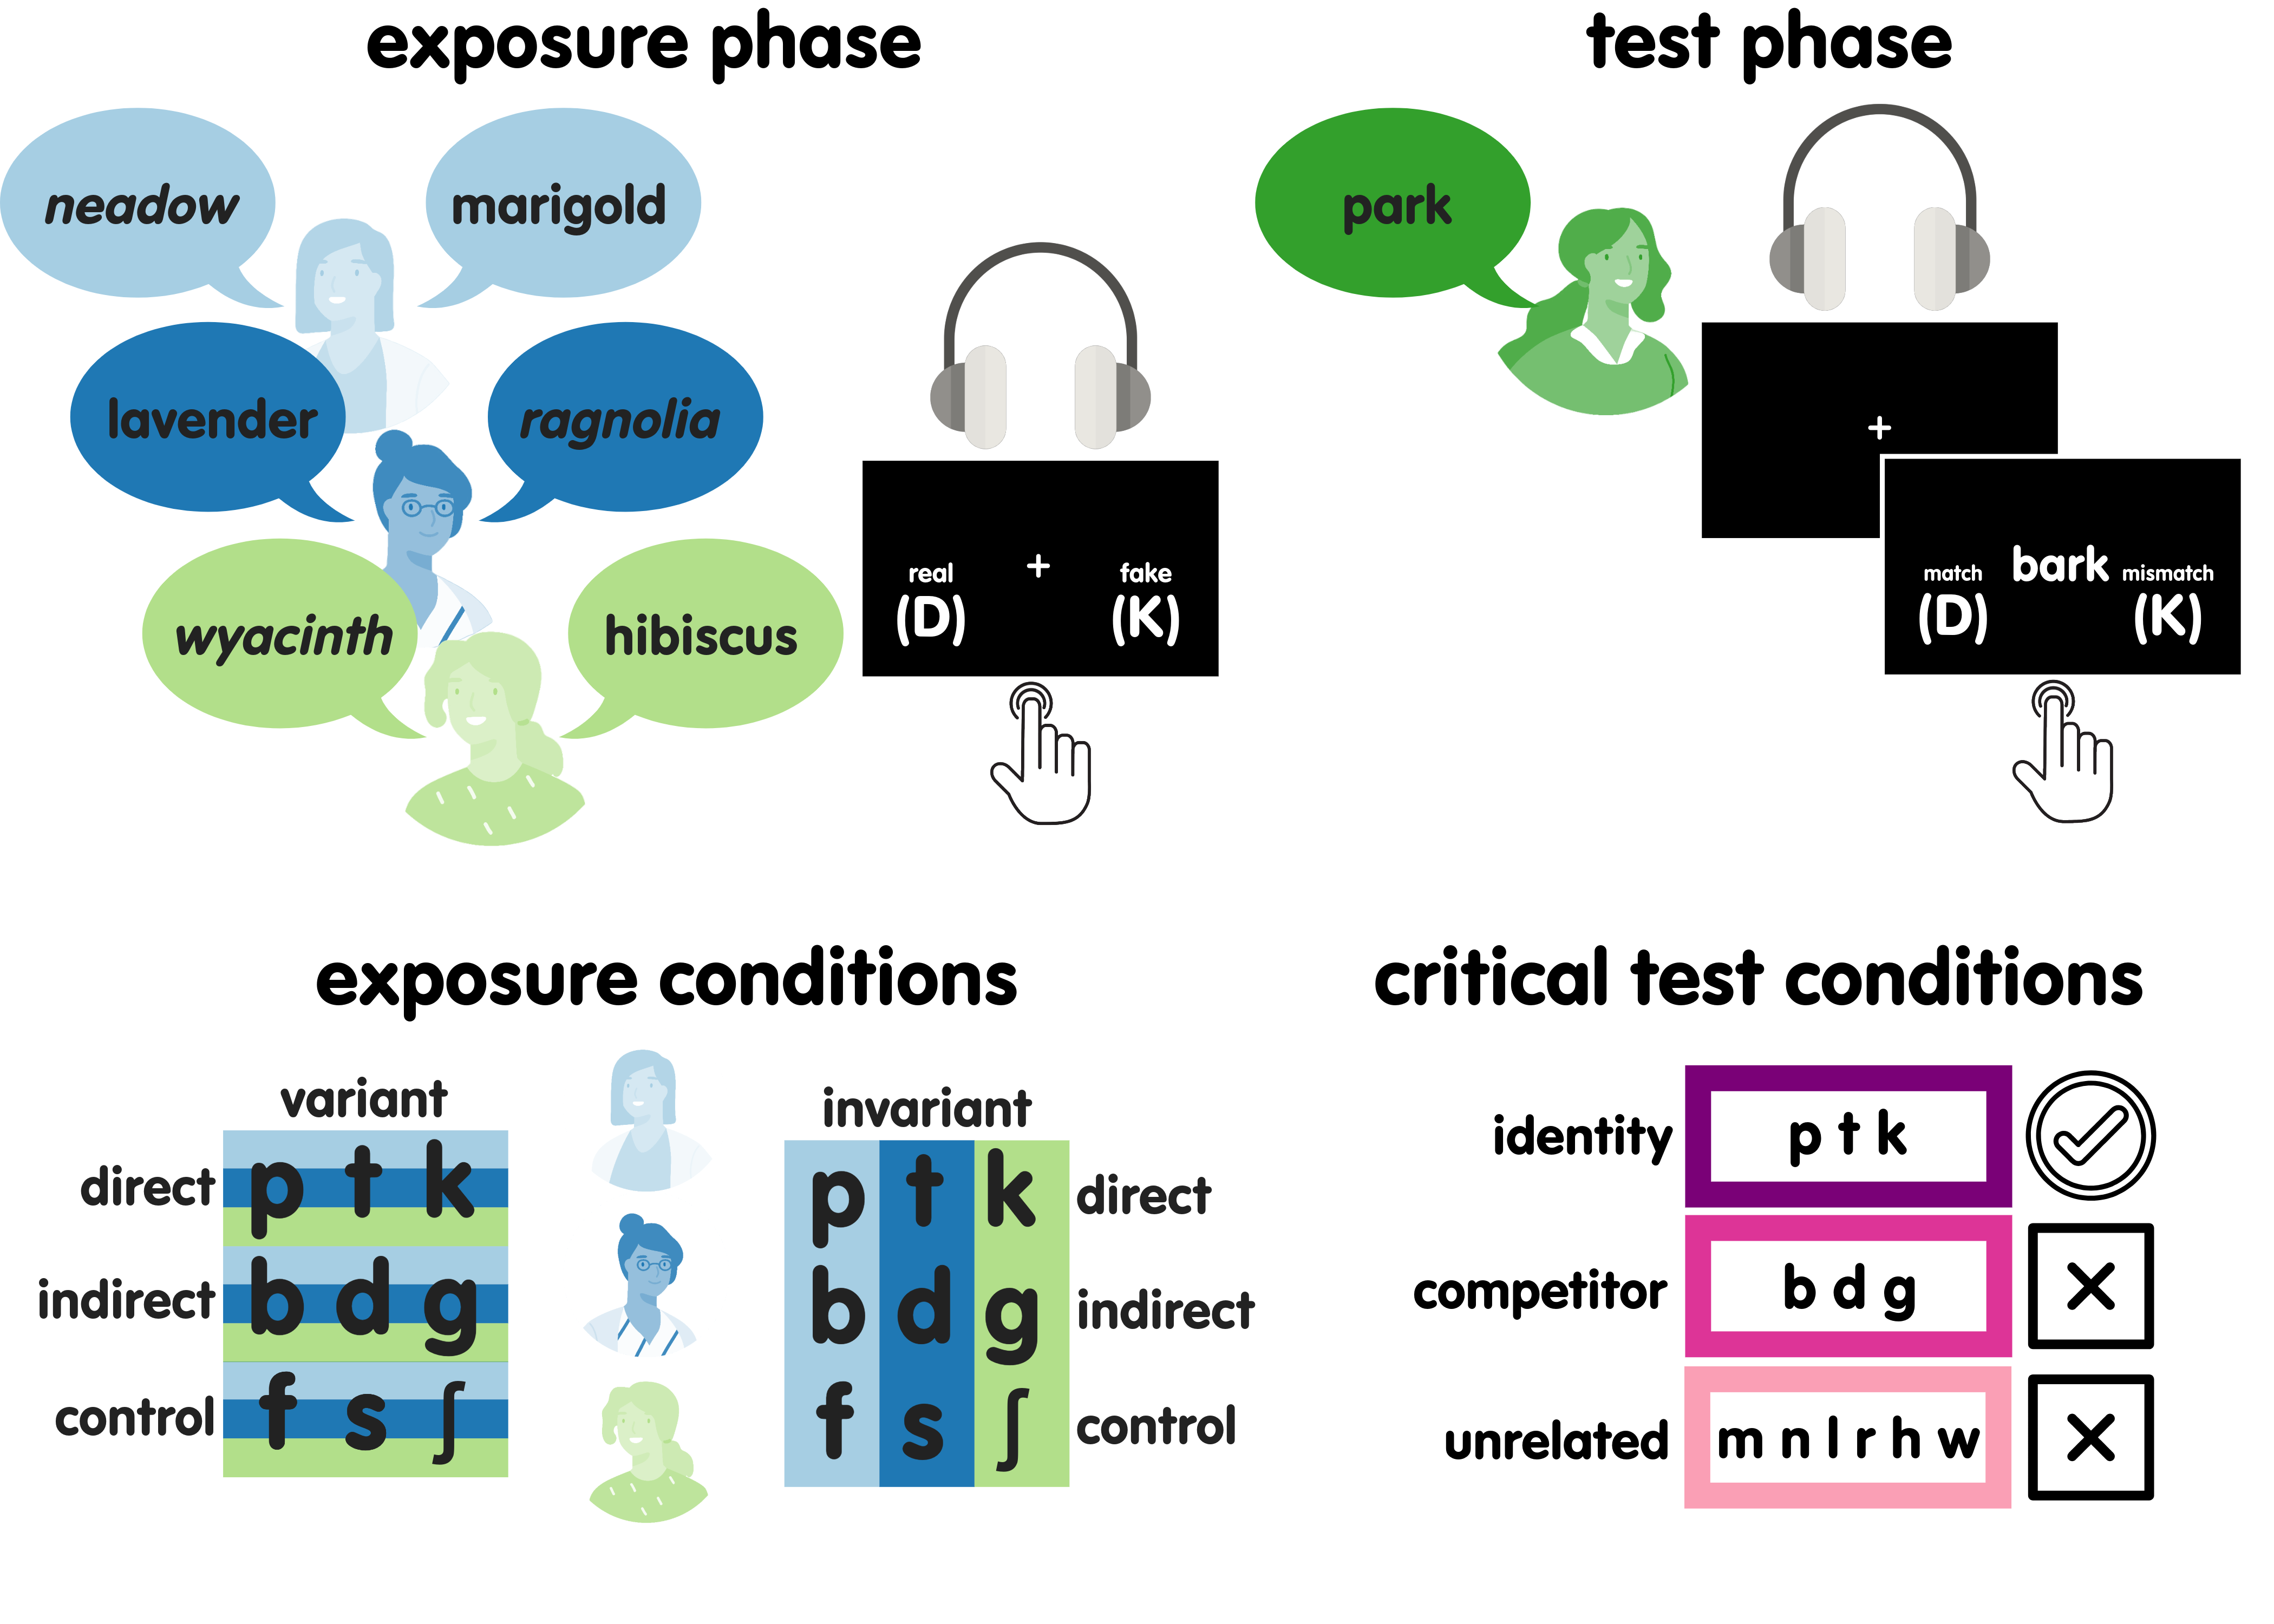
\includegraphics[width=\textwidth]{../14_final_diss/figures/diss_1} 

}

\caption{Experiment 1 design. The exposure phase panel illustrates the task with filler real words and pseudowords.}\label{fig:exp1-fig}
\end{figure}

\hypertarget{methods-pars-1a}{%
\subsubsection{Participants}\label{methods-pars-1a}}

We recruited 296 participants through the online platform Prolific.
Participants provided implied consent in line with Penn State IRB policies and were compensated \$6 after completing the experiment, which took approximately 30 minutes.
The experiment was available to individuals whose Prolific user profiles aligned with the following eligibility criteria: between 18 and 40 years of age, located in the US at the time of the study, English as their first and only fluent language, normal hearing, normal or corrected-to-normal vision, and without a history of language-related disorders.
The Prolific user profiles for each participant also included sex (two options, select one) and race/ethnicity information (four options, select all that apply).

The eligibility criteria were cross-checked with the responses to a post-experiment questionnaire (see Section \ref{methods-tasks-1a}), and any ineligible participants was removed from further analysis (\emph{N} = 9).
We also removed participants with any knowledge of Spanish, with self-rated proficiency greater than or equal to 3/5 in any languages other than English, with self-rated proficiency less than 5/5 in English, or whose place of origin was not the US (\emph{N} = 15).
This left 287 eligible participants.

Finally, we removed participants with poor data quality from further analysis (\emph{N} = 15).
Poor data quality was defined as: accuracy statistically indistinguishable from or significantly below chance on experimental real words in the exposure task, zero correct experimental trials in any of the three conditions in the test task, or fewer than 50\% of experimental trials with correct responses and reaction times between 50 and 2500 ms in either task (see Section \ref{methods-tasks-1a} for details).
This left 257 participants for analysis (Age: \emph{M} = 31, \emph{SD} = 6, Min = 18, Max = 40; Sex: Female = 121, Male = 135, Prefer not to say = 1; Race: Asian = 5, Black = 43, Multiple selected = 21, Other = 5, White = 182, Not provided = 1).

We recruited 46 additional participants through Prolific to complete the experiment without the exposure phase.
Removing ineligible participants left 38 participants.
Removing participants with low data quality left 37 participants for analysis (Age: \emph{M} = 31, \emph{SD} = 5, Min = 21, Max = 40; Sex: Female = 19, Male = 18; Race: Asian = 2, Multiple selected = 5, Other = 2, White = 28).
All aspects of recruitment were the same for this group as for the main group of participants.

\hypertarget{methods-talk-1a}{%
\subsubsection{Talkers}\label{methods-talk-1a}}

Seven female Spanish-accented English talkers from Latin America and Spain were recruited to be talkers for the experiment.
Talkers were compensated with one \$20 Amazon giftcard per recording session (30-60 minutes each; 1-2 total).
Recording followed the procedure described in Section \ref{methods-rec}.

Out of the seven talkers, we selected four from Mexico (Talkers 1-4) to control for country-level dialectal variation in the L1.
Each talker was from a different region of Mexico and reported living in this region for the majority of their lives before moving to the US for college or graduate school.
All four talkers reported that they grew up speaking Spanish with their caregivers and began acquiring English in traditional classroom settings.
Language background information for each talker is provided in Table \ref{tab:spk-tab}.

\begin{table}

\caption{\label{tab:spk-tab}Talker background information.}
\centering
\resizebox{\linewidth}{!}{
\begin{tabular}[t]{r|l|r|r|r}
\hline
Talker & Region & Age of English acquisition & Age of arrival in US & Age at time of recording\\
\hline
1 & Veracruz, Mexico & 10 & 18 & 26\\
\hline
2 & Quintana Roo, Mexico & 13 & 26 & 28\\
\hline
3 & Puebla, Mexico & 5 & 24 & 27\\
\hline
4 & Mexico City, Mexico & 5 & 28 & 31\\
\hline
\end{tabular}}
\end{table}

\hypertarget{methods-stims-1a}{%
\subsubsection{Stimuli}\label{methods-stims-1a}}

In total, there were 936 auditory items and 648 visual items across tasks.
The exposure task featured multisyllabic real words and pseudowords with experimental and filler onsets from the selection pool.
The final set of exposure items included 360 real words (24 per onset) and 360 pseudowords (24 per onset).
The test task featured two types of stimuli: auditory primes and visual targets.
Auditory primes were monosyllabic real words with critical or filler onsets from the selection pool.
The final set of auditory primes included 216 real words (24 per onset).
The final set of visual targets included 648 real words (3 per prime).

During auditory stimulus selection, we considered a number of parameters.
From the ELP, we included word length, orthographic neighborhood density (OND), phonological neighborhood density (PND), and US Zipf frequency.
From \citet{brysbaert2019}, we included percent known and prevalence.
We also included the position of lexical stress, calculated from the pronunciation information provided by the ELP, and mean lexical decision accuracy from norming (LDT).
The final set of exposure real words was chosen such that the four groups of stimuli---Direct, Indirect, Control, and Filler---were matched on each of these parameters.
We conducted two-sample t-tests comparing each group on each parameter to ensure that they were not significantly different (\emph{ps} \textgreater{} .05).
The final set of auditory primes for the test task was selected in a similar way.
We conducted two-sample t-tests comparing the Critical and Filler primes on every parameter except for lexical stress, which was not relevant for monosyllabic words (\emph{ps} \textgreater{} .05).
We also conducted paired t-tests between Critical primes and their Competitor pairs (\emph{ps} \textgreater{} .05).
The final set of exposure pseudowords was chosen such that the four groups of stimuli were matched on length, position of lexical stress, and mean lexical decision accuracy.
The other parameters were either not available (OND and PND) or not relevant (US Zipf frequency, percent known, prevalence) for the pseudowords.
The relevant parameters for each group of stimuli are shown in Table \ref{tab:stim-tab}.
Descriptive statistics for each talker's real word VOTs by onset are provided in Table \ref{tab:spk-vot-tab} (see Section \ref{explore-spk}).

\begin{table}

\caption{\label{tab:stim-tab}Mean and standard deviation of stimulus parameters by condition and task.}
\centering
\resizebox{\linewidth}{!}{
\begin{tabular}[t]{l|l|l|r|l|l|l|l|l|l|l|l}
\hline
Phase & Word type & Condition & N & Length & LDT & Lexical stress & OND & PND & Frequency & Percent known & Prevalence\\
\hline
 &  & Direct & 72 & 6.85 (0.93) & 0.89 (0.09) & 1.11 (0.32) & 0.56 (1.40) & 1.12 (2.13) & 3.38 (0.74) & 0.98 (0.02) & 2.12 (0.29)\\
\cline{3-12}
 &  & Indirect & 72 & 6.82 (0.98) & 0.89 (0.08) & 1.21 (0.41) & 0.62 (1.34) & 1.14 (2.04) & 3.45 (0.72) & 0.99 (0.02) & 2.16 (0.29)\\
\cline{3-12}
 &  & Control & 72 & 6.93 (0.95) & 0.87 (0.09) & 1.15 (0.36) & 0.67 (1.17) & 1.76 (2.76) & 3.39 (0.77) & 0.98 (0.03) & 2.11 (0.38)\\
\cline{3-12}
 & \multirow{-4}{*}{\raggedright\arraybackslash Real word} & Filler & 144 & 6.83 (0.95) & 0.87 (0.10) & 1.12 (0.32) & 0.78 (1.52) & 1.49 (2.66) & 3.42 (0.77) & 0.98 (0.03) & 2.14 (0.35)\\
\cline{2-12}
 &  & Direct & 72 & 7.08 (0.87) & 0.89 (0.06) & 1.22 (0.42) &  &  &  &  & \\
\cline{3-12}
 &  & Indirect & 72 & 7.08 (0.87) & 0.88 (0.07) & 1.22 (0.42) &  &  &  &  & \\
\cline{3-12}
 &  & Control & 72 & 7.08 (0.87) & 0.88 (0.06) & 1.22 (0.42) &  &  &  &  & \\
\cline{3-12}
\multirow{-8}{*}{\raggedright\arraybackslash Exposure} & \multirow{-4}{*}{\raggedright\arraybackslash Pseudoword} & Filler & 144 & 6.93 (1.01) & 0.88 (0.05) & 1.14 (0.35) &  &  &  &  & \\
\cline{1-12}
 &  & Critical prime & 72 & 3.88 (0.63) & 0.88 (0.07) &  & 11.36 (5.21) & 21.85 (7.96) & 4.15 (0.94) & 0.99 (0.04) & 2.22 (0.34)\\
\cline{3-12}
 &  & Competitor pair & 72 & 3.90 (0.65) & 0.88 (0.08) &  & 10.39 (5.02) & 21.15 (7.12) & 4.09 (1.11) & 0.98 (0.05) & 2.10 (0.42)\\
\cline{3-12}
\multirow{-3}{*}{\raggedright\arraybackslash Test} & \multirow{-3}{*}{\raggedright\arraybackslash Real word} & Filler prime & 144 & 3.90 (0.58) & 0.90 (0.08) &  & 10.49 (4.70) & 22.27 (8.89) & 4.15 (0.97) & 0.99 (0.02) & 2.22 (0.32)\\
\hline
\multicolumn{12}{l}{\rule{0pt}{1em}Competitor pairs were presented as visual targets only}\\
\end{tabular}}
\end{table}

An additional set of six real words and six pseudowords with filler onsets (one per onset per word type) was selected for practice.
Six additional primes with filler onsets (one per onset) were also selected for practice.

Visual targets in the test task were monosyllabic real words with critical, competitor, or filler onsets.
Each auditory prime had three visual targets: one was the prime itself, one was its minimal pair, and one was unrelated.
The first two were determined by the prime, but the third needed to be selected separately.
Each unrelated target had a filler onset and was chosen to have the same vowel as the prime but a different onset and offset.
These items were primarily from the selection pool, but some were from the larger ELP pool.
Two additional unrelated targets were also selected for practice.

\hypertarget{methods-lists-1a}{%
\subsubsection{Experimental lists}\label{methods-lists-1a}}

Combining Similarity and Variability created six between-subjects conditions: Direct-Variant, Direct-Invariant, Indirect-Variant, Indirect-Invariant, Control-Variant, and Control-Invariant.
In addition, one group of participants did not receive any exposure prior to test; this will be referred to as the Test-only condition.
The 288 filler items were the same across conditions and evenly divided by word type---real word and pseudoword---as well as by onset---/m/, /n/, /l/, /\textipa{\*r}/, /h/, and /w/.
The 144 experimental items were evenly divided by onset and word type, with onset differing by level of Similarity: Direct (critical: /p/, /t/, and /k/), Indirect (competitor: /b/, d/, and /g/), and Control (control: /f/, /s/, and /\textipa{S}/).
As a result, there were 24 items per onset per word type.

The assignment of talkers to items differed by level of Variability.
In Invariant conditions, talkers were assigned by cross-condition onset group: front (/p/, /b/, /f/, /m/, and /n/), mid (/t/, /d/, /s/, /l/, and /\textipa{\*r}/), and back/other (/k/, /g/, /\textipa{S}/, /h/, and /w/).
In other words, one talker was assigned to front onsets, one to mid, and one to back/other.
Within a given level of Similarity, this means that each talker produced items with one out of the three experimental onsets and two out of the six filler onsets.
For Variant conditions, one third of each of the items of a given onset and word type (8) was randomly assigned to one of three sets: set 1, set 2, or set 3.
Each set was assigned to one talker.

To counterbalance which talkers were assigned to which items across participants, each Variant item set was paired with one Invariant onset group to create three assignment groups: group 1 (front with set 1), group 2 (mid with set 2), and group 3 (back/other with set 3).
In addition, we also counterbalanced the talkers between the exposure and test phases.
To do this, we added group 4 (test) and rotated the four talkers across these four assignment groups in a Latin square design.
Overall, this resulted in 24 experimental lists for the exposure phase, one for each combination of exposure condition (6) and talker assignment (4).

Regardless of exposure condition, all participants heard the same 216 auditory primes during test.
One third (72) were critical items divided evenly by onset---/p/, /t/, and /k/---and two thirds (144) were filler items divided evenly by onset---/m/, /n/, /l/, /\textipa{\*r}/, /h/, and /w/.
Each onset was divided evenly by target type---Identity, Competitor, and Unrelated.
This resulted in eight items per onset per target type
Three experimental lists were created to counterbalance the combinations of auditory prime and visual target across participants.
Since the test talker was also counterbalanced across participants, this resulted in 12 experimental lists for the test phase, one for each combination of prime-target pair (3) and talker assignment (4).

Exposure practice was presented in Talker 0's voice for all participants.
Test practice was presented according to the participant's talker assignment and Variability condition.
Participants in the Test-only condition completed the test practice in Talker 0's voice.

\hypertarget{methods-tasks-1a}{%
\subsubsection{Tasks}\label{methods-tasks-1a}}

The experiment included a headphone check, exposure task, test task, and post-experiment questionnaire.
All aspects of the experiment were conducted online using Pavlovia.
The headphone check, exposure task, and test task were created in PsychoPy Builder \citep{peirce2019}.
The post-experiment questionnaire was built using Pavlovia's survey platform.

The headphone check followed the anti-phase tone test procedure from \citet{woods2017}.
On each trial, participants listened to three pure tones, one of which was out of phase with the other two.
Participants indicated which of the three tones was the quietest by selecting the appropriate button on the screen: tone 1, tone 2, or tone 3.
There were two trials per response for a total of six trials, which were presented in random order.
Participants using well-functioning headphones should have easily perceived the anti-phase tone as the quietest, while those using loudspeakers should not.
Participants completed the task at most two times.

The exposure phase featured the auditory lexical decision task from \citet{xie2017similarity}.
On each trial, participants indicated whether an auditory stimulus was a real English word or not by pressing the \emph{d} or \emph{k} key on their keyboard.
One of the two response-key relations---real-\emph{d} or real-\emph{k}---was assigned randomly to each participant.
Participants completed 12 practice trials followed by 432 main trials presented in random order.
Half of the practice trials (6) and half of the main trials (216) required real word responses.

The test phase featured a cross-modal matching task adapted from the primed cross-modal lexical decision task in \citet{xie2017similarity}.
On each trial, participants first heard a real word (auditory prime) and then saw a real word written on the screen (visual target).
They indicated whether the visual target matched the auditory prime or not by pressing the \emph{d} or \emph{k} key on their keyboard.
The assignment of responses to keys was carried over from the exposure phase, with \emph{match} responses mapped to the same key as \emph{real word} responses in the exposure task.
Participants completed six practice trials followed by 216 main trials presented in random order.
Half of the practice trials (3) and one third of the main trials (72) required match responses.

The post-experiment questionnaire included two sets of items.
The first set of items related to the talker from the test task.
The second set of items included questions about the participant's own language background and demographics.
This second set of items was used to confirm the participant's eligibility as described in Section \ref{methods-pars-1a}.
All post-experiment questionnaire items are described in detail in the supplementary materials.

\hypertarget{methods-proc}{%
\subsubsection{Procedure}\label{methods-proc}}

Eligible participants accessed the experiment through Prolific.
Once a participant began the experiment, they were randomly assigned to one of the experimental lists.
First, they performed the headphone check.
If the participant achieved fewer than five correct trials out of six, they completed the task again.
Participants who failed the headphone check a second time were not allowed to continue; instead, they were redirected to Prolific and asked to return their submission.
After passing the headphone check, participants continued to the exposure task and completed the practice (participants in the Test-only condition continued straight to the test task).
If a participant scored 50\% or lower on the exposure practice, they were not allowed to continue; instead, they were redirected to Prolific and asked to return their submission.
After successfully completing the practice session, the participant performed the exposure task.
Next, the participant continued to the test task and completed the practice.
Regardless of their performance on the practice, the participant performed the test task.
Immediately following the test task, participants continued to the post-experiment questionnaire.
Once the questionnaire was complete, the participant was redirected to Prolific and received compensation.

\hypertarget{methods-analysis-1a}{%
\subsubsection{Analysis approach}\label{methods-analysis-1a}}

Data processing and analysis were conducted with R version 4.2.2 \citep{rcore2022}.
Filler items were not included in any of the analyses.

Prior to analyzing the exposure task data, we removed responses with RTs less than 50 ms (\emph{N} = 31; 0.03\%).
RT was calculated from the onset of the word.
For the RT analyses, we filtered for correct responses.
We used the \emph{robustbase} package to calculate adjusted boxplot statistics for skewed distributions (such as reaction time), which were used to detect responses with reaction times outside the upper and lower fences \citep{hubert2008}.
These outlier responses were removed from further analysis (\emph{N} = 4630; 4.17\%).
RTs were then inverse-transformed (-1000/RT) for analysis.

Prior to analyzing the test task data, we removed responses with RTs less than 50 ms (\emph{N} = 4; 0.02\%).
RT was calculated from the presentation of the visual target.
RT analyses were restricted to correct responses.
We detected and removed outliers by target type according to the adjusted boxplot statistics (\emph{N} = 898; 4.24\%).
Inverse RTs were used for modeling as in the exposure task analyses.

Mixed-effects models were fitted to trial-level data with the \emph{lme4} package \citep{bates2015}.
Generalized linear mixed-effects models with a binomial family function were used to analyze binary accuracy (1,0).
Linear mixed-effects models were used to analyze inverse RT.
Model fitting began with the full random effects structure that was relevant to the task (see below).
In the case of non-convergence, singularity, or correlations above 0.95, random slopes were successively removed, such that the final model for each analysis reflected the maximally-supported structure \citep{barr2013}.
Type-III analysis-of-deviance tables were calculated and Wald chi-square tests conducted with the \emph{car} package \citep{fox2019}.
Estimated marginal means were calculated and pairwise comparisons conducted with the \emph{emmeans} package \citep{lenth2022}.
Pairwise \emph{p}-values were adjusted with the Hommel method to control the family-wise error rate \citep{blakesley2009}.

Exposure task analyses modeled the effects of Variability, Similarity, Word type, and their interactions on accuracy and RT.
The two levels of Variability and Word type were sum contrast-coded.
The three levels of Similarity were Helmert contrast-coded.
Scaled VOT, trial, and word frequency were included as covariates.
Item and participant were included as random intercepts.
By-participant random slopes were included for Variability, Similarity, and their interaction.

For the test task, we conducted two separate sets of analyses.
The first set of analyses modeled the effects of Exposure, Target, and their interaction on accuracy and RT.
Exposure had seven levels: one for each of the six exposure conditions and one for the Test-only condition.
This factor was simple contrast-coded such that the Test-only condition was the reference level.
The three levels of Target were Helmert contrast-coded.
Scaled VOT, scaled trial, and the interaction between scaled prime frequency and scaled target frequency were included as covariates.
Participant and the interaction between auditory prime and visual target were included as random intercepts.

The second set of analyses modeled the effects of Variability, Similarity, Target, and their interactions on accuracy and RT.
The coding scheme for each variable was the same as in the first test analysis.
The continuous predictors and random intercepts were also the same.
By-participant random slopes were included for Variability, Similarity, and their interaction.

If the first set of analyses did not reveal differences between the exposure and Test-only conditions, the second set of analyses was not conducted.
Only significant effects involving the exposure conditions will be discussed.
All results are available on GitHub (XX).

\hypertarget{predictions}{%
\subsubsection{Predictions}\label{predictions}}

The exposure-to-variability and similarity-based hypotheses make different predictions about the effects of each type of exposure on test.
The similarity-based hypothesis predicts a main effect of Similarity, with test performance increasing from Control to Indirect to Direct exposure.
This prediction follows directly from the ideal adapter framework, such that both talker-specific and talker-independent generative models of VOT-stop distributions can generalize to a test talker; what matters is how similar the exposure model is to the test distribution.

By contrast, the exposure-to-variability hypothesis predicts a main effect of Variability, with better test performance after Variant exposure than after Invariant exposure.
Under this hypothesis, exposure to covariation between cues and categories encourages the formation of talker-independent generative models.
This implies that such models have more utility for categorizing critical onsets than any talker-specific models \citep{kleinschmidt2019}.
The exposure-to-variability hypothesis does not predict effects of Similarity on test performance.

\hypertarget{results}{%
\subsection{Results}\label{results}}

\hypertarget{exposure}{%
\subsubsection{Exposure}\label{exposure}}

For accuracy, there was a significant three-way interaction between Variability, Similarity, and Word type (\(\chi^2\)(2, \emph{N} = 3) = 15.90, \emph{p} \textless{} .001), as well as a significant two-way interaction between Variability and Word type (\(\chi^2\)(1, \emph{N} = 2) = 11.39, \emph{p} \textless{} .001).
For RT, we also observed a significant three-way interaction between Variability, Similarity, and Word type (\(\chi^2\)(2, \emph{N} = 3) = 30.46, \emph{p} \textless{} .001).
In addition, the main effect of Similarity was significant (\(\chi^2\)(2, \emph{N} = 3) = 36.93, \emph{p} \textless{} .001).
To follow up on these effects, we conducted two sets of pairwise comparisons: one between levels of Similarity within each combination of Variability and Word type and another between levels of Variability within each combination of Similarity and Word type.

All of the comparisons for accuracy are shown in the left column of Figure \ref{fig:exp1-exp-fig}.
Within Variant exposure, pseudoword accuracy was higher for Control exposure (\emph{M} = 0.93, 95\% CI {[}0.90, 0.95{]}) compared to Indirect exposure (\emph{M} = 0.88, 95\% CI {[}0.84, 0.91{]}; \emph{z} = 2.52, \emph{p} = .035).
Within Control exposure, real word accuracy was higher for Invariant exposure (\emph{M} = 0.86, 95\% CI {[}0.83, 0.89{]}) compared to Variant exposure (\emph{M} = 0.83, 95\% CI {[}0.78, 0.87{]}; \emph{z} = 2.59, \emph{p} = .010).

All of the comparisons for RT are shown in the right column of Figure \ref{fig:exp1-exp-fig}.
Comparing levels of Similarity revealed overall slower RTs for Control exposure.
Within Variant exposure, pseudoword RTs were slower for Control exposure (\emph{M} = 1361, 95\% CI {[}1310, 1417{]}) compared to Direct exposure (\emph{M} = 1242, 95\% CI {[}1195, 1292{]}; \emph{z} = 3.25, \emph{p} = .003).
In addition, real word RTs were slower for Control exposure (\emph{M} = 1254, 95\% CI {[}1211, 1301{]}) compared to both Direct (\emph{M} = 1110, 95\% CI {[}1074, 1148{]}; \emph{z} = 3.44, \emph{p} = .002) and Indirect (\emph{M} = 1135, 95\% CI {[}1097, 1176{]}; \emph{z} = 2.97, \emph{p} = .006) exposure.
Within Invariant exposure, pseudoword RTs were slower for Control exposure (\emph{M} = 1446, 95\% CI {[}1389, 1508{]}) compared to both Direct (\emph{M} = 1267, 95\% CI {[}1220, 1317{]}; \emph{z} = 4.66, \emph{p} \textless{} .001) and Indirect (\emph{M} = 1277, 95\% CI {[}1229, 1329{]}; \emph{z} = 4.29, \emph{p} \textless{} .001) exposure.
Real word RTs were also slower for Control exposure (\emph{M} = 1254, 95\% CI {[}1211, 1301{]}) compared to both Direct (\emph{M} = 1110, 95\% CI {[}1074, 1148{]}; \emph{z} = 4.93, \emph{p} \textless{} .001) and Indirect (\emph{M} = 1135, 95\% CI {[}1097, 1176{]}; \emph{z} = 3.91, \emph{p} \textless{} .001) exposure.
Comparing levels of Variability revealed differences within Control exposure, such that pseudoword RTs were slower for Invariant exposure than for Variant exposure (\emph{z} = 2.33, \emph{p} = .020).

\begin{figure}

{\centering 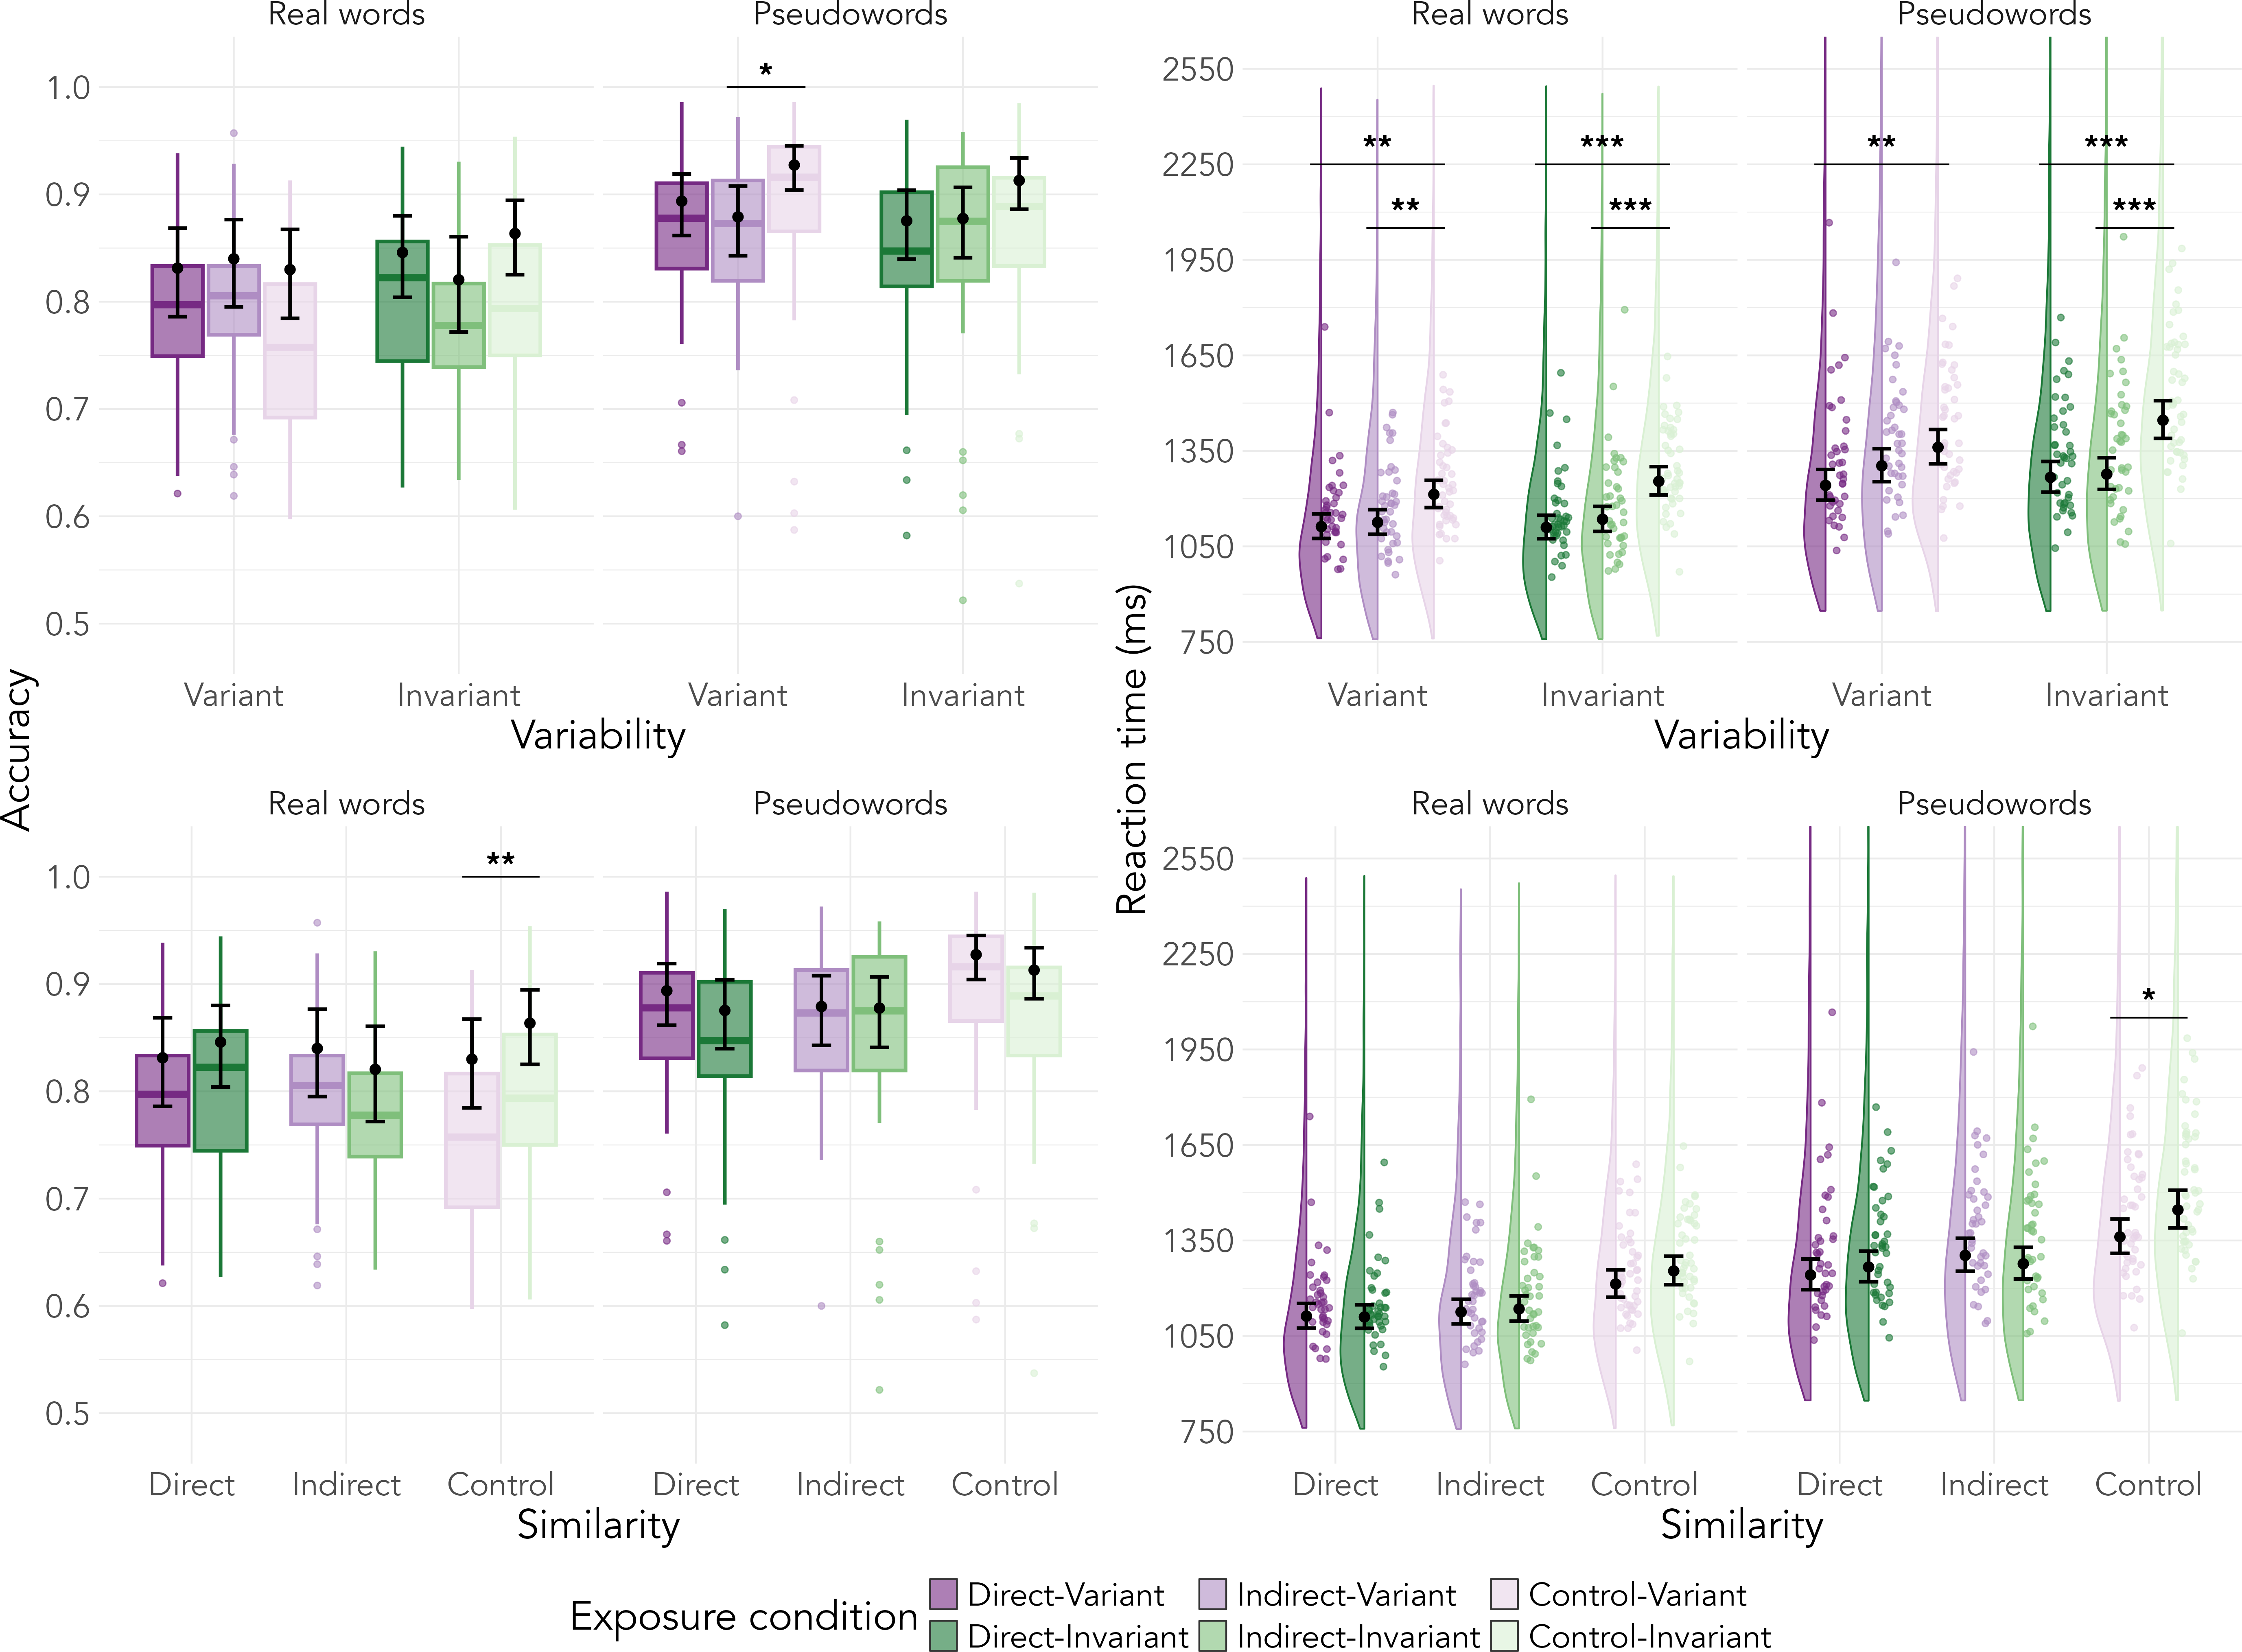
\includegraphics[width=\textwidth]{sections/code/outputs/plot_exp_1a} 

}

\caption{Experiment 1 exposure task performance. Left column presents boxplots with mean accuracy by participant. Right column presents half violin plots with reaction times for correct responses and dot plots with mean reaction times for correct responses by participant. Plots are overlaid with estimated marginal means and 95\% confidence intervals. Asterisks indicate significance levels from pairwise comparisons: *** < .001, ** < .01, * < .05.}\label{fig:exp1-exp-fig}
\end{figure}

\hypertarget{test-comparison-to-the-test-only-group}{%
\subsubsection{Test: Comparison to the Test-only group}\label{test-comparison-to-the-test-only-group}}

For accuracy, we observed a main effect of Exposure (\(\chi^2\)(6, \emph{N} = 7) = 13.28, \emph{p} = .039); however, pairwise comparisons did not reveal significant differences between the Test-only group and any of the exposure groups when averaging across levels of Target (\emph{ps} \textgreater{} .05).
To further investigate the effect of Exposure, we conducted pairwise comparisons between the Test-only group and the exposure groups within each level of Target, but did not observe any significant differences (\emph{ps} \textgreater{} .05).
We also conducted pairwise comparisons between the exposure groups; again, there were no significant differences (\emph{ps} \textgreater{} .05).
By-participant means and estimated marginal means for each level of Exposure and Target are shown in Figure \ref{fig:exp1-test-fig}.

For RT, we observed an interaction between Exposure and Target (\(\chi^2\)(12, \emph{N} = 13) = 24.59, \emph{p} = .017); however, none of the pairwise comparisons between the Test-only group and any of the exposure groups within each level of Target was significant (\emph{ps} \textgreater{} .05).
We also conducted pairwise comparisons between each of the exposure groups, but did not observe any significant differences (\emph{ps} \textgreater{} .05).

\begin{figure}

{\centering 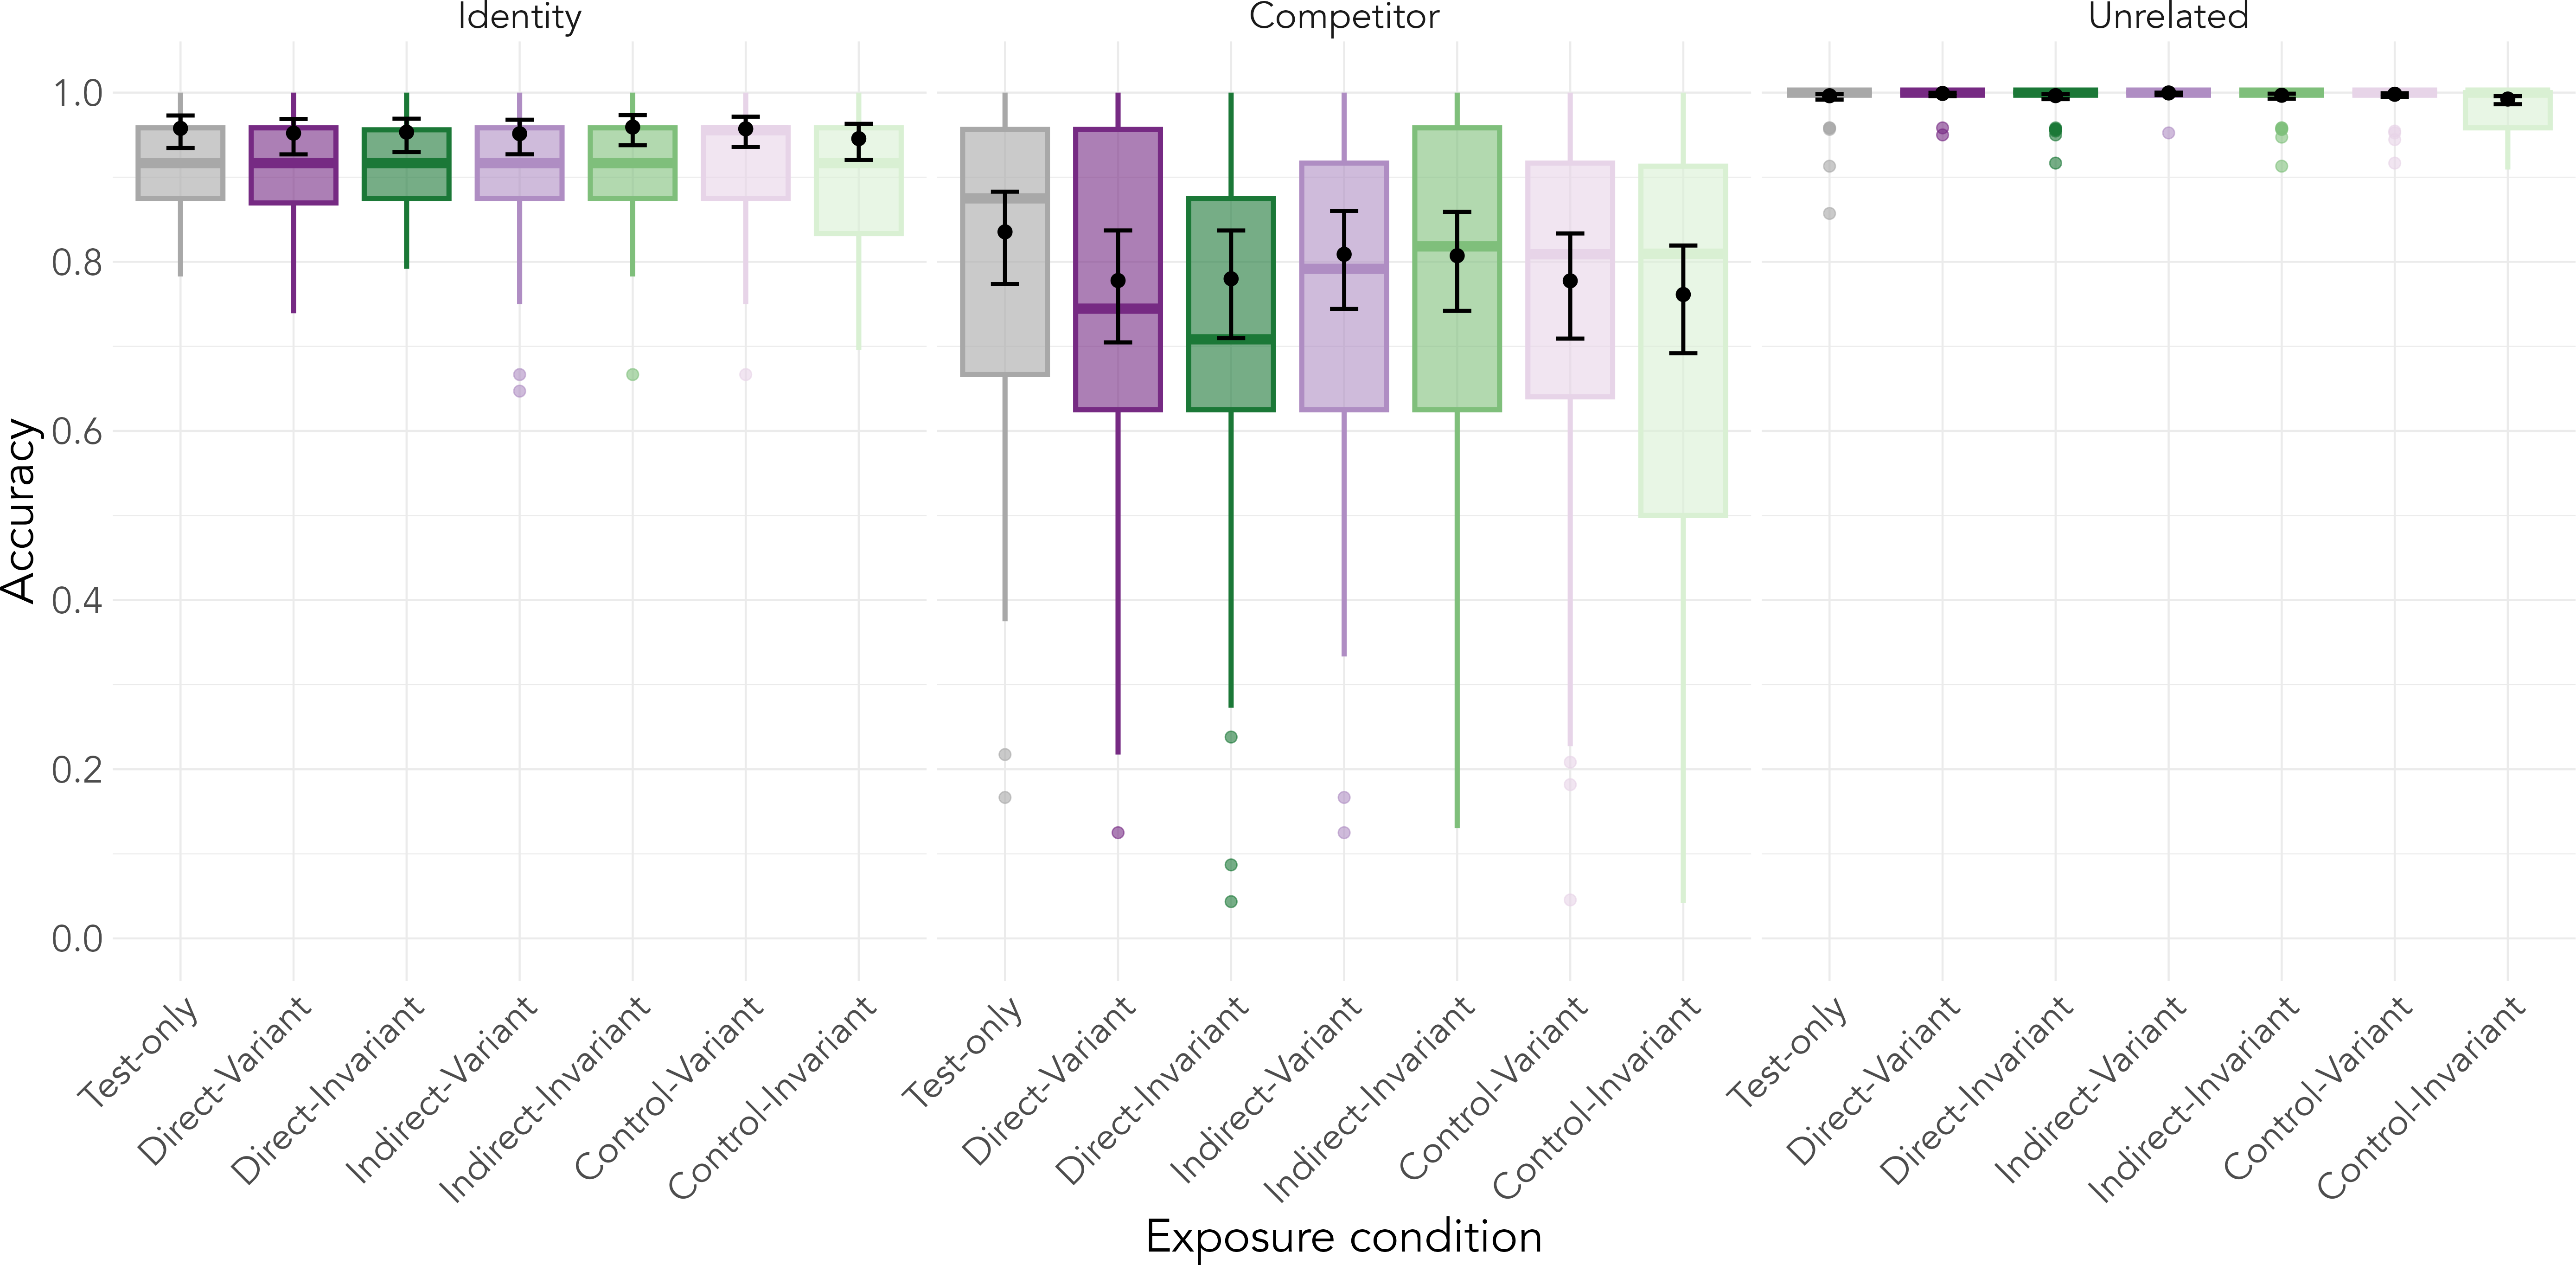
\includegraphics[width=\textwidth]{sections/code/outputs/plot_test_1a} 

}

\caption{Experiment 1 test task accuracy. Boxplots present by-participant means for each Target type. Plots are overlaid with estimated marginal means and 95\% confidence intervals.}\label{fig:exp1-test-fig}
\end{figure}

\hypertarget{discussion}{%
\subsection{Discussion}\label{discussion}}

Experiment 1 compared the effects of exposure to voiceless stops (Direct), voiced stops (Indirect), or voiceless fricatives (Control) on adaptation to Spanish-accented speech.
These three levels of Similarity were crossed with two levels of Variability, such that each talker either produced exemplars of all onsets (Variant) or exemplars of one particular set of onsets (Invariant).
Performance on the exposure task did not differ between the two critical levels of Similarity---Direct and Indirect---in either accuracy or RT.
Between levels of Variability, performance only differed within Control exposure.
The results of the exposure task show that participants were equally able to distinguish real words from pseudowords in the context of Spanish-accented speech regardless of exposure condition.

However, the exposure task did not benefit performance on the test task.
We did not observe differences between the Test-only group, which did not receive any exposure to Spanish-accented speech prior to the test phase, and any of the exposure conditions.
Under the similarity-based hypothesis, we expected Direct exposure to increase accuracy on the matching task, particularly for Competitor targets (\emph{park}-\emph{bark}).
Having direct experience with the mappings between VOT and /p/, /t/, and /k/ in supporting lexical contexts was expected to decrease activation of Competitor targets and increase activation of Identity targets based on \citet{xie2017similarity}.
Here, we observed neither.

A potential difference between our design and that of \citet{xie2017similarity} was in the construction of the pseudowords.
Specifically, we included pseudowords with the experimental onsets that participants were adapting to during exposure.
For example, Direct exposure included both the real word \emph{peanut} and the pseudoword *\emph{pachine}.
While we reasoned in Section \ref{methods-design-1a} that pseudowords like *\emph{pachine} should not disrupt perceptual learning of the relevant VOT-/p/ mapping, it is possible that exposure to these mappings in non-lexical contexts disrupted the benefits of exposure to these mappings in disambiguating lexical contexts.
To address this issue, we removed these pseudowords in Experiment 2.
Instead, participants in the Direct and Indirect groups were both exposed to pseudowords with control onsets like *\emph{fachine}.
Including control onsets within the Direct and Indirect groups lessened the need for separate Control groups.
To reduce the complexity of the design and home in on the effects of Direct versus Indirect exposure, the Control level of Similarity was not included in Experiment 2.

\hypertarget{experiment-2-investigating-the-specificity-of-generalization-from-exposure-to-spanish-accented-stops}{%
\section{Experiment 2: Investigating the specificity of generalization from exposure to Spanish-accented stops}\label{experiment-2-investigating-the-specificity-of-generalization-from-exposure-to-spanish-accented-stops}}

\hypertarget{methods-1}{%
\subsection{Methods}\label{methods-1}}

This experiment was the same as Experiment 1, with the exception of the Similarity factor.

\hypertarget{design}{%
\subsubsection{Design}\label{design}}

The Control level was removed, leaving just two levels of Similarity: Direct and Indirect.
Recall that the pseudowords in the Direct and Indirect conditions had the same onsets as the experimental real words (critical and competitor, respectively).
It is possible that this design disrupted adaptation to Spanish-accented VOTs by associating them with pseudowords.
To improve learning, we replaced them with pseudowords with control onsets.

\begin{figure}

{\centering 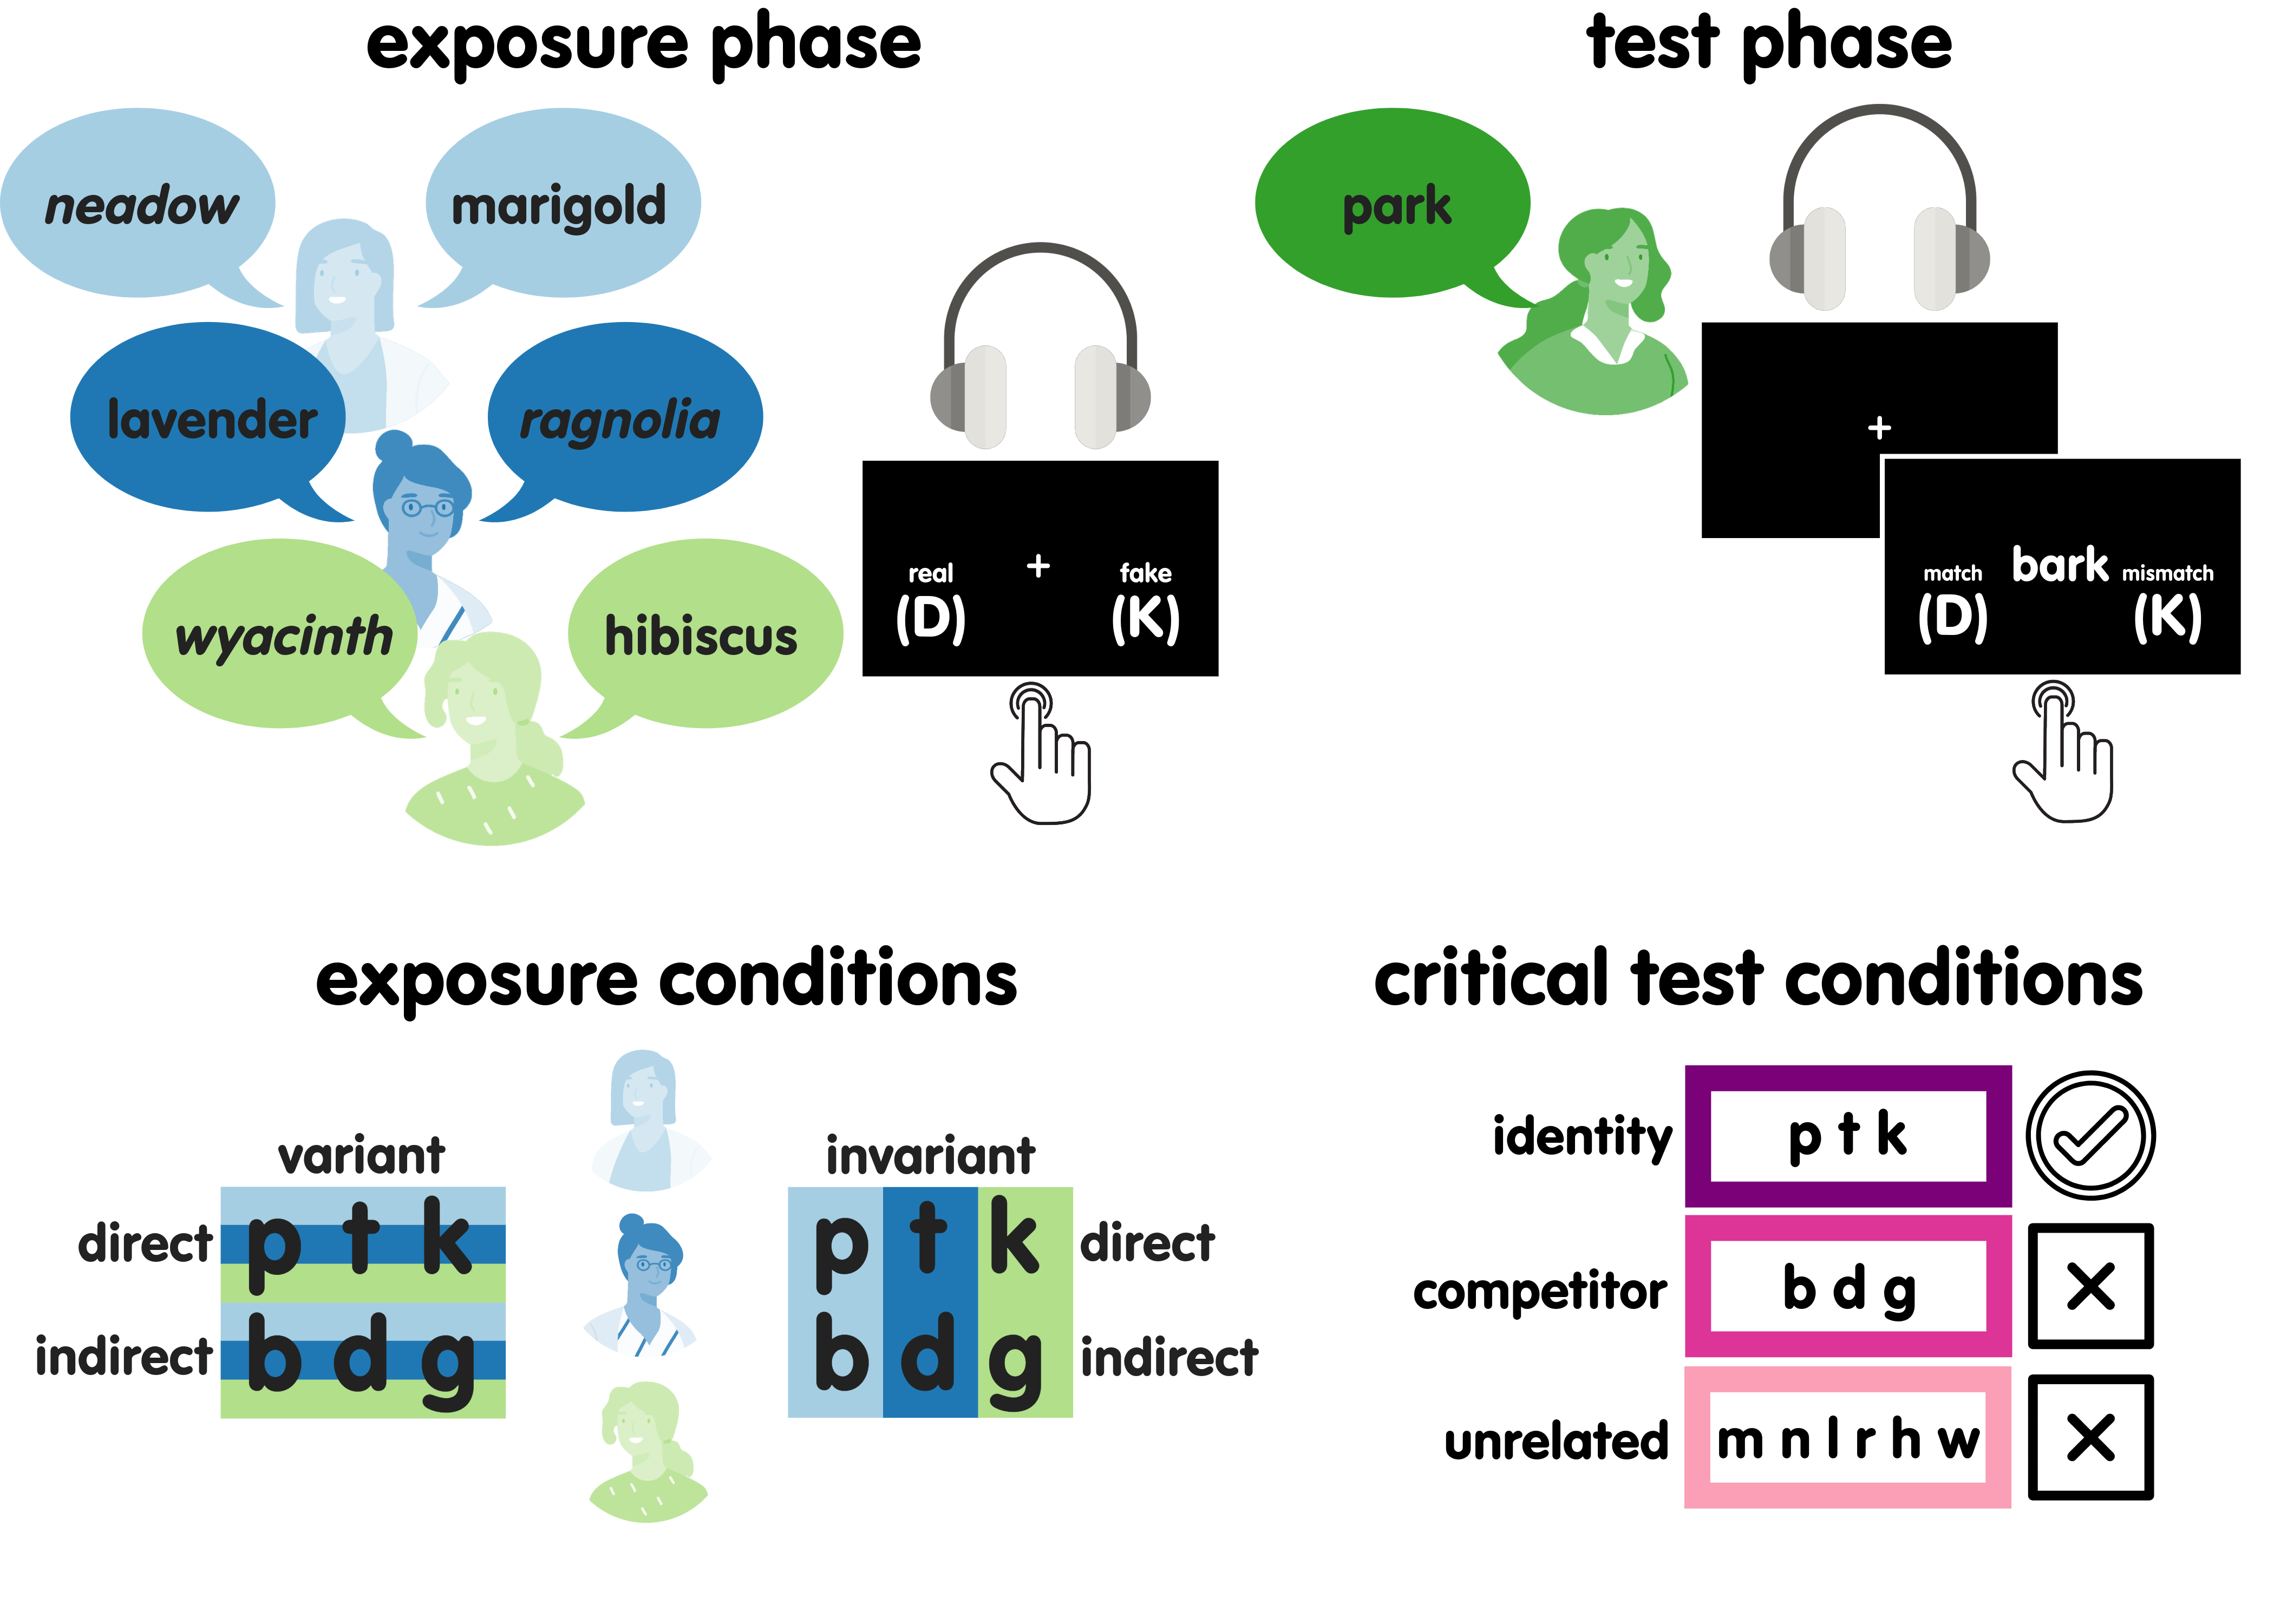
\includegraphics[width=\textwidth]{../14_final_diss/figures/diss_2} 

}

\caption{Experiment 2 design.}\label{fig:exp2-fig}
\end{figure}

\hypertarget{methods-pars-1b}{%
\subsubsection{Participants}\label{methods-pars-1b}}

We recruited 192 participants through Prolific, none of whom had participated in Experiment 1.
All aspects of recruitment and criteria for data exclusion were the same as in Experiment 1.
After removing ineligible participants, 160 remained.
After removing participants with poor data quality, 154 remained for analysis (Age: \emph{M} = 31, \emph{SD} = 6, Min = 18, Max = 40; Sex: Female = 65, Male = 89; Race: Asian = 5, Black = 17, Multiple selected = 12, Other = 4, White = 116).
Data from the participants who completed the experiment without the exposure phase in Experiment 1 were used for comparison.

\hypertarget{materials-and-procedure}{%
\subsubsection{Materials and procedure}\label{materials-and-procedure}}

The talkers, stimuli, tasks, and procedure were the same as those in Experiment 1.
Removing the Control level of Similarity from the exposure phase left four between-subjects conditions: Direct-Variant, Direct-Invariant, Indirect-Variant, and Indirect-Invariant.
The 288 filler items remained the same.
The 72 experimental real words also remained the same.
The 72 experimental pseudowords had control onsets regardless of Similarity.
Talker assignment and counterbalancing was the same.
This resulted in 16 experimental lists for the exposure phase, one for each combination of exposure condition (4) and talker assignment (4).
All aspects of the test phase remained the same.

\hypertarget{analysis-and-predictions}{%
\subsubsection{Analysis and predictions}\label{analysis-and-predictions}}

The data processing, model fitting, and analysis approaches were the same as in Experiment 1; the only change was implementing sum contrasts for the two levels of Similarity.
Prior to analyzing exposure task performance for real words with experimental onsets, we removed responses with RTs less than 50 ms (\emph{N} = 64; 0.10\%).
We then detected and removed outliers (\emph{N} = 2917; 4.39\%).
Prior to analyzing test task performance for critical prime-target pairs, we removed responses with RTs less than 50 ms (\emph{N} = 7; 0.05\%).
We then detected and removed outliers (\emph{N} = 679; 4.94\%).

\hypertarget{results-1}{%
\subsection{Results}\label{results-1}}

\hypertarget{exposure-1}{%
\subsubsection{Exposure}\label{exposure-1}}

For accuracy, we observed significant interactions among Variability, Similarity, and Word type (\(\chi^2\)(1, \emph{N} = 2) = 10.78, \emph{p} = .001) and between Variability and Word type (\(\chi^2\)(1, \emph{N} = 2) = 4.64, \emph{p} = .031).
To investigate these effects, we conducted pairwise comparisons between levels of Similarity within each combination of Variability and Word type and between levels of Variability within each combination of Similarity and Word type.
These comparisons are shown in the left column of Figure \ref{fig:exp2-exp-fig}.
Within Variant exposure, pseudoword accuracy was higher for Direct exposure (\emph{M} = 0.91, 95\% CI {[}0.88, 0.93{]}) compared to Indirect exposure (\emph{M} = 0.94, 95\% CI {[}0.92, 0.95{]}; \emph{z} = 2.80, \emph{p} = .005).

For RT, the interaction between Variability and Word type was significant (\(\chi^2\)(1, \emph{N} = 2) = 10.66, \emph{p} = .001).
Pairwise comparisons between Variant and Invariant exposure within each level of Word type were not significant (\emph{ps} \textgreater{} .05).
To further explore the effects of Variability and Similarity on RTs, we also conducted the same pairwise comparisons as we did for accuracy; however, there were no differences in this case (\emph{ps} \textgreater{} .05).
These comparisons are shown in the right column of Figure \ref{fig:exp2-exp-fig}.

\begin{figure}

{\centering 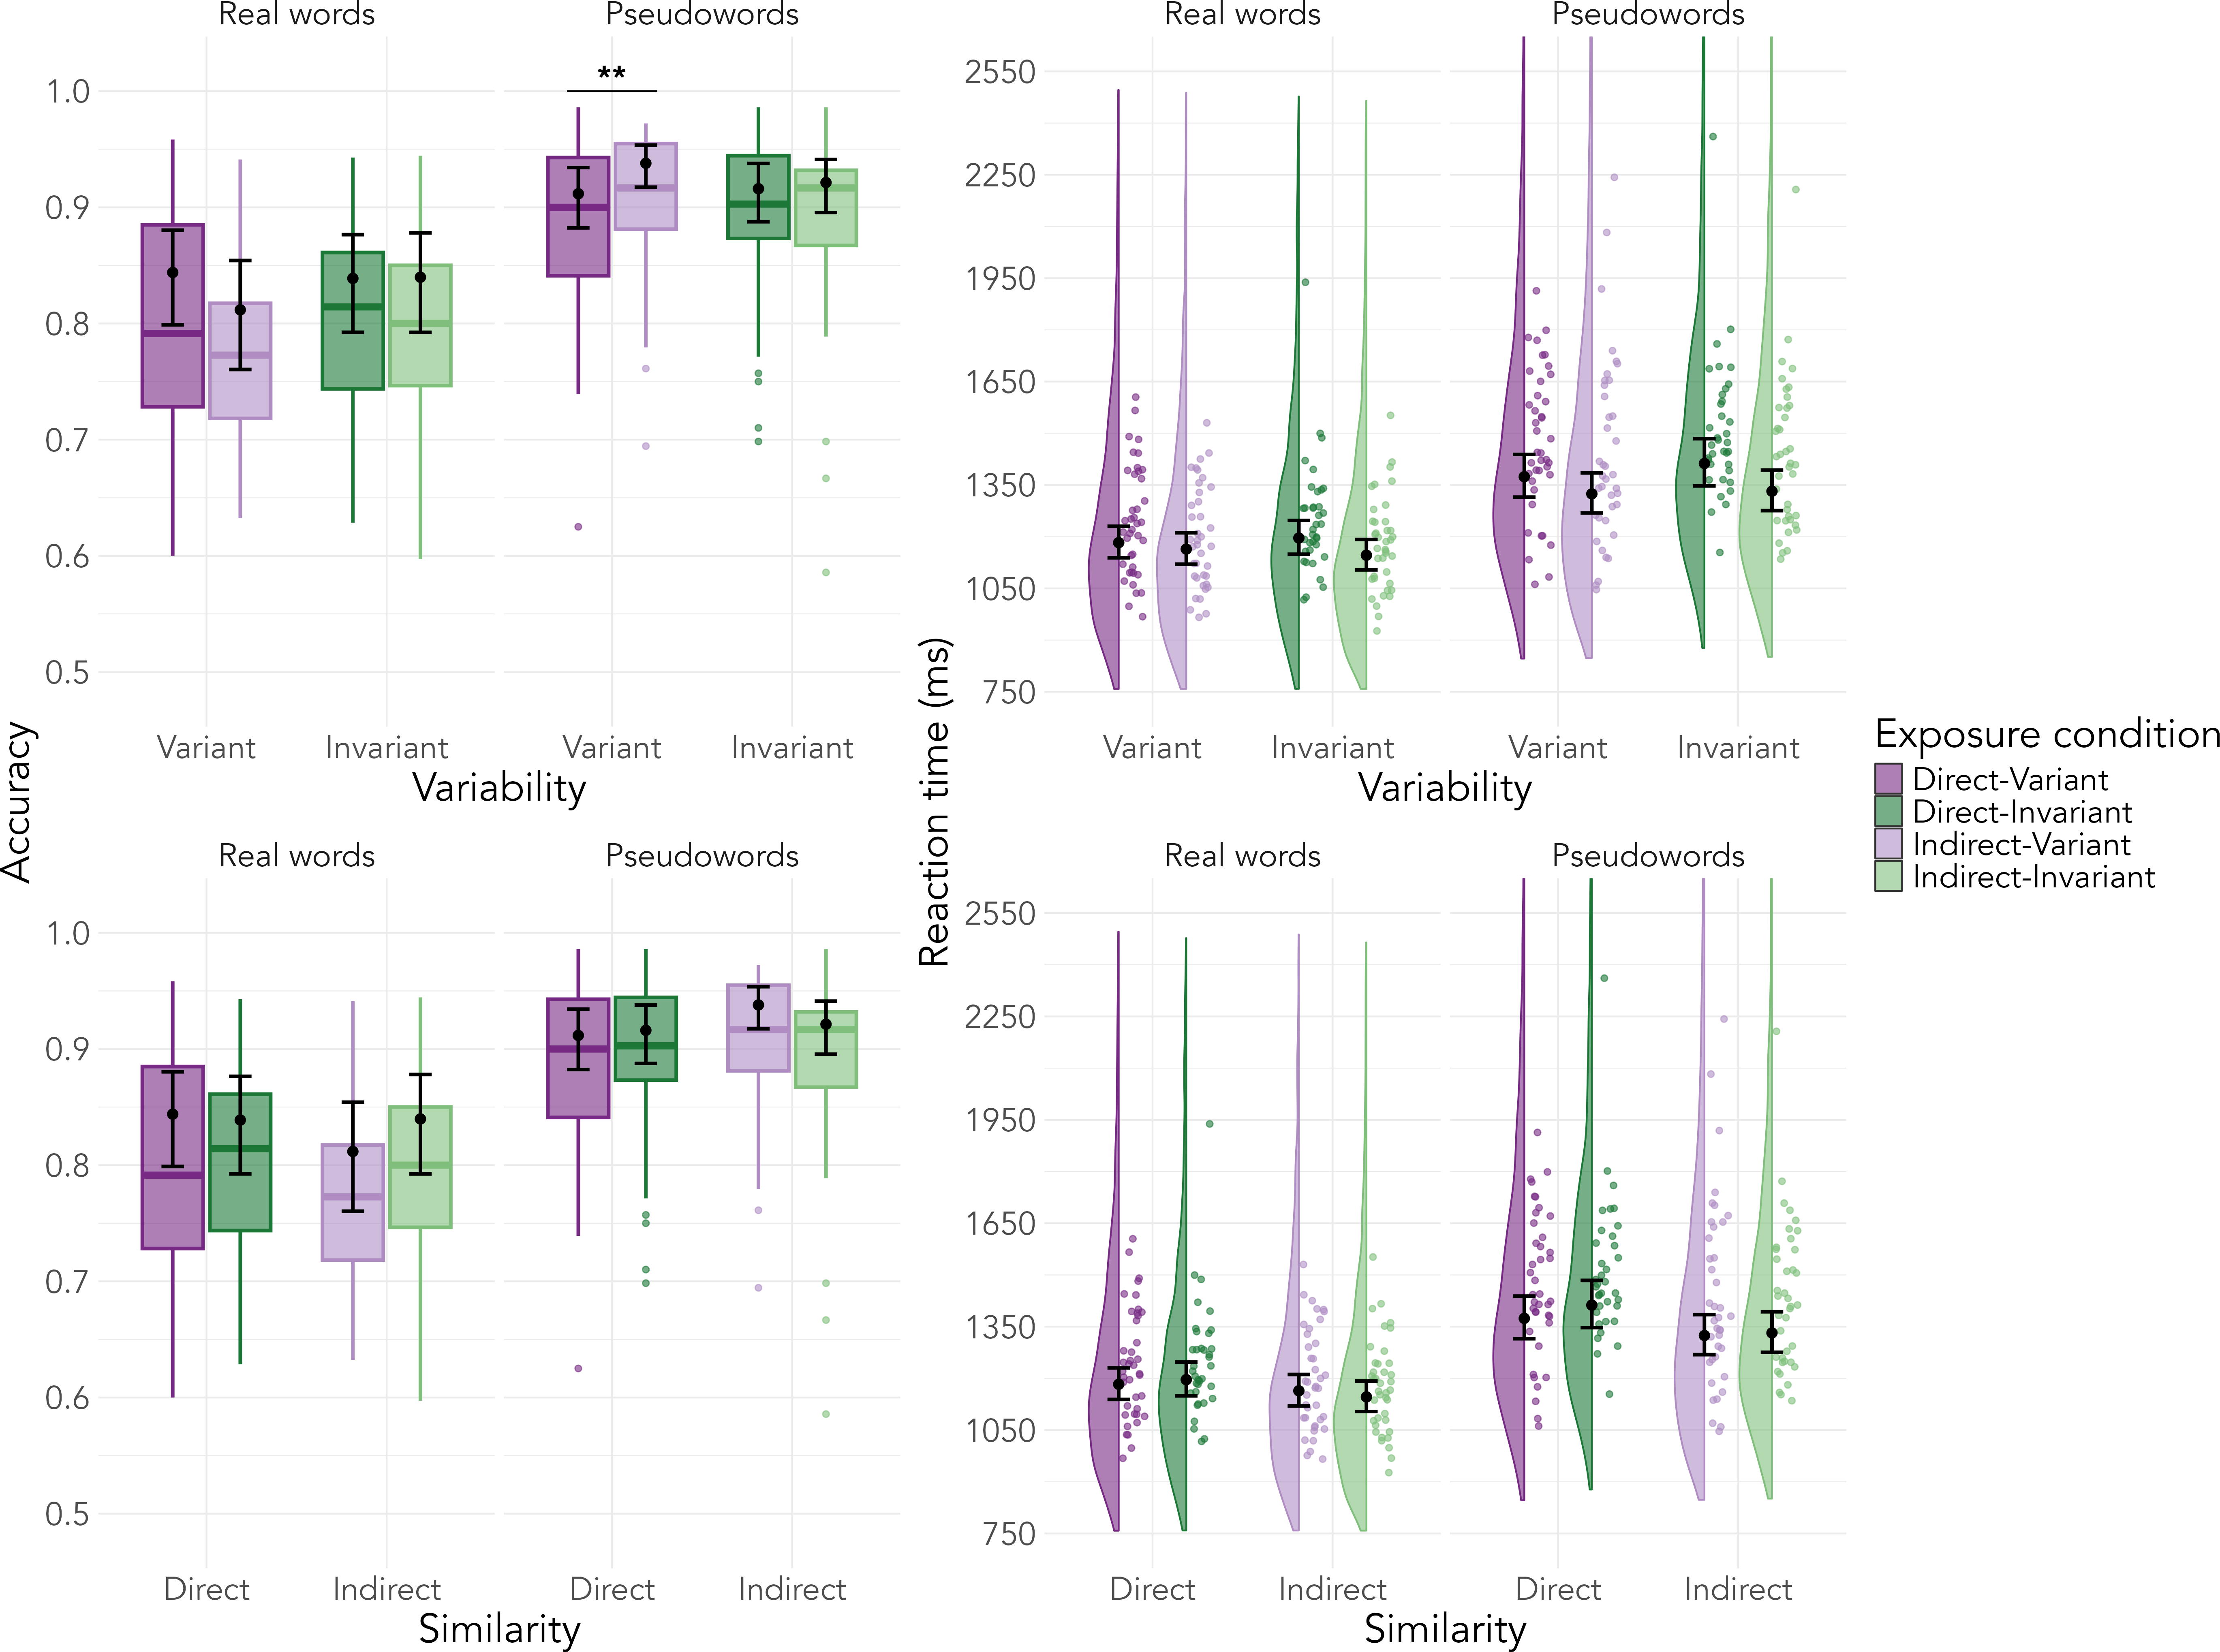
\includegraphics[width=\textwidth]{sections/code/outputs/plot_exp_1b} 

}

\caption{Experiment 2 exposure task performance. Left column presents boxplots with mean accuracy by participant. Right column presents half violin plots with reaction times for correct responses and dot plots with mean reaction times for correct responses by participant. Plots are overlaid with estimated marginal means and 95\% confidence intervals. Asterisks indicate significance levels from pairwise comparisons: *** < .001, ** < .01, * < .05.}\label{fig:exp2-exp-fig}
\end{figure}

\hypertarget{test-comparison-to-the-test-only-group-1}{%
\subsubsection{Test: Comparison to the Test-only group}\label{test-comparison-to-the-test-only-group-1}}

For accuracy, we observed a significant interaction between Exposure and Target (\(\chi^2\)(8, \emph{N} = 9) = 20.20, \emph{p} = .010).
Pairwise comparisons within each level of Target did not reveal significant differences between the Test-only group and any of the exposure groups (\emph{ps} \textgreater{} .05).
To investigate the source of the Exposure-Target interaction, we conducted pairwise comparisons between each of the exposure groups
Direct-Invariant exposure yielded significantly higher accuracy on Competitor targets (\emph{M} = 0.87, 95\% CI {[}0.82, 0.91{]}) than Direct-Variant exposure (\emph{z} = 2.99, \emph{p} = .017), Indirect-Invariant exposure (\emph{z} = 2.68, \emph{p} = .030), or Indirect-Variant exposure (\emph{z} = 2.55, \emph{p} = .043).
By-participant means and estimated marginal means are shown in Figure \ref{fig:exp2-test-fig}.

For RT, we also observed a significant interaction between Exposure and Target (\(\chi^2\)(8, \emph{N} = 9) = 41.53, \emph{p} \textless{} .001).
Pairwise comparisons within each level of Target did not reveal significant differences between the Test-only group and any of the exposure groups (\emph{ps} \textgreater{} .05).
Pairwise comparisons between the exposure groups revealed significantly slower RTs on Identity targets for Direct-Invariant exposure (\emph{M} = 0.95, 95\% CI {[}0.92, 0.97{]}) than for Indirect-Variant exposure (\emph{M} = 0.95, 95\% CI {[}0.93, 0.97{]}; \emph{z} = 2.79, \emph{p} = .032).

\begin{figure}

{\centering 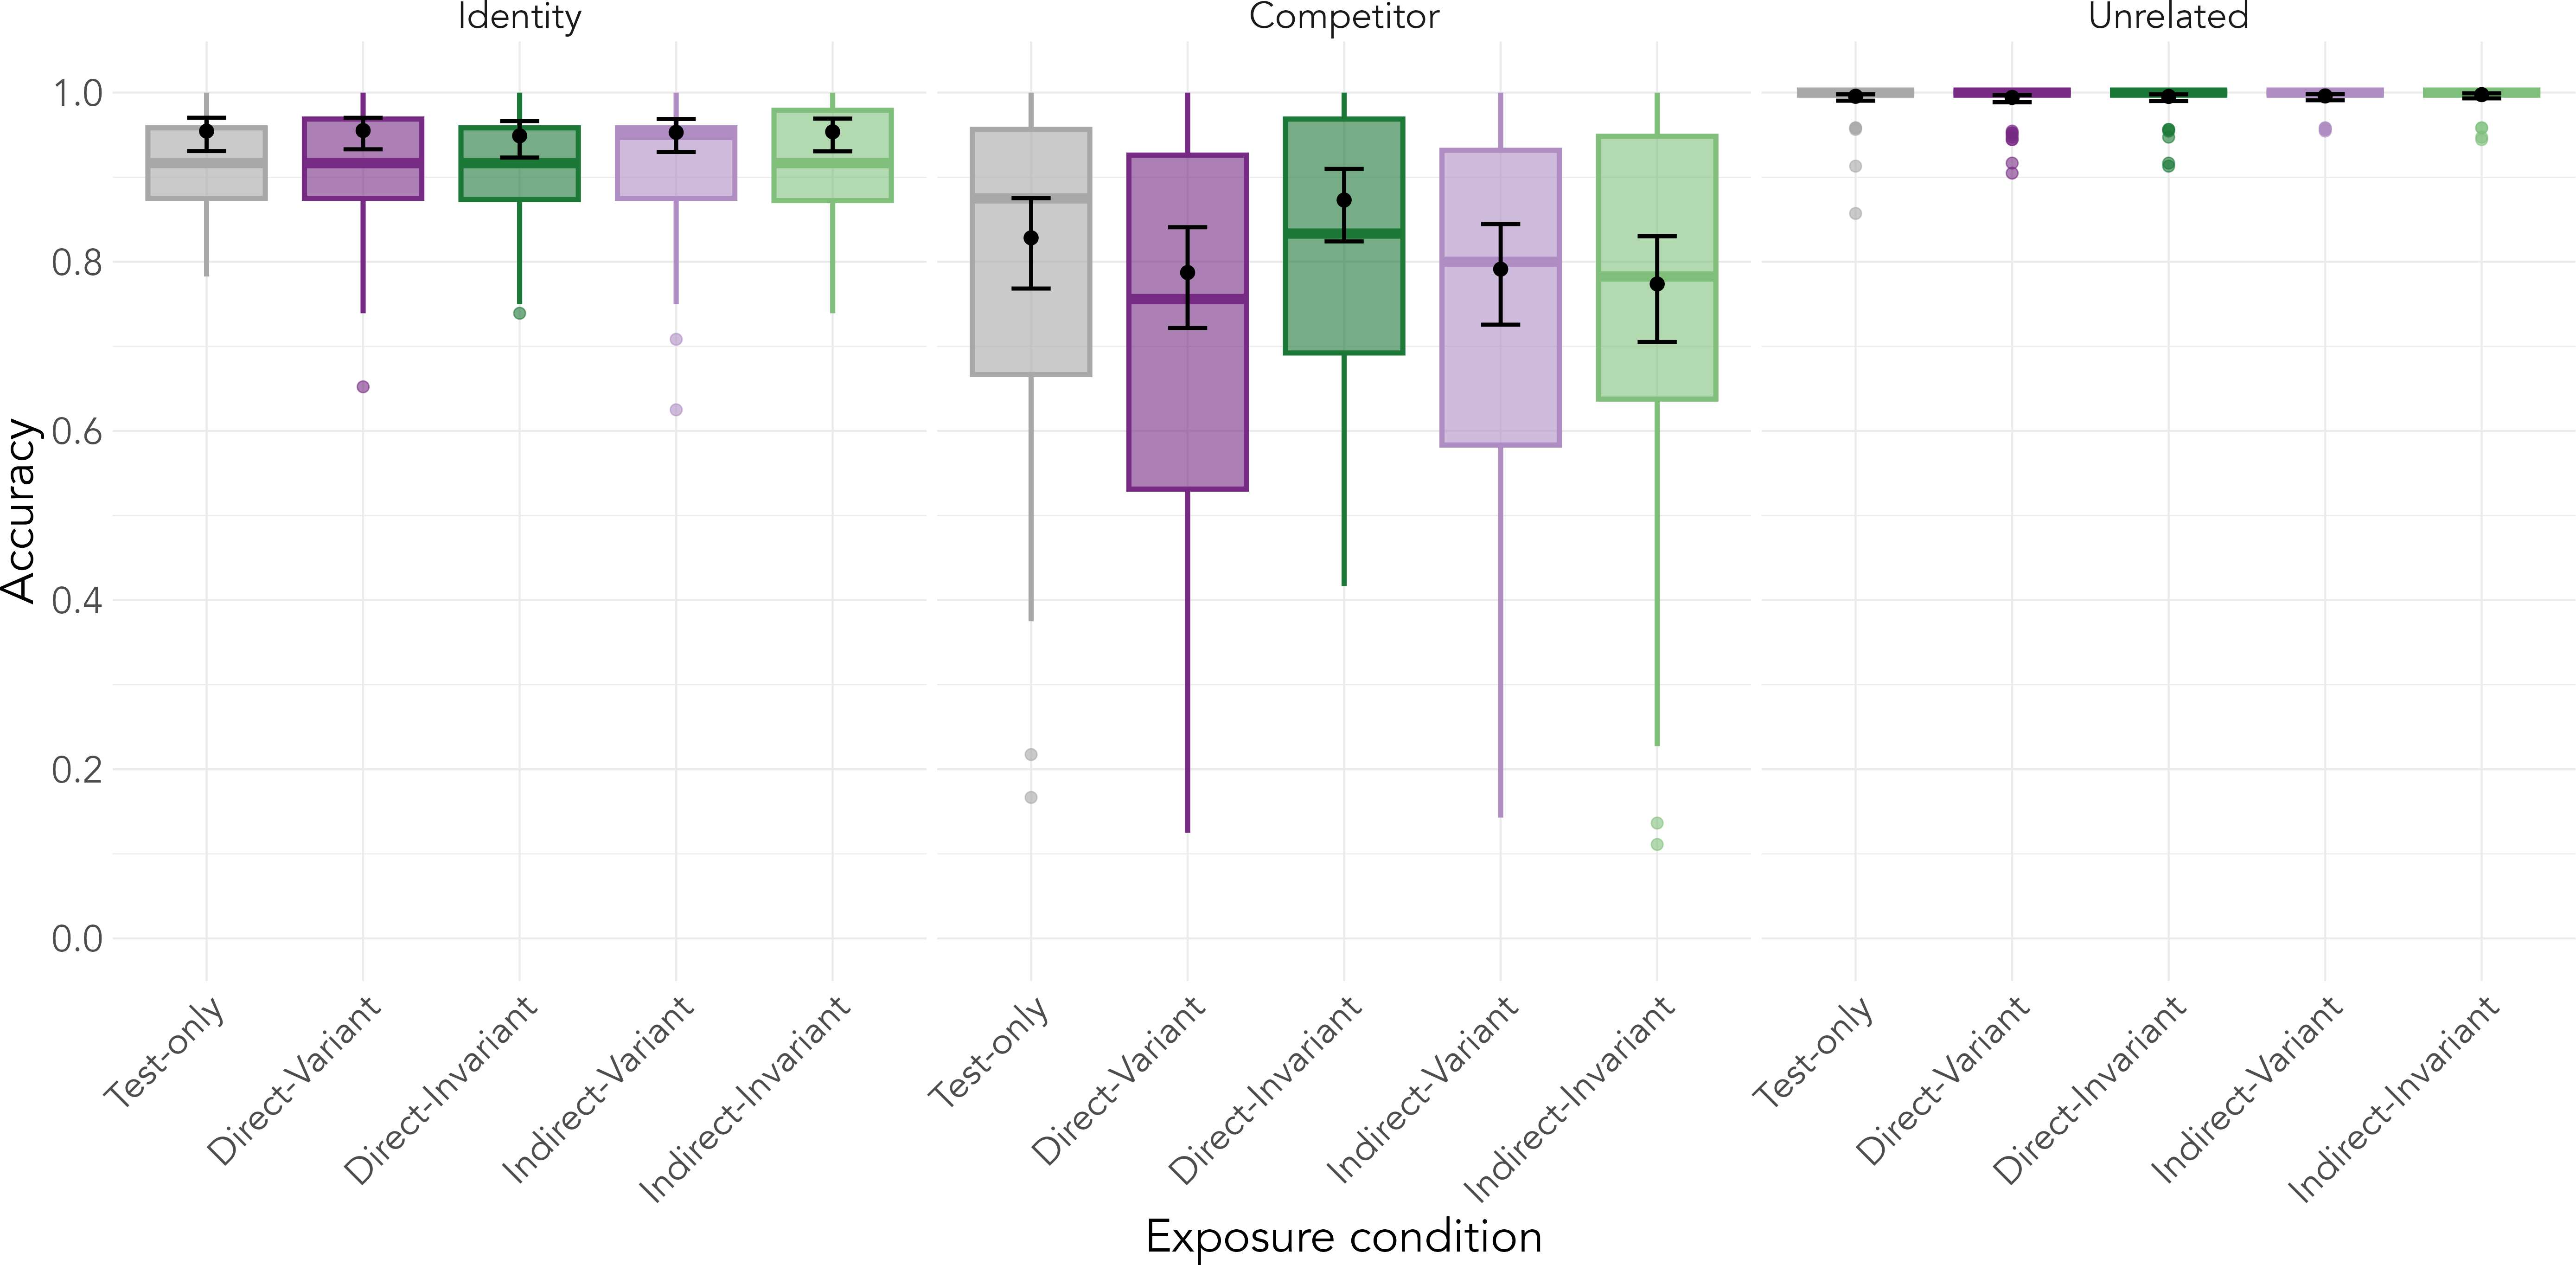
\includegraphics[width=\textwidth]{sections/code/outputs/plot_test_1b} 

}

\caption{Experiment 2 test task accuracy. Boxplots present by-participant means for each Target type. Plots are overlaid with estimated marginal means and 95\% confidence intervals.}\label{fig:exp2-test-fig}
\end{figure}

\hypertarget{discuss-1b}{%
\subsection{Discussion}\label{discuss-1b}}

In Experiment 2, two levels of Similarity---Direct and Indirect---were crossed with two levels of Variability---Variant and Invariant---in order to investigate how experience with Spanish-accented stops transfers to a novel talker.
During the exposure task, participants performed equally well across conditions.
The only difference we observed was on pseudoword accuracy, where the Indirect-Variant group outperformed the Direct-Variant group.
Overall, the results of the exposure task suggest that word recognition in Spanish-accented speech was successful regardless of Similarity or Variability.

As in Experiment 1, the exposure task did not benefit performance on the test task.
Compared to the Test-only group, none of the exposure groups performed differently.
However, we did observe differences between exposure groups.
Specifically, the Direct-Invariant group was more accurate on Competitor targets than any of the other three exposure groups.
This group was also slower on Identity targets than the Indirect-Variant group.

In order to interpret these findings in terms of generalization, we will briefly describe the structure of the exposure conditions again.
Both Direct conditions exposed participants to Spanish-accented /p/, /t/, and /k/ in such disambiguating lexical contexts as \emph{peanut}, \emph{terminal}, and \emph{kingdom}, respectively.
However, the Direct-Invariant condition in particular exposed participants to one-to-one mappings between each critical onset and each talker, such that all /p/ onsets were produced by Talker A, all /t/ onsets by Talker B, and all /k/ onsets by Talker C.
Thus, participants in the Direct-Invariant group were given the opportunity to develop talker-specific generative models for each VOT-stop mapping.
Recall that a generative model refers to a listener's mental representation of the distribution of a phonetic category (like /p/) over an acoustic cue (like VOT) under the ideal adapter framework.
Since generative models are specific to pairs of cues and categories under this theory, listeners in the Invariant conditions had to organize their representations of VOT for each onset by talker.
By contrast, listeners in the Variant conditions had the option to integrate across talkers to organize each VOT-stop mapping at the accent level, since all three talkers produced exemplars of all onsets.
The high performance of the Direct-Invariant group on Competitor targets suggests that robust talker-specific generative models for voiceless stops may reduce the (erroneous) activation of voiced stops in response to Spanish-accented primes like \emph{park}.
The slight reduction in performance for this group on Identity targets suggests that such generative models may not increase the activation of voiceless stops in turn.
Together, these findings suggest that exposure-test similarity is necessary but not sufficient for talker-independent perceptual adaptation.

Finally, we return to the lack of significant differences between the Test-only and Direct-Invariant groups.
The fact that participants without exposure were able to perform at a similar level to those with exposure weakens the argument we put forward in the previous paragraph.
If exposure facilitates generalization, but generalization does not facilitate future performance, then what is the benefit of exposure?
However, there is a wealth of evidence that previous exposure to an L2 accent improves perception of a novel L2-accented talker with the same L1 \citep{bent2021}.
Previous studies have generally used either sentence transcription \citep[e.g.,][]{bradlow2008} or primed lexical decision \citep[e.g.,][]{xie2017similarity} to test the strength of adaptation.
Here, we used a matching task, under the assumption that categorization of short lag VOTs as voiceless stops should change as a function of perception of short lag VOTs as voiceless stops.
For example, consider the auditory prime \emph{park} and the visual target \emph{bark}.
Participants needed to decide whether the onset of the token they had heard was a /b/ or not.
If they accurately perceived the onset as a /p/, then they would correctly reject \emph{bark} as a match.
Thus, accuracy on the matching task was the outcome of the categorization process.
It is possible that this outcome-based measure was not fine-grained enough to capture subtle changes in perception.
To return to the Competitor target example, the lack of difference in categorizing Spanish-accented \emph{park} as \emph{bark} may belie differences in perceiving Spanish-accented /p/.
To better assess changes in perception, we changed the test task for Experiment 3.

\hypertarget{experiment-3-investigating-fine-grained-perceptual-changes-from-exposure-to-spanish-accented-stops}{%
\section{Experiment 3: Investigating fine-grained perceptual changes from exposure to Spanish-accented stops}\label{experiment-3-investigating-fine-grained-perceptual-changes-from-exposure-to-spanish-accented-stops}}

\hypertarget{methods-2}{%
\subsection{Methods}\label{methods-2}}

The exposure phase was the same as Experiment 2, but the task used in the test phase was different.

\hypertarget{design-1}{%
\subsubsection{Design}\label{design-1}}

To better detect subtle changes in perception as a function of exposure to Spanish-accented speech, we implemented the primed cross-modal lexical decision task from \citet{xie2017similarity}.
This design is illustrated in Figure \ref{fig:exp3-fig}.
We maintained the same three types of Target: Identity, Competitor, and Unrelated.
However, participants performed a different task with these targets relative to Experiment 2.
Specifically, participants decided whether the visual target was a real English word or not.
The auditory primes should increase or decrease RTs on the visual targets as a function of perceptual adaptation to Spanish-accented voiceless stops.

\begin{figure}

{\centering 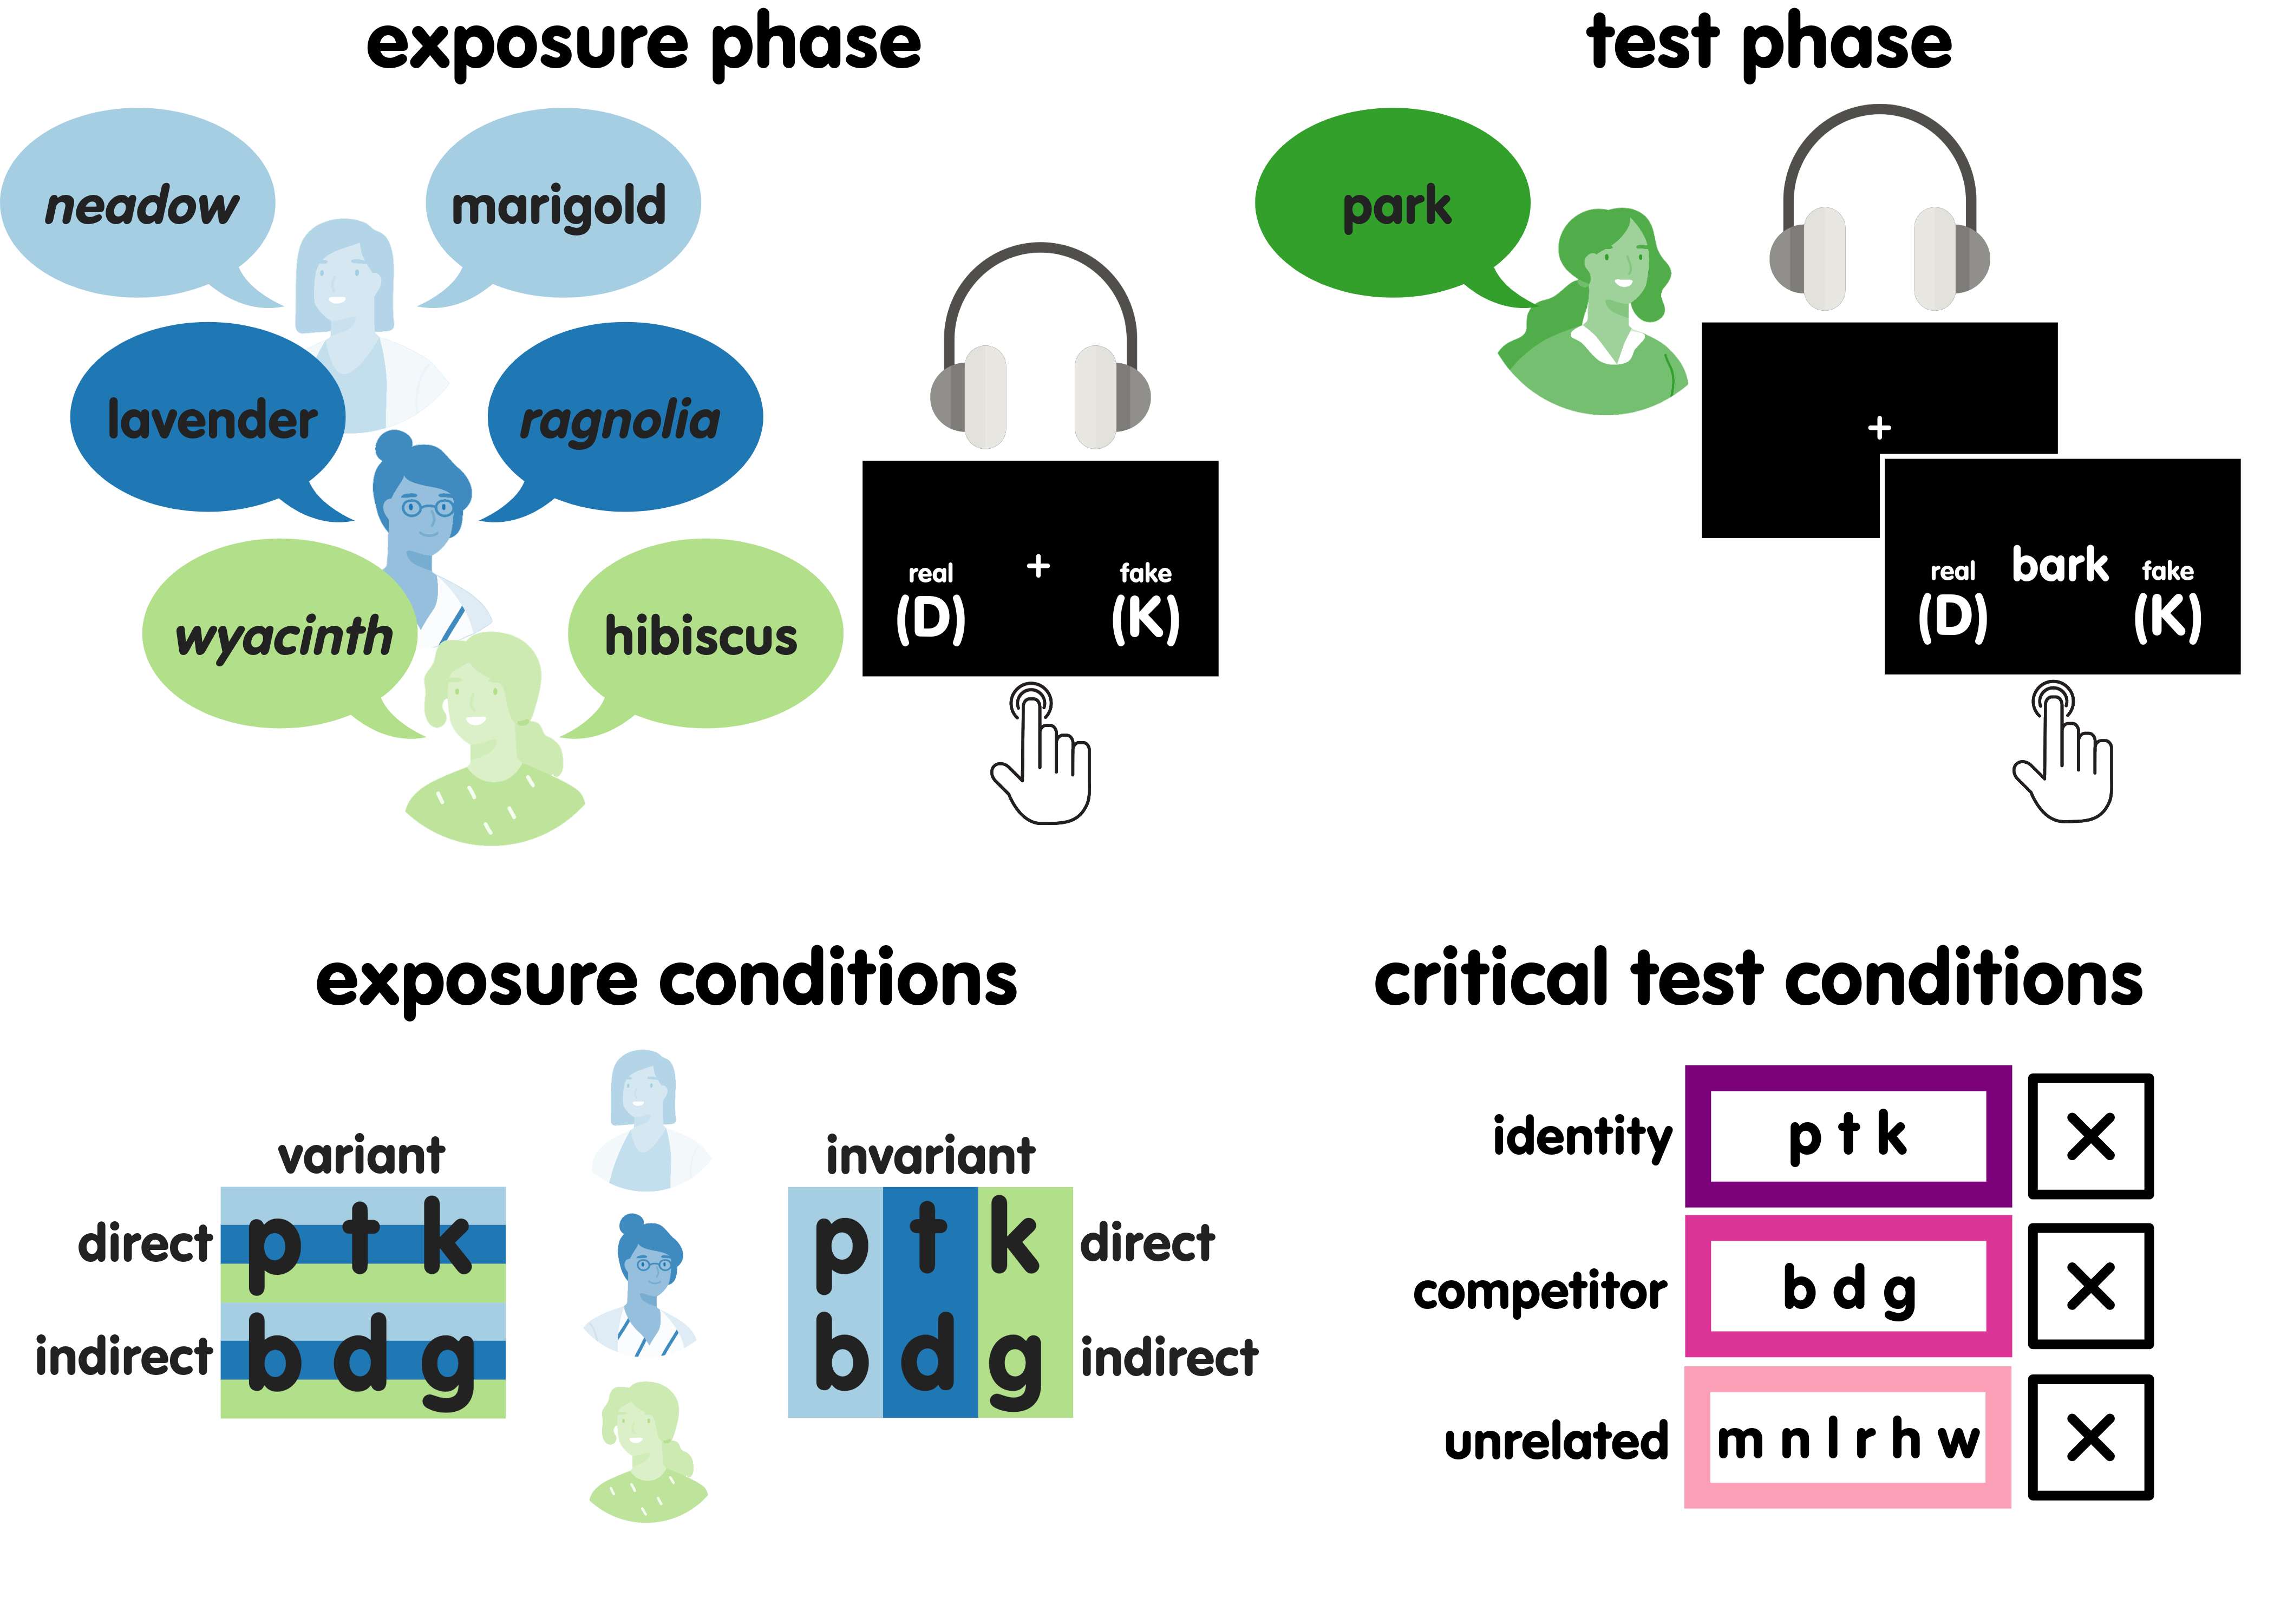
\includegraphics[width=\textwidth]{../14_final_diss/figures/diss_3} 

}

\caption{Experiment 3 design.}\label{fig:exp3-fig}
\end{figure}

\hypertarget{methods-pars-2}{%
\subsubsection{Participants}\label{methods-pars-2}}

We recruited 195 participants through Prolific; none had participated in Experiments 1 or 2.
All aspects of recruitment and criteria for data exclusion were the same as in Experiments 1 and 2.
After removing ineligible participants, 170 remained.
After removing participants with poor data quality, 158 remained for analysis (Age: \emph{M} = 31, \emph{SD} = 6, Min = 18, Max = 40; Sex: Female = 80, Male = 78; Race: Asian = 4, Black = 20, Multiple selected = 13, Other = 4, White = 117).

Additionally, a new group of 50 participants was also recruited to complete the experiment without the exposure phase.
There were 43 participants remaining after checking the eligibility criteria, and 42 participants remained after checking for data quality (Age: \emph{M} = 30, \emph{SD} = 5, Min = 21, Max = 40; Sex: Female = 20, Male = 22; Race: Black = 3, Multiple selected = 5, White = 34).

\hypertarget{stimuli}{%
\subsubsection{Stimuli}\label{stimuli}}

The real words and pseudowords in the exposure task were the same as those in Experiment 2.
The auditory primes in the test task were also the same.
The only difference was in the visual targets.

The unrelated target for each filler prime (144) was replaced with a pseudoword with a different filler onset from the prime.
Potential pseudowords were downloaded from the ELP's set of normed pseudowords.
The best possible match was selected for each prime by (orthographic) vowel and number of letters.
Three additional pseudoword targets were selected for practice.

\hypertarget{experimental-lists}{%
\subsubsection{Experimental lists}\label{experimental-lists}}

The experimental lists for the exposure task were the same as in Experiment 2.
Talker assignment was also counterbalanced the same way.

For the critical primes (72), the combinations of auditory prime and visual target were counterbalanced across participants in three experimental lists as in Experiment 2.
For the filler primes (144), perfect counterbalancing across these three lists was not possible, since three quarters of the filler items in each list (108) needed to have unrelated pseudoword targets.
Three sets of primes, divided evenly by onset, were rotated through the assignment of Identity or Unrelated (pseudoword) target as evenly as possible.
This resulted in 12 experimental lists for the test phase, one for each combination of critical prime-target pair (3) and talker assignment (4).

\hypertarget{tasks-and-procedure}{%
\subsubsection{Tasks and procedure}\label{tasks-and-procedure}}

The headphone check, exposure task, and post-experiment questionnaire were the same as Experiment 2.
The procedure was also the same.
The only difference was in the structure of the test task.

The test phase featured the cross-modal primed lexical decision task from \citet{xie2017similarity}.
On each trial, participants first heard a real word (auditory prime) and then saw a real word or pseudoword written on the screen (visual target).
They indicated whether the visual target was a real English word or not by pressing the \emph{d} or \emph{k} key on their keyboard.
The real word response was mapped to the same key as in the exposure task.
Participants completed six practice trials followed by 216 main trials presented in random order.
Half of the practice trials (3) and half of the main trials (108) required real word responses.
All of the trials with critical primes (72) required real word responses.

\hypertarget{analysis}{%
\subsubsection{Analysis}\label{analysis}}

The data processing, model fitting, and analysis approaches were the same as in Experiment 2.
Prior to analyzing exposure task performance for real words with experimental onsets, we removed responses with RTs less than 50 ms (\emph{N} = 22; 0.03\%).
We then detected and removed outliers (\emph{N} = 2953; 4.33\%).
Prior to analyzing test task performance for critical prime-target pairs, we removed responses with RTs less than 50 ms (\emph{N} = 53; 0.37\%).
We then detected and removed outliers (\emph{N} = 1076; 7.50\%).

\hypertarget{results-2}{%
\subsection{Results}\label{results-2}}

\hypertarget{exposure-2}{%
\subsubsection{Exposure}\label{exposure-2}}

For accuracy, there was a significant interaction between Variability and Word type (\(\chi^2\)(1, \emph{N} = 2) = 17.77, \emph{p} \textless{} .001), with higher accuracy on pseudowords in Variant groups (\emph{M} = 0.94, 95\% CI {[}0.92, 0.95{]}) compared to Invariant groups (\emph{M} = 0.92, 95\% CI {[}0.90, 0.94{]}; \emph{z} = 2.63, \emph{p} = .009).
We also conducted pairwise comparisons within each combination of Similarity and Word type and within each combination of Variability and Word type.
There were no significant effects of Variability or Similarity, respectively (\emph{ps} \textgreater{} .05).
These comparisons are shown in the left column of Figure \ref{fig:exp3-exp-fig}.

For RT, there was a significant three-way interaction among Variability, Similarity, and Word type (\(\chi^2\)(1, \emph{N} = 2) = 9.11, \emph{p} = .003).
The two-way interaction between Similarity and Word type was also significant (\(\chi^2\)(1, \emph{N} = 2) = 4.40, \emph{p} = .036).
To follow up on the three-way interaction, we analyzed the simple effects of Variability and Similarity; however, none of the pairwise comparisons was significant (\emph{ps} \textgreater{} .05).
These comparisons are shown in the right column of Figure \ref{fig:exp3-exp-fig}.

\begin{figure}

{\centering 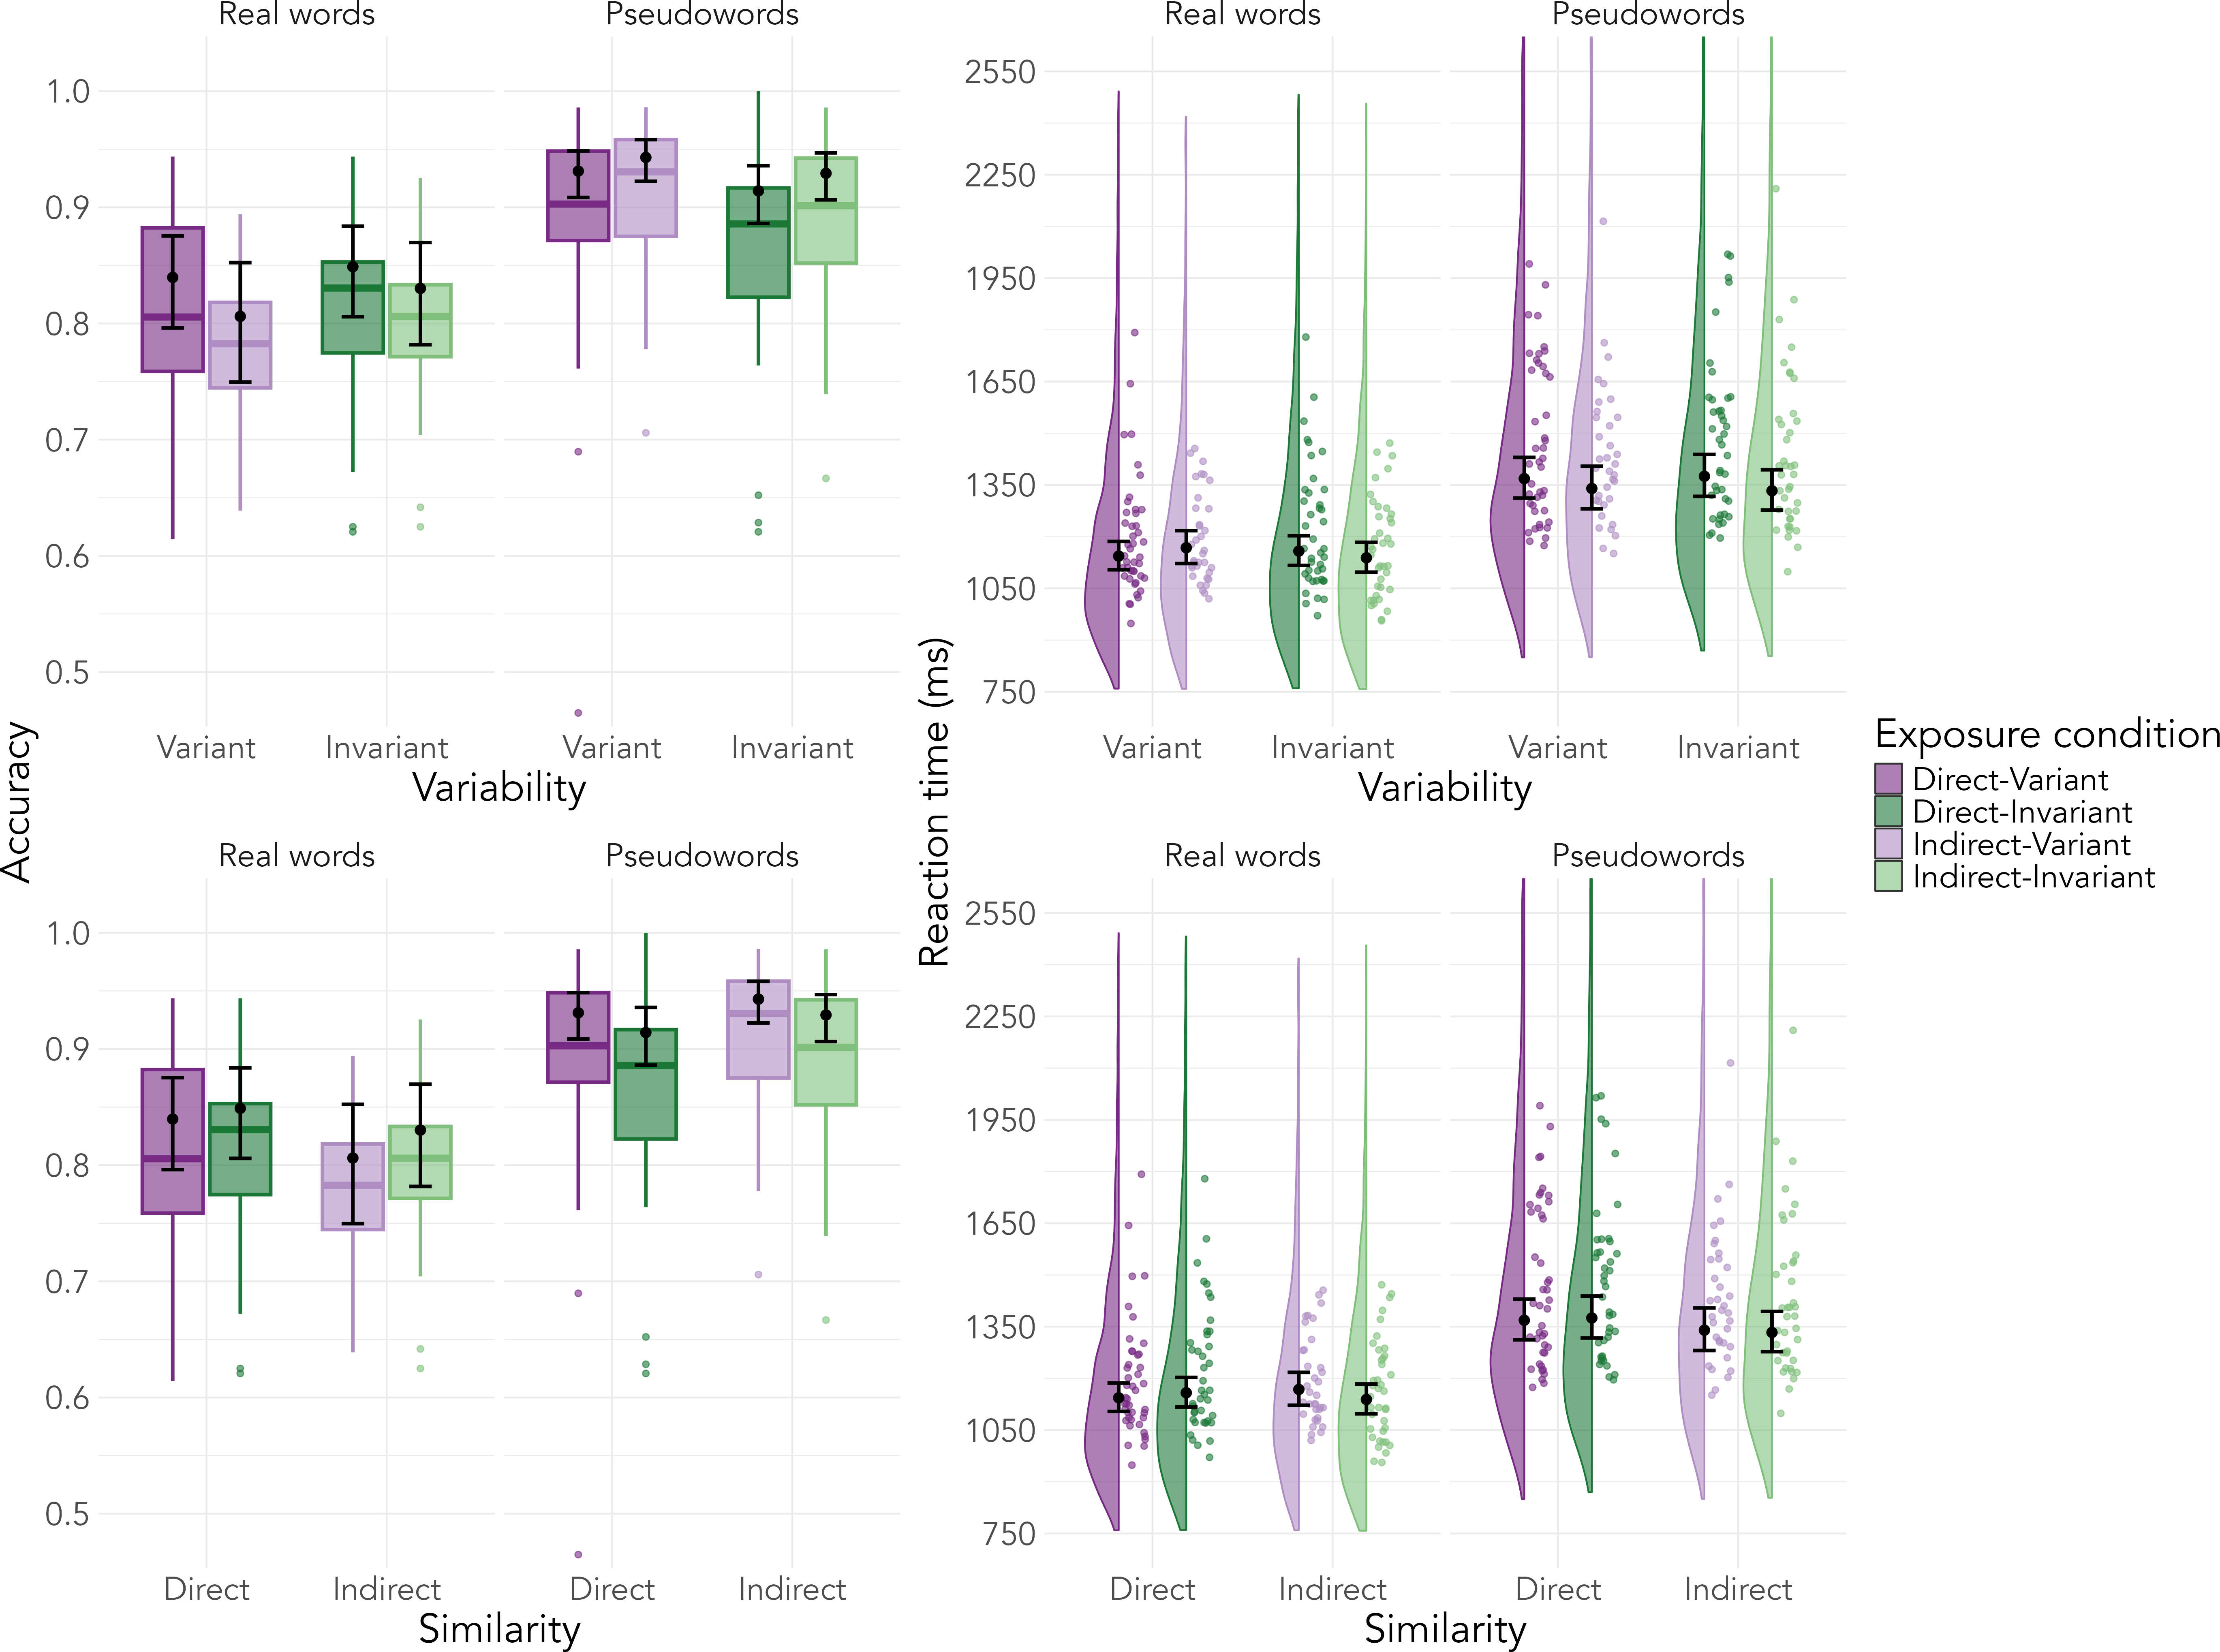
\includegraphics[width=\textwidth]{sections/code/outputs/plot_exp_2} 

}

\caption{Experiment 3 exposure task performance. Left column presents boxplots with mean accuracy by participant. Right column presents half violin plots with reaction times for correct responses and dot plots with mean reaction times for correct responses by participant. Plots are overlaid with estimated marginal means and 95\% confidence intervals.}\label{fig:exp3-exp-fig}
\end{figure}

\hypertarget{test-comparison-to-the-test-only-group-2}{%
\subsubsection{Test: Comparison to the Test-only group}\label{test-comparison-to-the-test-only-group-2}}

For accuracy, we observed a significant interaction between Exposure and Target (\(\chi^2\)(8, \emph{N} = 9) = 49.25, \emph{p} \textless{} .001); however, pairwise comparisons within each level of Target did not reveal any significant differences between the Test-only group and the exposure groups (\emph{ps} \textgreater{} .05).
Comparing the exposure groups to one another, we found that accuracy on Identity targets was significantly higher in the Indirect-Invariant group (\emph{M} = 1.00, 95\% CI {[}1.00, 1.00{]}) than in either the Indirect-Variant group (\emph{M} = 0.99, 95\% CI {[}0.99, 1.00{]}; \emph{z} = 2.89, \emph{p} = .023) or the Direct-Variant group (\emph{M} = 0.99, 95\% CI {[}0.99, 1.00{]}; \emph{z} = 2.62, \emph{p} = .045).
By-participant means and estimated marginal means are shown in the top row of Figure \ref{fig:exp3-test-fig1}.

For RT, we also observed a significant interaction between Exposure and Target (\(\chi^2\)(8, \emph{N} = 9) = 33.56, \emph{p} \textless{} .001).
This interaction was driven by slower RTs on Competitor targets in the Direct-Invariant group (\emph{M} = 690, 95\% CI {[}654, 730{]}) than in the Test-only group (\emph{M} = 631, 95\% CI {[}601, 664{]}; \emph{z} = 2.54, \emph{p} = .044).
Distributions, by-participant means, and estimated marginal means are shown in Figure \ref{fig:exp3-test-fig1}.
To investigate the differences between exposure conditions, we conducted the second set of analyses comparing the effects of Variability and Similarity on RTs.

\begin{figure}

{\centering 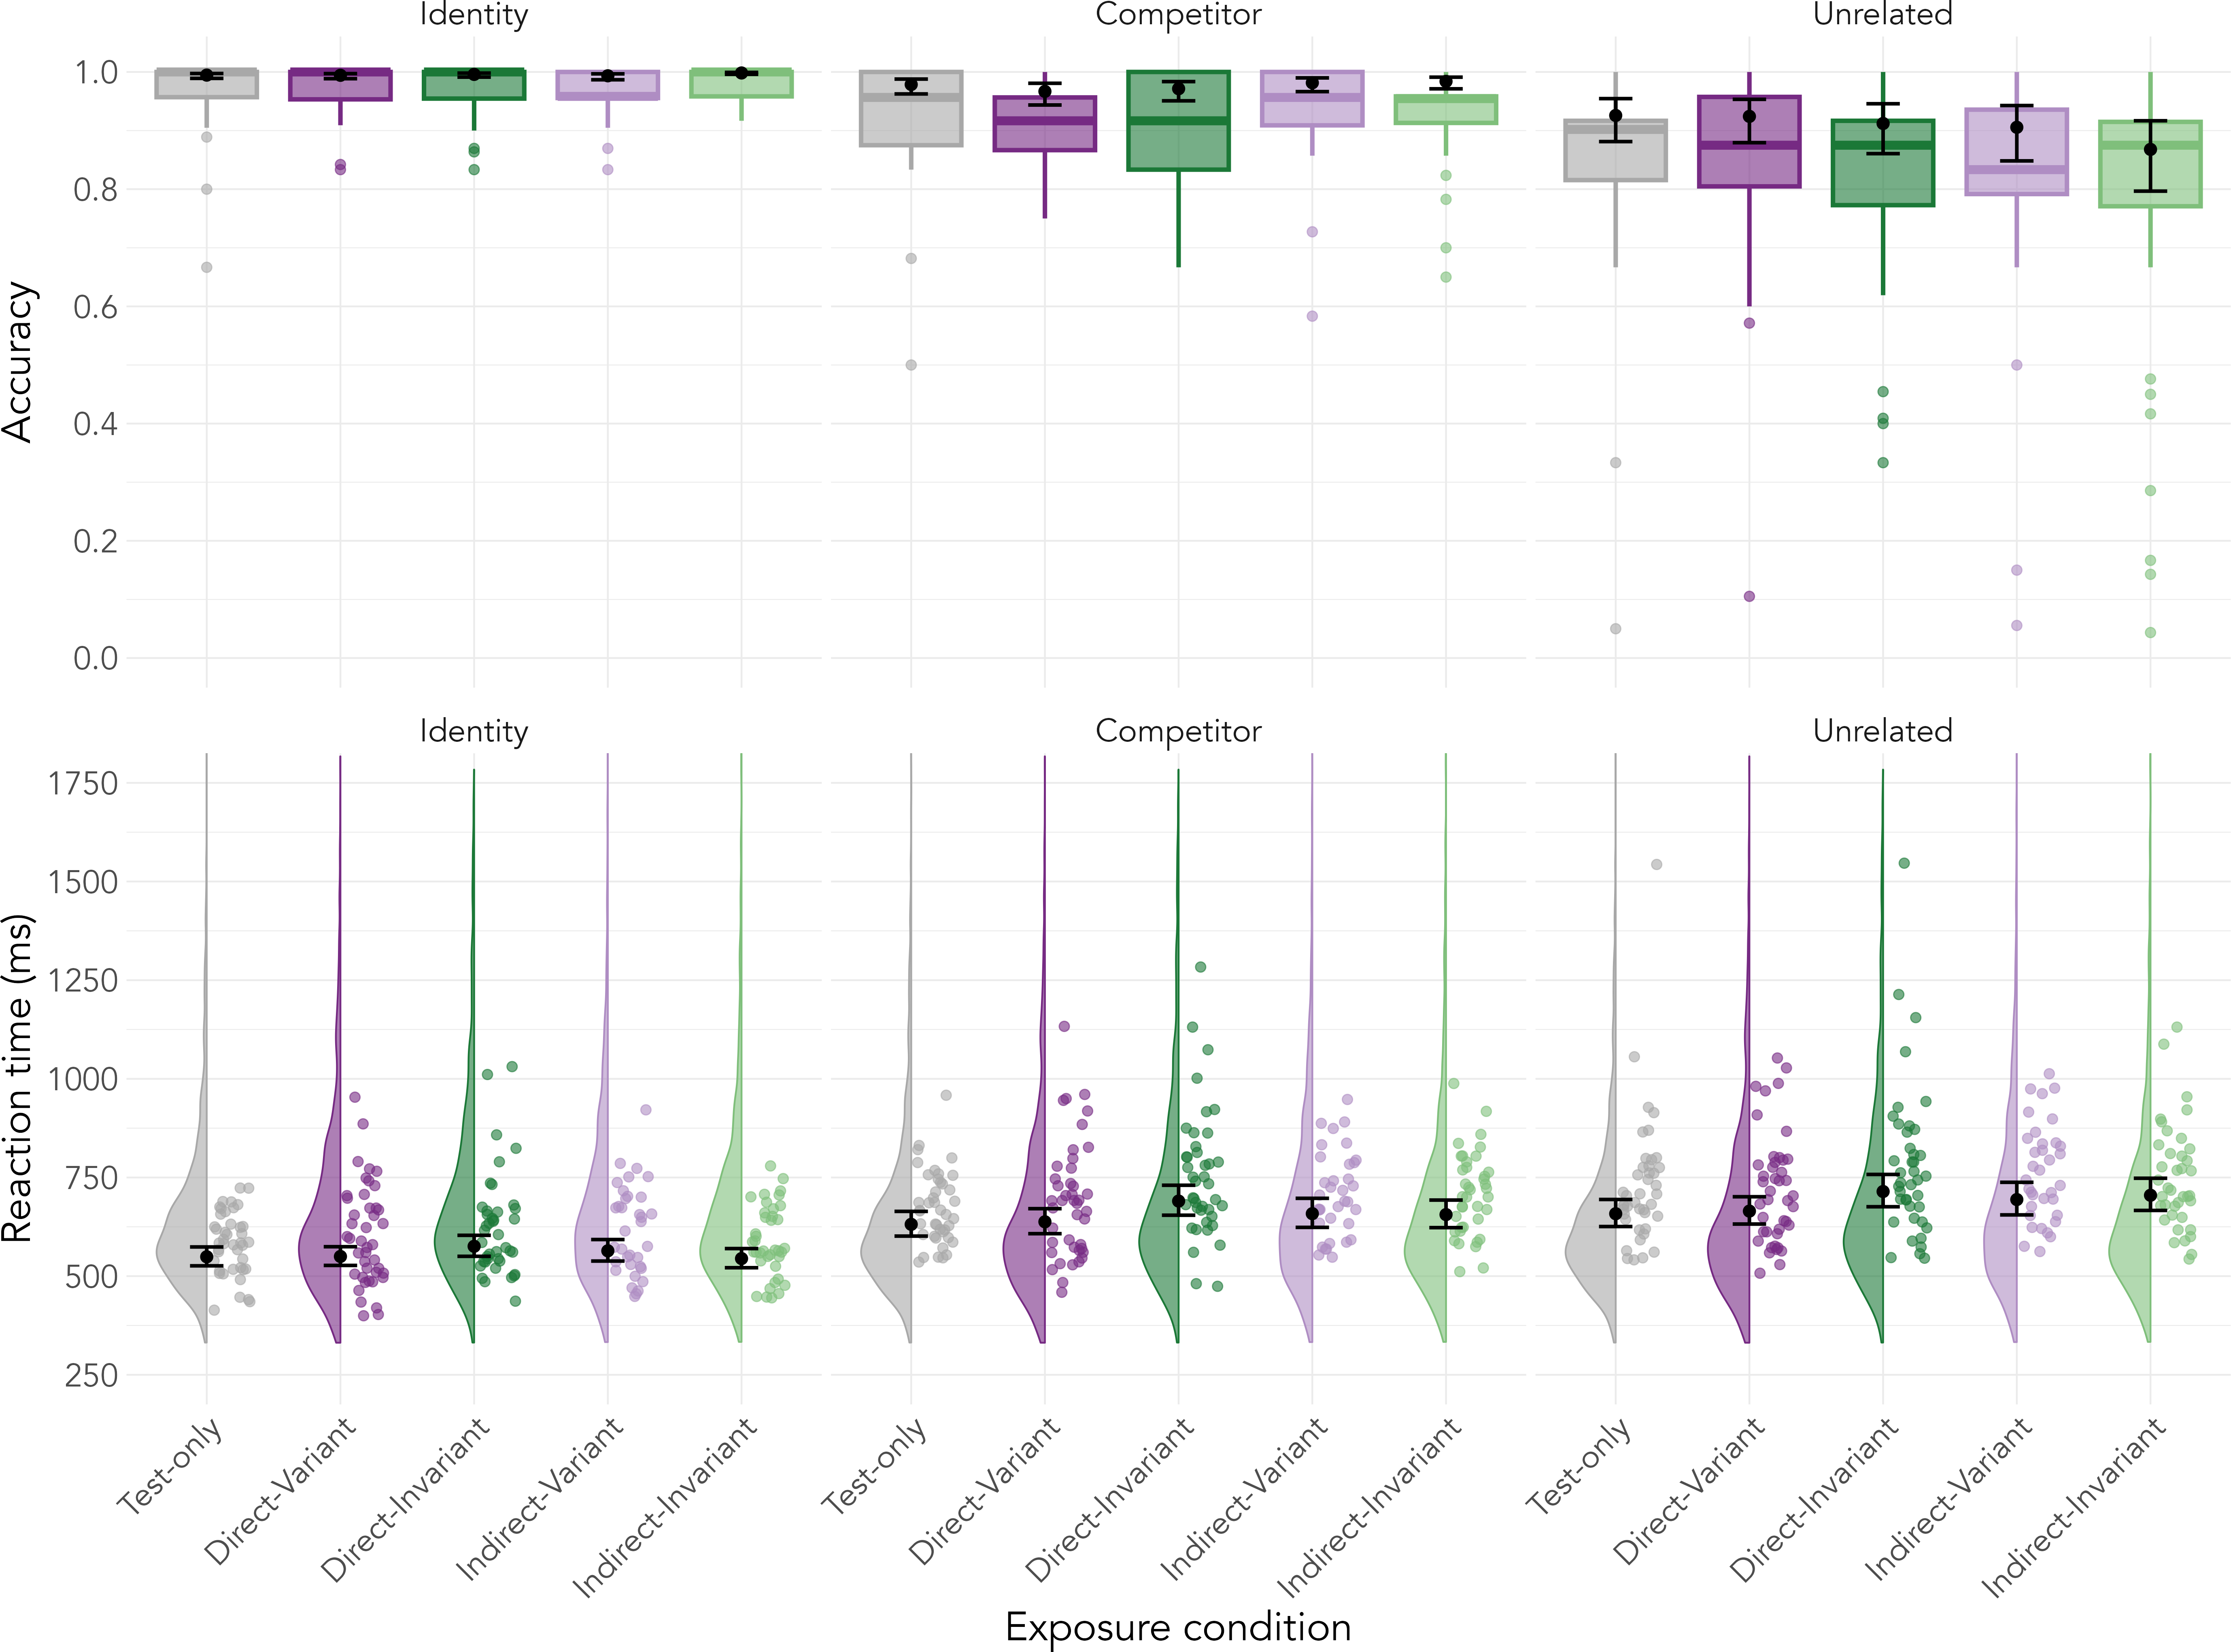
\includegraphics[width=\textwidth]{sections/code/outputs/plot_test_2} 

}

\caption{Experiment 3 test task performance. Top row presents boxplots with mean accuracy by participant. Bottom row presents half violin plots with reaction times for correct responses and dot plots with mean reaction times for correct responses by participant. Plots are overlaid with estimated marginal means and 95\% confidence intervals.}\label{fig:exp3-test-fig1}
\end{figure}

\hypertarget{test-comparison-between-variability-and-similarity}{%
\subsubsection{Test: Comparison between Variability and Similarity}\label{test-comparison-between-variability-and-similarity}}

For RT, we observed significant two-way interactions between Variability and Target (\(\chi^2\)(2, \emph{N} = 3) = 13.87, \emph{p} \textless{} .001) and between Similarity and Target (\(\chi^2\)(2, \emph{N} = 3) = 9.05, \emph{p} = .011).
We followed up on these interactions with separate pairwise comparisons for Variability and Similarity within each level of Target; however, the pairwise comparisons between levels of Variability and between levels of Similarity were not significant (\emph{ps} \textgreater{} .05).
To further probe the source of the interactions in the model, we conducted pairwise comparisons between Direct and Indirect exposure within each combination Target and Variability and between Variant and Invariant exposure within each combination of Target and Similarity.
Within the Competitor level of Target and Direct level of Similarity, Invariant exposure yielded slower RTs (\emph{M} = 691, 95\% CI {[}653, 732{]}) than Variant exposure (\emph{z} = 2.17, \emph{p} = .030).
None of the other pairwise comparisons by Target and Similarity was significant, nor were any of the pairwise comparisons by Target and Variability (\emph{ps} \textgreater{} .05).

\hypertarget{discussion-1}{%
\subsection{Discussion}\label{discussion-1}}

Experiment 3 followed up on the findings of Experiment 2 with a different test task.
Recall that in Experiment 2, we observed significantly higher accuracy on Competitor targets in the Direct-Invariant group than in any of the other exposure groups.
However, the Test-only group performed similarly to the exposure groups, limiting our interpretation of the effects of Variability and Similarity.
We posited that Direct-Invariant training reduced lexical competition between voiced and voiceless stops, thereby increasing correct rejection of Competitor targets as matches for the Spanish-accented auditory primes.
The matching task required participants to explicitly compare the visual target to the auditory prime.
In Experiment 3, we took a more implicit approach.
The priming task probed the extent to which the auditory prime increased or decreased activation of the visual target.
In this way, we could investigate changes in the perception of Spanish-accented stops.

When we compared the four exposure conditions to the Test-only condition, we observed slower RTs for Competitor targets after Direct-Invariant exposure.
We interpret this reduction in speed as a reduction in lexical competition.
For example, consider the auditory prime \emph{park} and the visual target \emph{bark}, which are minimal pairs that differ only in the voicing of their onsets.
The more the onset of \emph{park} is perceived as /b/, the more it will activate the target \emph{bark}.
This increase in activation will facilitate the lexical decision for \emph{bark}, resulting in faster RTs.
Our results suggest that, in the absence of exposure to Spanish-accented speech, Spanish-accented \emph{park} was perceived \textbf{more} like \emph{bark}.
By contrast, with Direct-Invariant exposure, Spanish-accented \emph{park} was perceived \textbf{less} like \emph{bark}.
This reduction in the activation of voiced targets after training suggests that talker-specific exposure to Spanish-accented /p/, /t/, and /k/ improved phonetic categorization of short lag VOTs as voiceless.
Based on this evidence for talker-independent adaptation, we conducted analyses to distinguish the effects of Variability and Similarity.

Within the Direct conditions, Invariant exposure reduced the activation of voiced competitors more than Variant exposure.
This effect was illustrated by significantly slower RTs on Competitor targets for the Direct-Invariant group than for the Direct-Variant group.
As described in the previous paragraph, the Direct-Invariant group was also slower on Competitor targets than the Test-only group.
Together, these results suggest that the Test-only and Direct-Variant groups exhibited similar levels of \emph{park}-\emph{bark} priming, indexing increased activation of /b/ by Spanish-accented /p/.
This finding is striking, considering that the Direct-Variant group had the same amount of exposure to Spanish-accented /p/, /t/, and /k/ from the same talkers as the Direct-Invariant group.
We will interpret this effect of Variability more fully in Section \ref{discuss-study1}.
In short, we will argue that listeners were not able to develop robust talker-independent models during Variant exposure.
Because this level of organization is subject to listeners' use of indexical and social information \citep{kleinschmidt2019}, we will investigate their perceptions of the test talkers in the next section.

\hypertarget{explore-spk}{%
\section{Talker analysis: Characterizing voiceless stop VOT distributions}\label{explore-spk}}

In this section, we analyze the VOT distributions of the talkers.
Table \ref{tab:spk-vot-tab} provides descriptive statistics of the VOT distributions for both voiced and voiceless stops by task, phoneme, and talker.

\begin{table}

\caption{\label{tab:spk-vot-tab}Mean, standard deviation, and range of VOTs by onset by talker.}
\centering
\resizebox{\linewidth}{!}{
\begin{tabular}[t]{l|l|r|r|r|l|r|r|l|r|r|l|r|r|l}
\hline
\multicolumn{3}{c|}{ } & \multicolumn{3}{c|}{Talker 1} & \multicolumn{3}{c|}{Talker 2} & \multicolumn{3}{c|}{Talker 3} & \multicolumn{3}{c}{Talker 4} \\
\cline{4-6} \cline{7-9} \cline{10-12} \cline{13-15}
Phase & Onset & \textit{N} & \textit{M} & \textit{SD} & Range & \textit{M} & \textit{SD} & Range & \textit{M} & \textit{SD} & Range & \textit{M} & \textit{SD} & Range\\
\hline
 & /b/ & 24 & -21 & 51 & -132-48 & 15 & 27 & -87-77 & -44 & 52 & -150-31 & -69 & 53 & -133-103\\
\cline{2-15}
 & /d/ & 24 & 2 & 42 & -100-39 & 21 & 22 & -75-53 & 8 & 29 & -54-33 & -78 & 53 & -177-44\\
\cline{2-15}
 & /g/ & 24 & 2 & 55 & -104-68 & 31 & 25 & -75-51 & -5 & 51 & -148-47 & -64 & 65 & -229-67\\
\cline{2-15}
 & /p/ & 24 & 73 & 26 & 24-122 & 61 & 41 & 11-160 & 82 & 26 & 37-123 & 21 & 17 & 6-69\\
\cline{2-15}
 & /t/ & 24 & 72 & 20 & 36-112 & 65 & 22 & 25-109 & 91 & 28 & 46-157 & 41 & 15 & 18-74\\
\cline{2-15}
\multirow{-6}{*}{\raggedright\arraybackslash Exposure} & /k/ & 24 & 82 & 28 & 33-151 & 88 & 21 & 49-123 & 96 & 23 & 43-133 & 48 & 16 & 25-77\\
\cline{1-15}
 & /p/ & 24 & 71 & 28 & 19-126 & 60 & 35 & 10-118 & 115 & 39 & 15-201 & 26 & 24 & 8-106\\
\cline{2-15}
 & /t/ & 24 & 78 & 21 & 27-109 & 61 & 20 & 28-106 & 102 & 23 & 60-142 & 53 & 27 & 8-99\\
\cline{2-15}
\multirow{-3}{*}{\raggedright\arraybackslash Test} & /k/ & 24 & 94 & 21 & 70-171 & 94 & 20 & 50-133 & 119 & 40 & 65-244 & 65 & 30 & 21-124\\
\hline
\end{tabular}}
\end{table}

\hypertarget{talker-specific-analysis-of-voiceless-stop-vot}{%
\subsection{Talker-specific analysis of voiceless stop VOT}\label{talker-specific-analysis-of-voiceless-stop-vot}}

We first investigate the extent to which each talker's voiceless stop VOTs diverge from L1 US English ``norms,'' which represent our listeners' prior beliefs about these distributions.
We used the VOT dataset compiled by \citet{chodroff2019} to determine the mean VOT for each voiceless stop onset among L1 US English talkers (see Table \ref{tab:spk-vot-mu}).
We then conducted one-sample t-tests to compare each of the talkers' mean VOTs to the norm.
These analyses included both the exposure (multisyllabic) and test (monosyllabic) stimuli (48 items per onset per talker).
Table \ref{tab:spk-vot-mu} provides the difference in means and asterisks indicating the significance level from each analysis (corrected for multiple comparisons with the Hommel method).

\begin{table}

\caption{\label{tab:spk-vot-mu}Mean difference between L1 US English and talker mean VOTs by onset. Asterisks indicate significance levels from two-sample t-tests: *** < .001, ** < .01, * < .05. English means from Chodroff and Wilson (2019).}
\centering
\resizebox{\linewidth}{!}{
\begin{tabular}[t]{l|l|l|l|l|l}
\hline
Phone & L1 US English mean & Talker 1 & Talker 2 & Talker 3 & Talker 4\\
\hline
/p/ & 66 & 6 & -5 & 33*** & -43***\\
\cline{1-6}
/t/ & 78 & -3 & -15*** & 19*** & -31***\\
\cline{1-6}
/k/ & 70 & 18*** & 21*** & 37*** & -14**\\
\hline
\end{tabular}}
\end{table}

\hypertarget{between-talker-analysis-of-voiceless-stop-vot}{%
\subsection{Between-talker analysis of voiceless stop VOT}\label{between-talker-analysis-of-voiceless-stop-vot}}

We next investigate the extent to which each talker's mean VOTs differed from the other talkers'.
This analysis provides a point of comparison to Xie and Myers' (2017) operationalization of exposure-test similarity.
Here, we conducted paired two-sample t-tests on each combination of talkers by onset (48 items per onset per talker).
Table \ref{tab:spk-vot-mat} shows the results of these comparisons, with the value in each cell being the column talker's mean minus the row talker's mean.

\begin{table}

\caption{\label{tab:spk-vot-mat}Mean difference in VOT between talkers by onset. Asterisks indicate significance levels from paired two-sample t-tests corrected with Hommel method: *** < .001, ** < .01, * < .05.}
\centering
\resizebox{\linewidth}{!}{
\begin{tabular}[t]{l|l|l|l|l|l}
\hline
Comparison & Exposure onset & Talker 1 & Talker 2 & Talker 3 & Talker 4\\
\hline
 & /p/ &  & -11 & 27** & -49***\\
\cline{2-6}
 & /t/ &  & -12* & 22*** & -28***\\
\cline{2-6}
\multirow{-3}{*}{\raggedright\arraybackslash Talker 1} & /k/ &  & 3 & 19** & -32***\\
\cline{1-6}
 & /p/ & 11 &  & 38*** & -37***\\
\cline{2-6}
 & /t/ & 12* &  & 34*** & -16**\\
\cline{2-6}
\multirow{-3}{*}{\raggedright\arraybackslash Talker 2} & /k/ & -3 &  & 16* & -35***\\
\cline{1-6}
 & /p/ & -27** & -38*** &  & -75***\\
\cline{2-6}
 & /t/ & -22*** & -34*** &  & -50***\\
\cline{2-6}
\multirow{-3}{*}{\raggedright\arraybackslash Talker 3} & /k/ & -19** & -16* &  & -51***\\
\cline{1-6}
 & /p/ & 49*** & 37*** & 75*** & \\
\cline{2-6}
 & /t/ & 28*** & 16** & 50*** & \\
\cline{2-6}
\multirow{-3}{*}{\raggedright\arraybackslash Talker 4} & /k/ & 32*** & 35*** & 51*** & \\
\hline
\end{tabular}}
\end{table}

\hypertarget{discussion-2}{%
\subsection{Discussion}\label{discussion-2}}

The two analyses conducted in this section show that our talkers differed from both L1 US English norms and one another in their VOT distributions.
Talker 4 produced the most Spanish-like VOT distributions across places of articulation, with significantly shorter means in all comparisons.
Talker 3 also differed from the L1 US English norms and the three other talkers, but in the opposite direction: her mean VOTs were significantly longer in all comparisons.
Talkers 1 and 2 were the most similar to one another, with statistically equivalent mean VOTs for /p/ and /k/.
Talker 1 was the most similar to the L1 US English norms, though both she and Talker 2 had significantly longer /k/ VOTs.
Overall, each talker exhibited a unique pattern of VOT-stop distributions.
We discuss the implications of these results for our Similarity and Variability manipulations in the next section.

\hypertarget{discuss-study1}{%
\section{General discussion}\label{discuss-study1}}

The current study investigated generalization of exposure to L2-accented speech.
We compared two hypotheses with different explanations for how exposure supports talker-independent adaptation.
The exposure-to-variability hypothesis argues that increasing covariation between acoustic-phonetic cues during exposure increases performance on a new talker \citep{baese2013, bradlow2008}.
The similarity-based hypothesis argues that increasing cue-category overlap between the exposure and test talkers increases performance on the test talker \citep{xie2017similarity}.
We expressed these hypotheses in terms of the ideal adapter framework to investigate their explanatory power within the same theoretical model \citep{kleinschmidt2015}.
Under this theory, listeners develop mental models of the mappings between acoustic cues (like VOT) and phonetic categories (like /p/, /t/, and /k/) according to informative and useful social (here, L2 accent) and indexical (talker) groupings \citep{kleinschmidt2019}.
To restate the two competing hypotheses using this framework, exposure to variability enhances the formation of talker-independent generative models, while exposure-test similarity facilitates the selection of talker-specific generative models.
Using a novel experimental approach that improved the scope and precision of how variability and similarity are operationalized, we conducted a series of three experiments.
The combined results provide strongest support for the similarity-based hypothesis.

The key findings come from Experiment 3.
After exposure to three Spanish-accented English talkers, we measured performance on a novel Spanish-accented English talker with a primed cross-modal lexical decision task.
The critical items in this task were monosyllabic auditory primes with voiceless stop onsets: for example, \emph{park}, \emph{tune}, and \emph{coal}.
Importantly, these items had onset competitors with the same place and manner of articulation: \emph{bark}, \emph{dune}, and \emph{goal}, respectively.
Participants made lexical decisions on the visual targets that followed these critical primes.
Performance on the different target types indexed different aspects of perceptual adaptation.
Specifically, priming of Identity targets indexed lexical activation of the intended word, while priming of Competitor targets indexed lexical activation of perceptually similar words.
For example, consider the auditory prime \emph{park}.
The Identity target for this prime is \emph{park}, while the Competitor target for this prime is \emph{bark}.
If perceptual adaptation to Spanish-accented speech increased activation of the lexical item ``park'' upon hearing \emph{park}, then responses to the visual target \emph{park} would also increase.
If perceptual adaptation to Spanish-accented speech decreased activation of the lexical item ``bark'' upon hearing \emph{park}, then responses to the visual target \emph{bark} would also decrease.
Ideally, exposure would both increase activation of the intended word and decrease activation of competing words.
However, we found that Direct-Invariant exposure decreased lexical competition without increasing lexical activation.
Specifically, the Direct-Invariant group displayed significantly slower RTs on Competitor targets than both the Test-only group and Direct-Variant group, but did \emph{not} display significantly faster RTs on Identity targets.
Thus, the decrease in lexical competition we observed was not related to an increase in lexical activation for the intended word.
In the next section, we compare our findings to the predictions of the exposure-to-variability and similarity-based hypotheses.

\hypertarget{exposure-to-variability-versus-similar-exposure}{%
\subsubsection{Exposure to variability versus similar exposure}\label{exposure-to-variability-versus-similar-exposure}}

The exposure-to-variability hypothesis is based on the findings of \citet{baese2013}.
In that study, exposure to multiple talkers, each with a different L2 accent, generalized to a novel talker with an unfamiliar L2 accent.
Exposure to multiple talkers with the same L2 accent did not generalize to an unfamiliar L2 accent \citep{bradlow2008}.
However, both types of exposure generalized to a novel talker with a familiar L2 accent.
The multi-accent condition included one Mandarin-accented talker out of five talkers with different L1s, while the single-accent condition included five Mandarin-accented talkers.
In both cases, performance on a novel Mandarin-accented talker was higher than in the control condition.
Together, these results suggest that listeners benefit from exposure to systematic covariation across L2 accents.
In other words, the ways in which L2 varieties differ from L1 varieties at a high level generalizes across L2 talkers.
This hypothesis is also supported by recent work on cross-accent generalization \citep{bradlow2023}, as well as by the large body of work on high-variability phonetic training for L2 acquisition \citep[for a review, see][]{zhang2021hvpt}.

By contrast, the similarity-based hypothesis comes from \citet{xie2017similarity}.
In this study, two groups of participants trained on multiple Mandarin-accented talkers.
The experimental group was exposed to disambiguating lexical contexts for word-final /d/ (e.g., \emph{overload}), while the other was not.
During test on a novel Mandarin-accented talker, lexical activation for /d/-final primes was higher in the experimental group.
Among the Mandarin-accented talkers in the training set, one talker's productions of /d/ were similar to those of the test talker on multiple acoustic measures.
There was also one talker out of the five whose productions of /d/ differed from the test talker's on these metrics.
After single-talker exposure to the similar talker, lexical activation for /t/-final competitors was lower in the experimental group.
By contrast, single-talker exposure to the dissimilar talker did not reduce lexical competition.
Overall, single-talker exposure to the similar talker and multi-talker exposure including the similar talker both facilitated generalization to a novel talker.
This suggests that the specific way in which an L2-accented talker produces an L2 variety determines the level of generalization to other talkers.
This hypothesis is supported by work on lexically-guided perceptual retuning showing different patterns of generalization for different phonetic contrasts \citep{kraljic2006, kraljic2007, reinisch2014}.

Having revisited the two competing hypotheses that motivated our work, we return to the specific predictions and results.
The exposure-to-variability hypothesis predicted a main effect of Variability, with better test performance after Variant versus Invariant exposure.
Participants in both conditions were also expected to outperform the Test-only group.
This hypothesis does not make predictions regarding activation of intended words (Identity targets) versus activation of competing words (Competitor targets).
However, given that the hypothesis is based on research where transcription accuracy is the measure of generalization, Variant exposure was likely to emerge on Identity target performance.
The similarity-based hypothesis predicted a main effect of Similarity, with better test performance after Direct versus Indirect (or Control) exposure.
Participants in the Direct condition were also expected to outperform the Test-only group.
Specifically, Direct exposure was expected to both increase activation for intended words and decrease activation for competitors.

Our results provided evidence for the similarity-based hypothesis and against the exposure-to-variability hypothesis.
In both Experiments 2 and 3, Direct-Invariant exposure decreased activation for competitors.
Specifically, we observed an increase in RTs for Competitor targets in the Direct-Invariant group relative to both the Test-only group and the Direct-Variant group in Experiment 3.
In Experiment 2, we observed an increase in accuracy on Competitor targets in the Direct-Invariant group relative to all three exposure groups.
The performance benefits from Direct exposure align best with the predictions of the similarity-based hypothesis.
In addition, the performance benefits from Invariant exposure contrast the predictions of the exposure-to-variability hypothesis.
To better understand these findings, we return to how we operationalized Similarity and Variability relative to previous research.

\hypertarget{discuss-sim}{%
\subsubsection{Implementing similarity}\label{discuss-sim}}

Regarding similarity, we exposed participants to different sets of Spanish-accented stops through an auditory lexical decision task.
In Direct conditions, participants gained experience with /p/, /t/, and /k/ onsets in the context of real words like \emph{peanut}, \emph{terminal}, and \emph{kingdom}, respectively.
Exposure to Spanish-accented voiceless stops trained listeners to shift the VOT distributions for these sound categories from long lag (English-like) toward short lag (Spanish-like).
In Indirect conditions, participants gained experience with /b/, /d/, and /g/ in the context of real words like \emph{beehive}, \emph{desert}, and \emph{gallop}, respectively.
Exposure to Spanish-accented voiced stops trained listeners to shift the VOT distributions for these sound categories from short lag (English-like) toward lead (Spanish-like).
Shifting the VOT distribution for voiced stops leftward on the cue continuum had the potential to trigger a more general leftward shift that would move the VOT distributions for voiceless stops from long lag to short lag.
This approach to investigating similarity involved exposure to different sound categories.

By contrast, the approach of \citet{xie2017similarity} involved exposure to different cue distributions over the same sound category.
That study compared the means of three different cues to voicing in word-final position to determine which talker had the most (dis)similar cue-category distributions to the test talker; separate groups of participants were then exposed to either the similar talker or the dissimilar talker.
As a result, their design featured different talkers across exposure conditions.
Our design featured the same talkers across exposure conditions, allowing us to control the amount of talker-specific acoustic-phonetic variability between levels of Similarity.
In turn, this allowed us to manipulate the constructs of Similarity and Variability independently.
We did not, however, control the exact VOT-stop distributions that listeners heard during exposure.
We ultimately found in Section \ref{explore-spk} that Talker 4 was the only one of the four with consistently Spanish-accented voiceless stops.

The fact that our talkers produced less ambiguous voiceless stops than expected may have weakened the adaptation effects we observed; however, it did not disrupt the Similarity manipulation itself.
The VOT distributions for the /p/, /t/, and /k/ onsets in the Direct exposure conditions were distinct from those for the /b/, /d/, and /g/ onsets in the Indirect exposure conditions.
Critically, they were also similar to those for the test items.
As a result, Direct exposure was both useful and informative for adapting to the test talker in a way that Indirect exposure was not.
We also note that it is relatively uncommon in the L2-accented speech recognition literature to report acoustic-phonetic measures at all \citetext{\citealp[cf.][]{xie2021}; \citealp[@][]{alexander2019}}, even though they presumably comprise what we perceive as an accent itself.
In the present study, these measures help us understand the structure of our listeners' generative models for Spanish-accented speech, as we describe in the next section.

\hypertarget{discuss-var}{%
\subsubsection{Implementing variability}\label{discuss-var}}

Regarding variability, we exposed participants to different combinations of talker and onset.
In Variant conditions, participants gained experience with the VOT distributions for each onset across talkers.
Since there were 24 real word stimuli per onset, this means that each of the three talkers produced eight experimental items with each onset.
In Invariant conditions, participants gained experience with the VOT distributions for each onset within talkers.
This means that each talker produced 24 experimental items with a single onset.
The variability manipulation was also extended to the filler items, with two filler onsets assigned to each talker.
Overall, listeners heard 72 real words from each talker during exposure.

By contrast, in \citet{bradlow2008} and \citet{baese2013}, participants in the multi-talker exposure groups heard 16 sentences with 50 total key words per talker.
While each set of sentences was different for each exposure talker, participants completed five repetitions per talker, increasing the total amount of exposure to each talker to 250 key words.
This is nearly three times the amount of word-level exposure to each talker compared to our study.
Previous research has shown that listeners need significantly more exposure to adapt to multiple talkers compared to a single talker \citep{luthra2021}.
Even in a talker-specific paradigm, test performance increases with increasing evidence for adaptation \citep{cummings2023}.
Thus, the relatively limited amount of exposure our participants had to variability may have limited the strength of its benefits.
However, the amount of exposure did not differ between our levels of Variability.
Moreover, we observed a clear benefit for Invariant versus Variant exposure.
We interpret this finding in terms of the specificity of generative models.

According to \citet{kleinschmidt2019}, generative models can be constructed according to an individual person (talker-specific) or a higher-level social category (talker-independent).
The level of organization is determined by two factors.
First, the model needs to be a good representation of the actual distribution.
That is, the cue-category mappings that the listener has heard need to be captured by the mental representation (i.e., informative).
Second, the model needs to be a good predictor of future exemplars.
In other words, the mental representation needs to help listeners categorize a given instance of a cue as a particular category (i.e., useful).
In our experiment, we gave listeners different samples of each talker's VOT distributions.
We can illustrate this idea with hypothetical Talker A and her VOT-/p/ mapping.
Variant exposure give listeners a small sample of Talker A's VOT-/p/ mapping relative to Invariant exposure, where all VOT-/p/ mappings are from Talker A.
Direct exposure allows listeners to sample Talker A's VOT distribution for /p/, while Indirect exposure only allows listeners to sample her VOT distribution for the voiced counterpart /b/.
These different samples influenced how listeners constructed their representations.

As explained in Section \ref{discuss-1b}, talker-specific generative models were the only possible representations of Invariant exposure.
This is because Invariant exposure only provided one talker's cue distributions for a given category.
With Variant exposure, both talker-specific and talker-independent models were possible; however, talker-independent models were optimal.
This is because there were only 24 exemplars of each phonetic category divided among three talkers.
Thus, talker-specific models would have been developed from a relatively sparse sample of eight exemplars.
If we assume that the talkers had similar VOT-stop distributions, the talker-specific generative models developed during Invariant exposure should have been as useful as the talker-independent generative models developed during Variant exposure.
However, the reduction in lexical competition we observed following Direct-Invariant exposure compared to Direct-Variant exposure suggests that this was not the case.

There are two possible explanations.
First, the talker-independent generative models that listeners developed from Variant exposure were not as useful as the talker-specific generative models that listeners developed from Invariant exposure.
Second, listeners developed talker-specific generative models regardless of variability, which led to sub-optimal representations of Variant exposure.
Both of these accounts would be consistent with exposure to different VOT distributions for each talker.
The post-hoc talker analysis in Section \ref{explore-spk} showed that this was indeed the case.
We found that mean VOTs differed between all four talkers at almost every place of articulation.
A third explanation would be that exposure to such distinct Spanish-accented talkers would result in a general relaxation of categorization criteria (rather than shifts in categorization boundaries); however, if this were the case, we would not have observed any differences in performance as a function of exposure group.
Rather, we observed a unique benefit of Direct-Invariant exposure broadly consistent with the similarity-based hypothesis.
In terms of the ideal adapter framework, these findings suggest that developing talker-specific generative models for multiple talkers may be the best approach when between-talker variation is high.

\hypertarget{conclusion}{%
\subsubsection{Conclusion}\label{conclusion}}

Overall, our results show that talker-independent adaptation to L2-accented speech is facilitated by exposure-test similarity.
We also found evidence that generalization is enhanced when between-talker variability is limited, at least for the rapid adaptation effects we investigated here.
This study is the first to compare variability and similarity while maintaining the same talkers across conditions.
This level of control is key to understanding how exposure to between-talker variability interacts with exposure to specific acoustic-phonetic properties.
We suggest that the contradictory findings in the literature are at least partially a result of comparing different talkers, who have idiosyncratic patterns of within-talker covariation \citep{clayards2017, whalen2018, xie2020}.
Listeners are highly sensitive to variation in speech, particularly during perception.
In future work, we hope to better understand how this sensitivity is deployed during talker- and category-independent adaptation to L2-accented speech.

\bibliography{dissertation.bib}


\end{document}
